% !TeX spellcheck = pl_PL-Polish
%\documentclass[xcolor=pdftex,dvipsnames,table]{beamer}
%\documentclass[dvipsnames]{beamer}
\documentclass[11pt, xcolor={dvipsnames,svgnames},aspectratio=169]{beamer}
%\hypersetup{colorlinks}1
\usepackage{etex} % tikz needs it
\usepackage[utf8]{inputenc}
\usepackage{polski}
\usepackage[OT4]{fontenc} % doesn't change - default, and best?
%\usepackage[T1]{fontenc} % thinner, a bit more machine like
%\usepackage{times} % serif
\usepackage{amsfonts}
\usepackage{amsmath}
\usepackage{amsthm}
\usepackage{amsbsy}
\usepackage{amscd}
\usepackage{bbm}
\usepackage[mathscr]{eucal} 
%\usepackage{subfigure}
\usepackage{pifont}
\usepackage{color}
\usepackage{booktabs}
\usepackage{colortbl}
\usepackage{marvosym}
\usepackage{wasysym}
\usepackage[normalem]{ulem}
\usepackage{multicol}
\usepackage[makeroom]{cancel}
\usepackage{soul}
\definecolor{orange}{rgb}{0.75,0.33,0}
\newcommand{\myemph}[1]{\textcolor{orange}{#1}}

\usepackage{tikz}
\usetikzlibrary{matrix,positioning}

\usepackage{isomath}
\usepackage{soul}
%\usepackage{ctable}

\renewcommand\mathfamilydefault{\rmdefault}

\newcommand{\attr}[1]{\tiny\begin{flushright}(source: #1)\end{flushright}\normalsize
}
\newcommand{\attrl}[1]{\tiny\begin{flushleft}(source: #1)\end{flushleft}\normalsize
}
%\newcommand{\source}[1]{\tiny\begin{flushright}(źródło ilustacji: \texttt{#1})\end{flushright}\normalsize}

 
\usetheme{iitisask}
\title[]{Statystyczne metody uczenia maszynowego --\\ redukcja wymiarowości i klasyfikacja}
\author{Przemysław Głomb}
\date{redaktor pomocniczy: Bartłomiej Gardas}

\theoremstyle{plain}
\newcommand{\scaly}{0.7}

\theoremstyle{plain}
	
 
\begin{document}


\frame{\maketitle}


\section{Metody liniowe}

\subsection{Analiza składowych głównych}

\begin{frame}
	\frametitle{Macierz kowariancji, odległość Mahalanobisa, RX, \dots}
	\begin{center}
		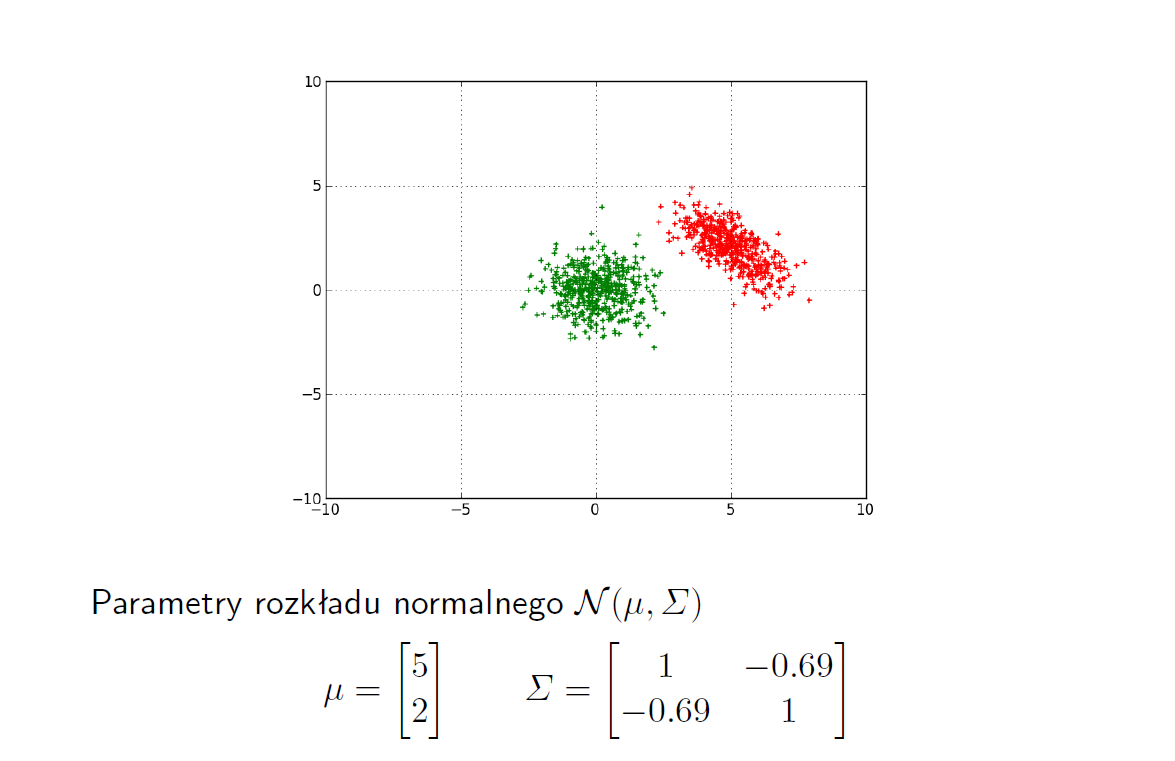
\includegraphics[width=0.3\textwidth]{images/ncov.png}
		%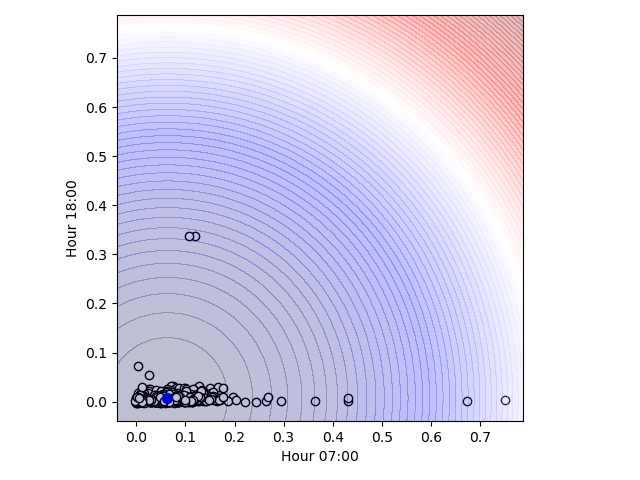
\includegraphics[width=0.24\textwidth]{images/eye.png}
		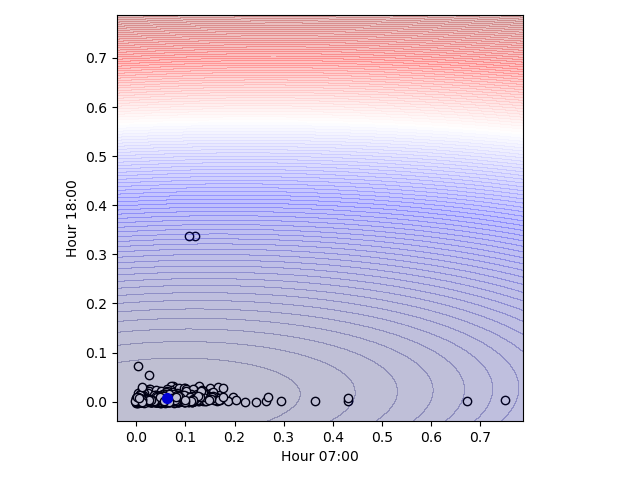
\includegraphics[width=0.3\textwidth]{images/C.png}
		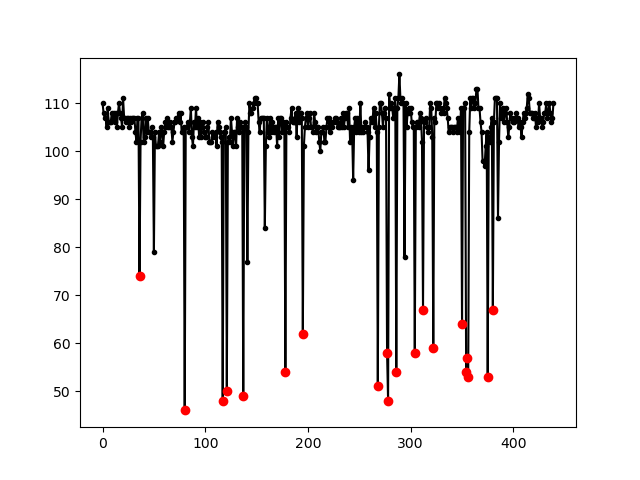
\includegraphics[width=0.3\textwidth]{images/rxha.png}
	\end{center}
\end{frame}

\begin{frame}
	\frametitle{Zbiory danych są wielowymiarowe}
	\begin{description}
		\item[1 cecha] przykład z wykładu o perceptronie - dojrzałość owocu\pause
		\item[2 cechy] właściwości przeciwrakowe peptydów (sekwencja dna, aktywność)\only<2>{\footnote{Grisoni, F., Neuhaus, C.S., Hishinuma, M., Gabernet, G., Hiss, J.A., Kotera, M. and Schneider, G., 2019. De novo design of anticancer peptides by ensemble artificial neural networks. Journal of Molecular Modeling, 25(5), 112}}\pause
		\item[5 cech] predykcja awarii silników wentylatora na podstawie danych z akcelerometrów\only<3>{\footnote{Scalabrini Sampaio, G., Vallim Filho, A. R. d. A., Santos da Silva, L., \& Augusto da Silva, L. (2019). Prediction of Motor Failure Time Using An Artificial Neural Network. Sensors, 19(19), 4342}}\pause
		\item[10 cech] predykcja właściwości rozbłysków słonecznych\only<4>{\footnote{\url{https://archive.ics.uci.edu/dataset/89/solar+flare}}}\pause
		\item[24 cechy] klasyfikacja choroby nerek na podstawie parametrów biochemicznych\only<5>{\footnote{\url{https://archive.ics.uci.edu/dataset/336/chronic+kidney+disease}}}\pause
		\item[127 cech] predykcja parametrów przestępstw i wykroczeń na podstawie danych socjoekonomicznych\only<6>{\footnote{Redmond, Michael and Alok Baveja. “A data-driven software tool for enabling cooperative information sharing among police departments.” Eur. J. Oper. Res. 141 (2002): 660-678. } }\pause
		\item[1203 cechy] Toksyczność cząsteczek mających wpływ na zegar biologiczny\only<7>{\footnote{Gul, S., Rahim, F., Isin, S. et al. Structure-based design and classifications of small molecules regulating the circadian rhythm period. Sci Rep 11, 18510 (2021)} }\pause
		\item[65 tys. cech] obrazek $256\times 256$\pause
		\item[150 tys. cech] Zespół czujników gazowych wystawiony na działanie turbulentnych mieszanek gazowych\only<9>{\footnote{\url{https://archive.ics.uci.edu/dataset/309/gas+sensor+array+exposed+to+turbulent+gas+mixtures}}}\pause
		\item[3+ mln cech] reputacja adresów URL\only<10>{\footnote{\url{https://archive.ics.uci.edu/dataset/187/url+reputation} } }\pause
	\end{description}
\end{frame}

\begin{frame}
	\frametitle{1203 cechy? 150 tys. cech? Miliony cech?}
	\begin{itemize}
		\item Trudność inspekcji (tysiące $\rightarrow$ miliony przykładów)\pause
		\item Złożoność -- wymagana ,,pojemność'' modelu (zdolność do reprezentacji)\pause 
			\begin{itemize}
				\item Trudność doboru modelu, architektury
				\item Czas trwania przygotowania modelu
				\item Zasoby pamięciowe i obliczeniowe na przygotowanie i testowanie modelu\pause
			\end{itemize}
		\item Właściwości przestrzeni wielowymiarowych\pause
			\begin{itemize}
				\item Przekleństwo wymiarowości (\textbf{curse of dimensionality})
			\end{itemize}
	\end{itemize}
\end{frame}

\begin{frame}
	\frametitle{Przekleństwo wymiarowości}
	\begin{itemize}
		\item Rzadkość danych w przestrzeniach wielowymiarowych\pause\only<2>{\begin{center}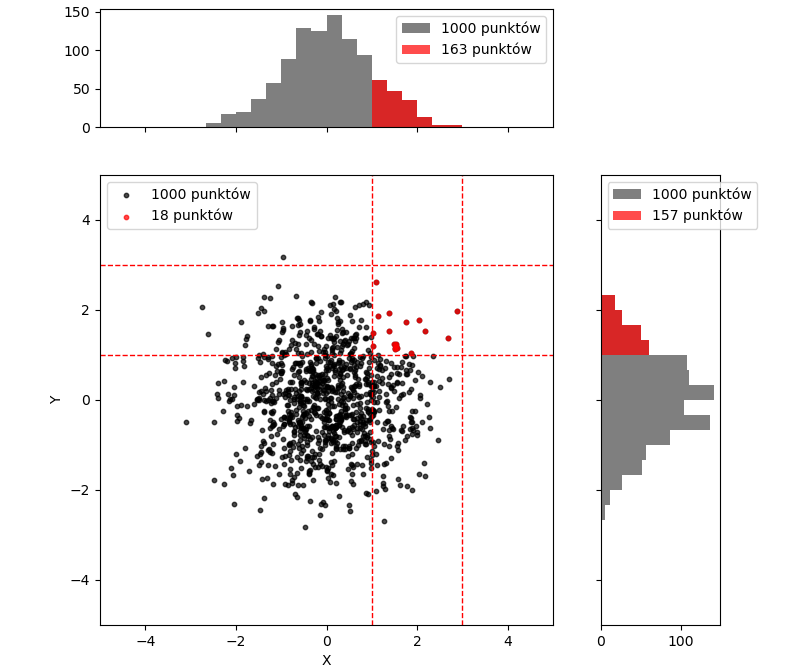
\includegraphics[width=0.45\textwidth]{images/cod.png}\end{center}}\pause
		\item ,,Ucentrowienie'' (hubness), np. przy szukaniu podobnych przykładów
		\item Wymagania liczby punktów danych $n > d, n \geq 10d, n \gg d$
		\item Wymagania obliczeniowe i pamięciowe
		\item Trudność oszacowania parametrów statystycznych (korelacje, outliery)
	\end{itemize}
\end{frame}

\begin{frame}
	\frametitle{Korelacje między cechami}
	Intuicja:\\
	\begin{itemize}
		\item Dane z urządzeń IoT mierzących temperaturę, wilgotność itp. w mieście\pause
		\item Film z kamery monitoringu parkingu\pause 
		\item Dane mieszkań: cena, rozmiar, liczba pokojów, liczba łazienek, miejsce dodatkowe (piwnica/garaż)\pause
		\item Zużycie wody w okresie godzinowym w ciągu tygodnia\pause
	\end{itemize}
	\vskip 0.5 cm
	Reprezentacja korelacji:
	\begin{itemize}
		\item Nazwane cechy (np. cena mieszkania i rozmiar w m$^2$)\pause
		\item Nie nazwane cechy (np. piksele obrazka)
	\end{itemize}
\end{frame}

\begin{frame}
	\frametitle{Dekorelacja}
	Intuicja:
	\only<1>{	\begin{center}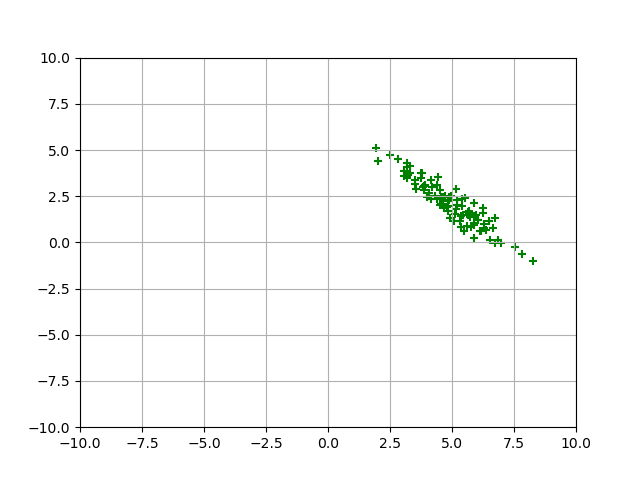
\includegraphics[width=0.5\textwidth]{images/pcatoy1.png}	\end{center}}\pause
	\only<2>{	\begin{center}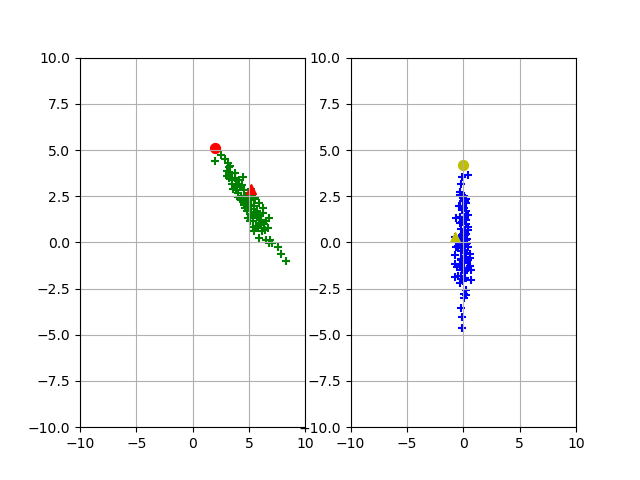
\includegraphics[width=0.5\textwidth]{images/pcatoy2.png}	\end{center}}	
\end{frame}

\begin{frame}
	\frametitle{Analiza składowych głównych -- wyznaczanie}
	\begin{enumerate}
		\item Zbiór przykładów $\mathcal{X}$\\$\mathcal{X}=\left\{\mathbf{x}_1, \mathbf{x}_2, \dots, \mathbf{x}_m\right\}$\\ $\mathbf{x}_i=(x_{i1}, x_{i2}, \dots, x_{in})$, $x_{ij}\in\mathbb{R}$\pause
		\item Zbiór po odjęciu średniej\\
		$\mathbf{x}_i'=\mathbf{x}_i - \frac{1}{m}\sum_{i=1}^m \mathbf{x}_i=\mathbf{x}_i - \bar{\mathbf{x}}$\\\pause
		zapisujemy w postaci macierzy\\$X=\begin{bmatrix}
			x_{11}' & x_{12}' & \dots\\
			x_{21}' & x_{22}' & \dots\\	
			\dots & \dots & x_{mn}'
		\end{bmatrix}$\pause
		\item Wyznaczamy macierz kowariancji\\
		$S= \frac{1}{m-1}X X^\top$\\\pause
		i jej wektory własne (posortowane po wartościach własnych) układamy w macierz $A$\pause
		\item Dla dowolnego (w ramach rodziny danych) wektora $x$ uzyskujemy składowe z równania\\
		$\mathbf{c} = A(\mathbf{x} - \bar{\mathbf{x}})$
	\end{enumerate}
\end{frame}

\begin{frame}\frametitle{Analiza składowych głównych -- przykład/idea działania}
\begin{center}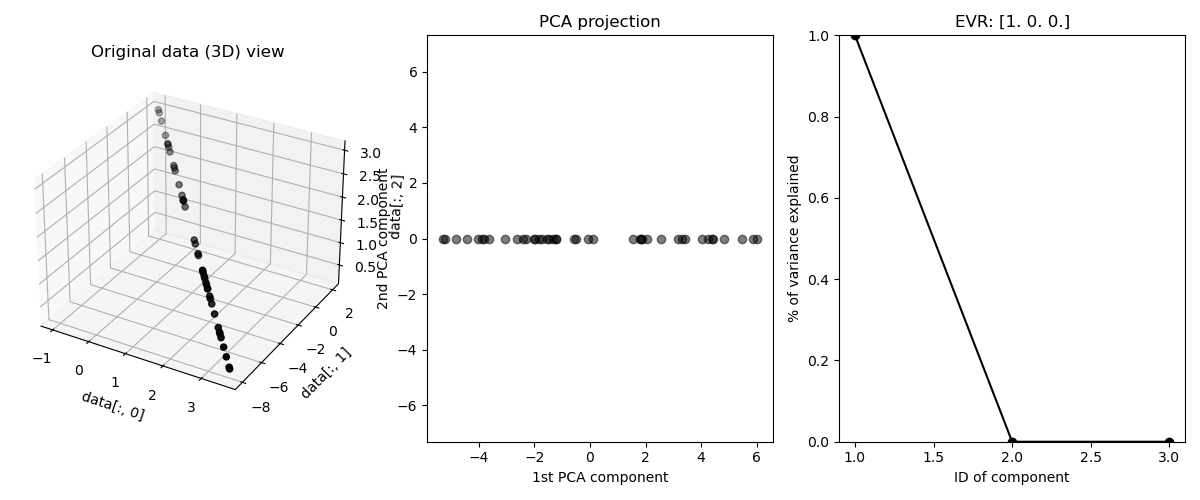
\includegraphics[width=0.9\textwidth]{images/pca/Line.png}\end{center}\end{frame}
\begin{frame}\frametitle{Analiza składowych głównych -- przykład/idea działania}
\begin{center}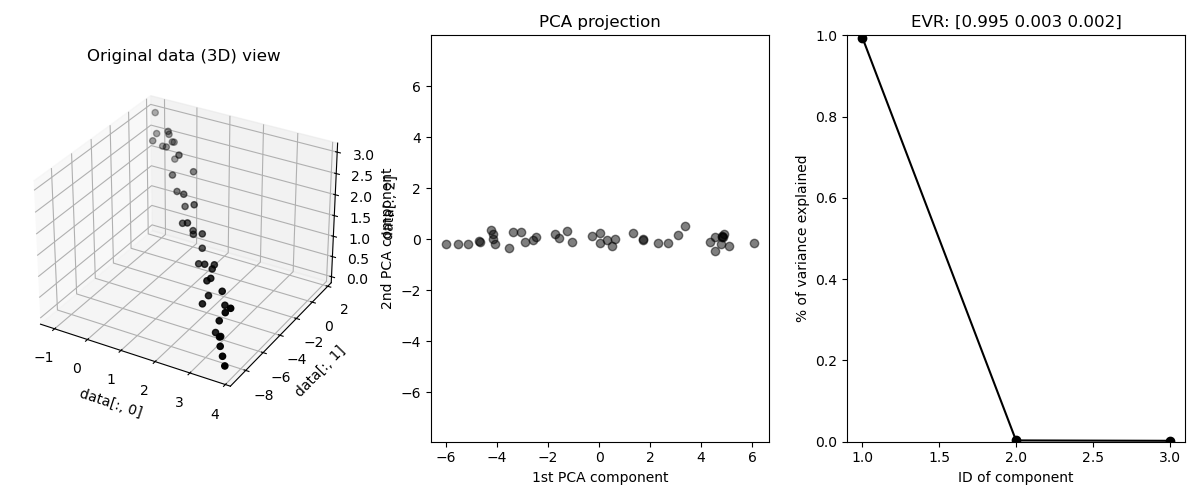
\includegraphics[width=0.9\textwidth]{images/pca/Line,_noise0.2.png}\end{center}\end{frame}
\begin{frame}\frametitle{Analiza składowych głównych -- przykład/idea działania}
\begin{center}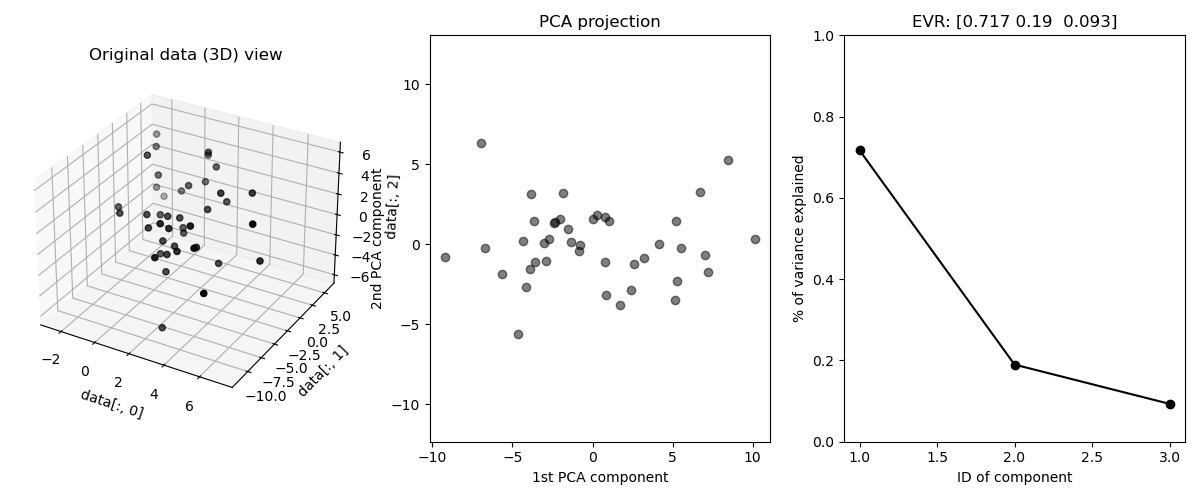
\includegraphics[width=0.9\textwidth]{images/pca/Line,_noise2.png}\end{center}\end{frame}
\begin{frame}\frametitle{Analiza składowych głównych -- przykład/idea działania}
\begin{center}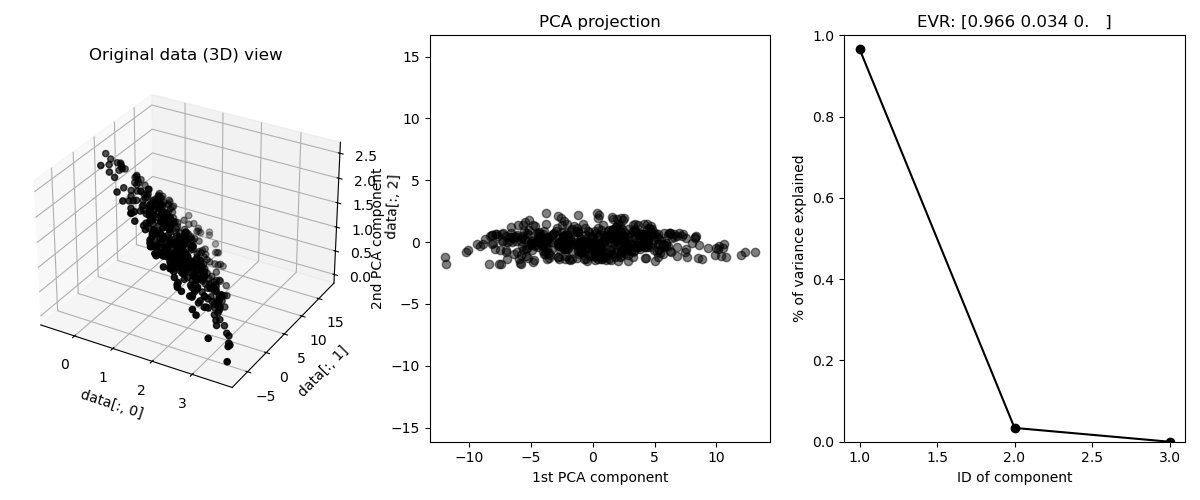
\includegraphics[width=0.9\textwidth]{images/pca/Triangle.png}\end{center}\end{frame}
\begin{frame}\frametitle{Analiza składowych głównych -- przykład/idea działania}
\begin{center}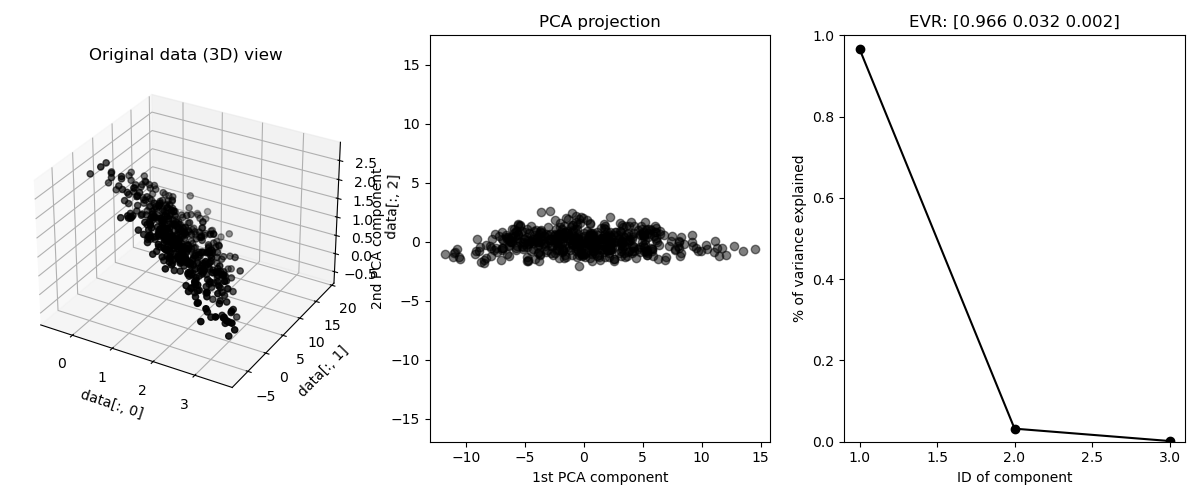
\includegraphics[width=0.9\textwidth]{images/pca/Triangle,_noise0.2.png}\end{center}\end{frame}
\begin{frame}\frametitle{Analiza składowych głównych -- przykład/idea działania}
\begin{center}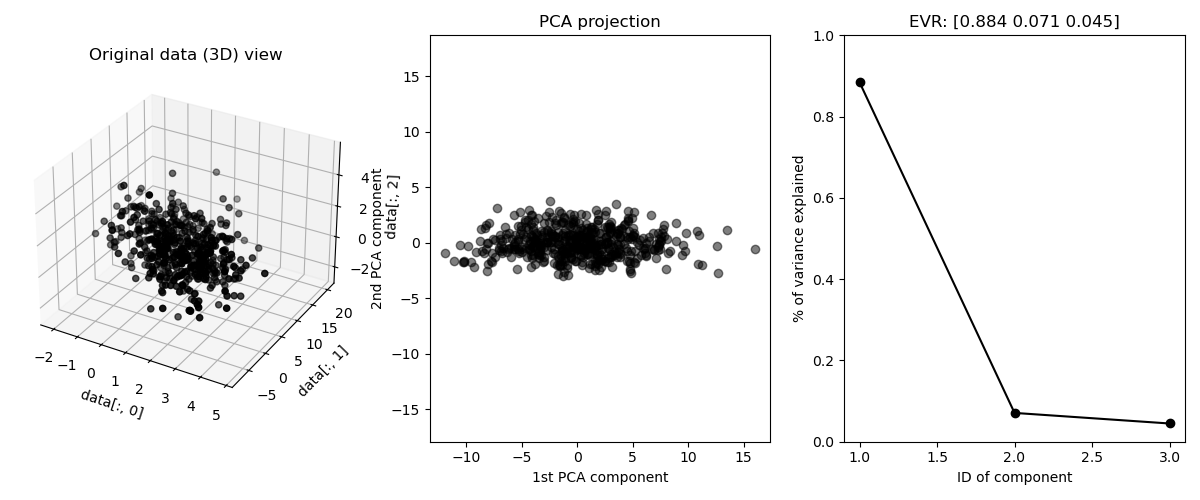
\includegraphics[width=0.9\textwidth]{images/pca/Triangle,_noise1.png}\end{center}\end{frame}
\begin{frame}\frametitle{Analiza składowych głównych -- przykład/idea działania}
\begin{center}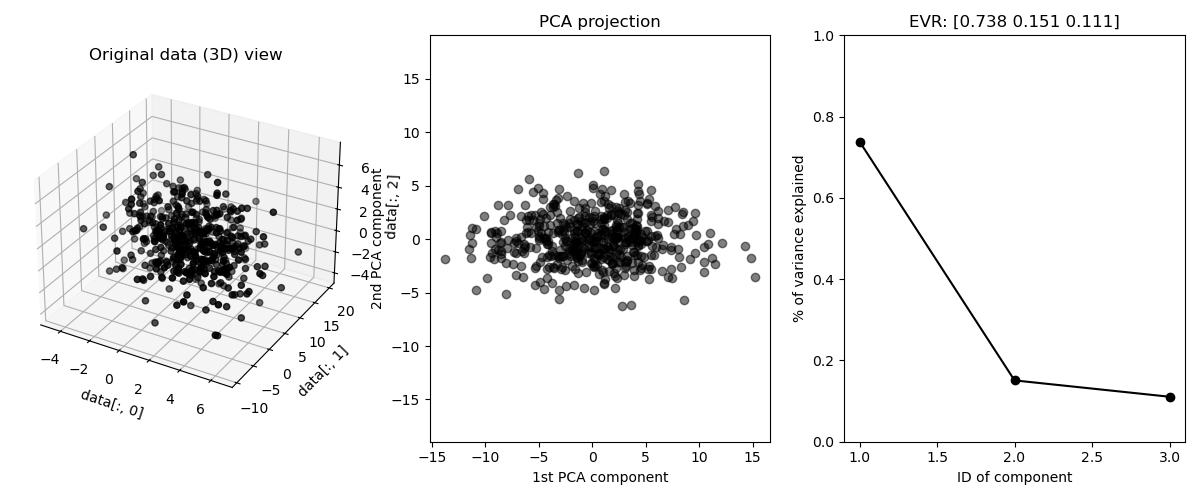
\includegraphics[width=0.9\textwidth]{images/pca/Triangle,_noise2.png}\end{center}\end{frame}
\begin{frame}\frametitle{Analiza składowych głównych -- przykład/idea działania}
\begin{center}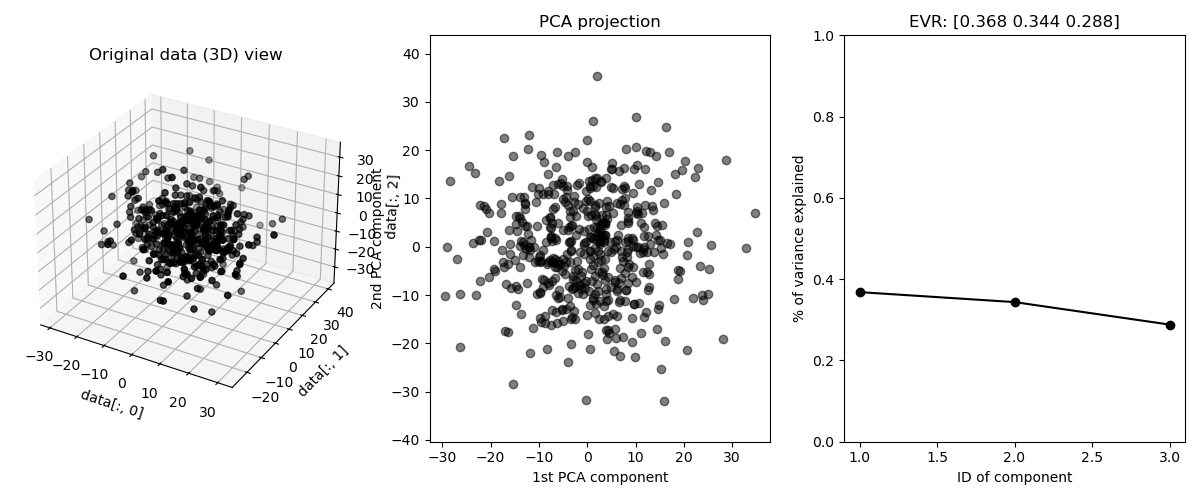
\includegraphics[width=0.9\textwidth]{images/pca/Triangle,_noise10.png}\end{center}\end{frame}
\begin{frame}\frametitle{Analiza składowych głównych -- przykład (wybielenie -- whitening)}
\begin{center}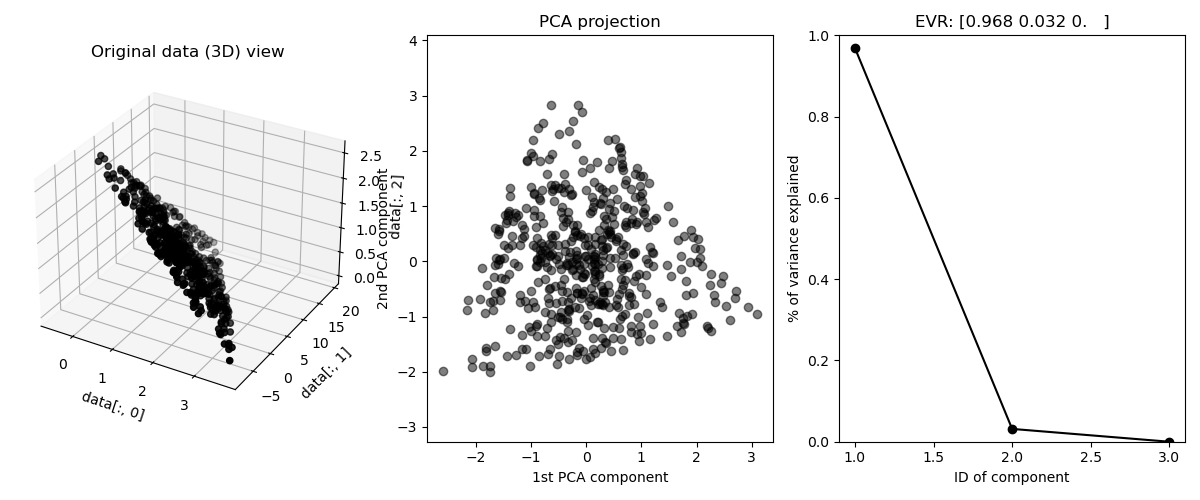
\includegraphics[width=0.9\textwidth]{images/pca/Triangle_(whitened).png}\end{center}\end{frame}

\begin{frame}
	\frametitle{Analiza składowych głównych -- przykład zastosowania (reprezentacja)}
	\begin{itemize}
		\item $x$ to zlinearyzowany obraz ($x\in\mathbb{R}^{4096}$):\\
		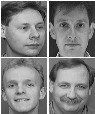
\includegraphics[width=0.1\textwidth]{images/olivettifaces.jpg}\hspace*{0.5cm}
		\begin{tabular}{c|c}
			$\mathbf{x}_1$ & $\mathbf{x}_2$ \\\hline $\mathbf{x}_3$ & $\mathbf{x}_4$
		\end{tabular}\pause
		\item Składowe (wektory z macierzy $A$) tzw. ,,eigenfaces''\\
		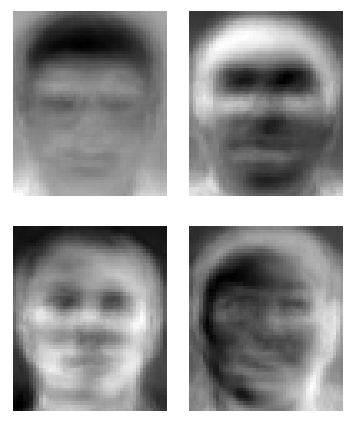
\includegraphics[width=0.1\textwidth]{images/Eigenfaces.png}\\\pause
		\dots cechy twarzy
	\end{itemize}
\end{frame}

\begin{frame}
	\frametitle{Analiza składowych głównych -- przykład zastosowania (reprezentacja)}
	\begin{itemize}
		\item $\mathbf{x}\in\mathbb{R}^{4096}\rightarrow \mathbf{c}\in\mathbb{R}^{4096}$?\pause
		\begin{itemize}
			\item Macierz kowariancji $S= \frac{1}{m-1}X X^\top$\pause
			\item Wektory własne ($\rightarrow A$) oraz wartości własne (wariancja, posortowane)\pause
			\item Można wykorzystać pierwszych $n$ wektorów -- $\mathbf{x}\in\mathbb{R}^{4096}\rightarrow \mathbf{c}\in\mathbb{R}^{n}$; np. $n=5, 10, 50$\pause
		\end{itemize}
		\item Rekonstrukcja z 1, 9, 17, \dots (+8 składowych):
		\begin{center}
			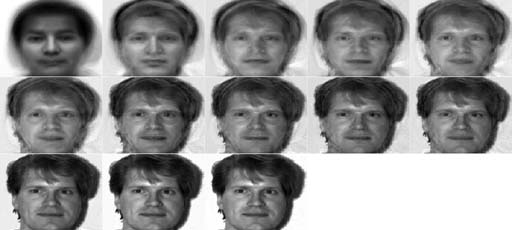
\includegraphics[width=0.5\textwidth]{images/pca-reconstruction.png}
			%\attr{Turk and Pentland}
		\end{center}
	\end{itemize}
\end{frame}

\begin{frame}
	\frametitle{Analiza składowych głównych -- przykład zastosowania (analiza)}
	\begin{center}
	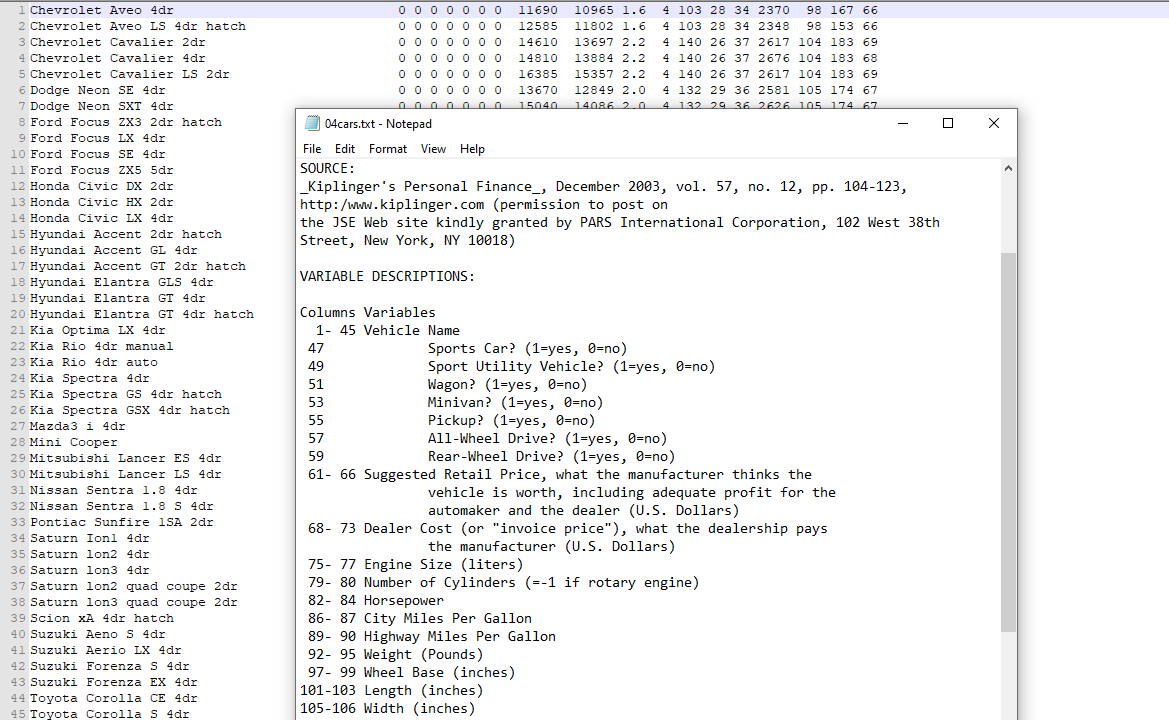
\includegraphics[width=0.7\textwidth]{images/cars/dataset.png}
	\end{center}
\end{frame}

\begin{frame}
	\frametitle{Analiza składowych głównych -- przykład zastosowania (analiza)}
	\begin{center}
		\includegraphics[width=0.9\textwidth]{images/cars/cars.png}
	\end{center}
\end{frame}

\begin{frame}
	\frametitle{Analiza składowych głównych -- przykład zastosowania (analiza)}
	\begin{center}
		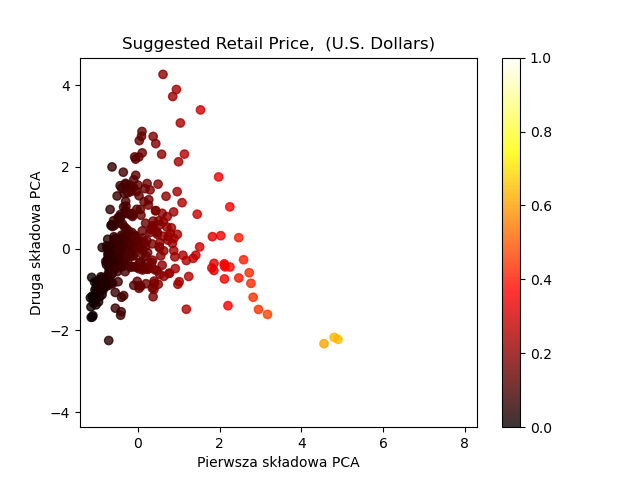
\includegraphics[width=0.56\textwidth]{images/cars/pric.png}
	\end{center}
\end{frame}
\begin{frame}
	\frametitle{Analiza składowych głównych -- przykład zastosowania (analiza)}
	\begin{center}
		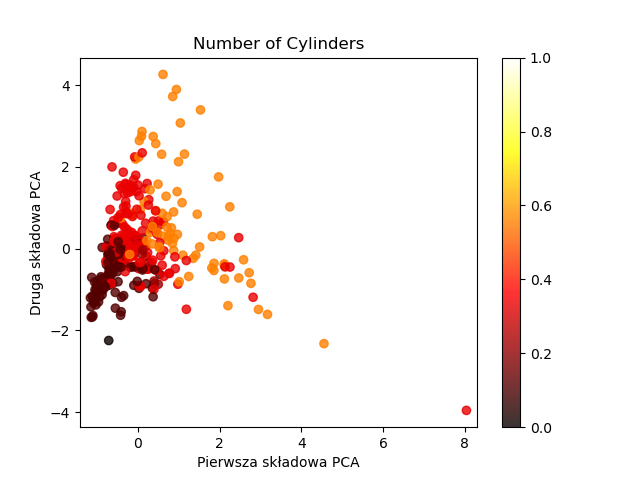
\includegraphics[width=0.56\textwidth]{images/cars/cyls.png}
	\end{center}
\end{frame}
\begin{frame}
	\frametitle{Analiza składowych głównych -- przykład zastosowania (analiza)}
	\begin{center}
		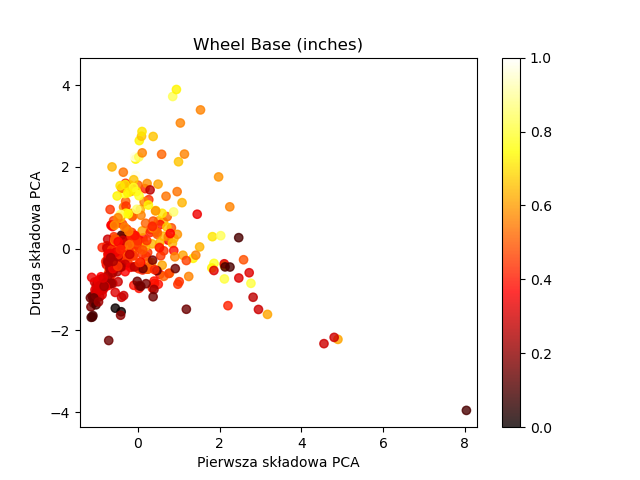
\includegraphics[width=0.56\textwidth]{images/cars/wheel.png}
	\end{center}
\end{frame}
\begin{frame}[fragile]
	\frametitle{Analiza składowych głównych -- przykład zastosowania (analiza)}
	\small
	\begin{verbatim}
		Component 0 ---------------------------
		
		Examples
		Lowest
		['Kia Rio 4dr manual' 'Hyundai Accent 2dr hatch' 'Toyota Echo 2dr manual']
		Highest
		['Mercedes-Benz SL600 convertible 2dr' 'Mercedes-Benz CL600 2dr'
		'Porsche 911 GT2 2dr']
		
		Column correlations
		07 1.00  61- 66 Suggested Retail Price, what the manufacturer thinks the vehicle 
		is worth, including adequate profit for the automaker and the dealer (U.S. Dollars)
		08 1.00  68- 73 Dealer Cost (or "invoice price"), what the dealership pays              the manufacturer (U.S. Dollars)
	\end{verbatim}
\end{frame}
\begin{frame}[fragile]
	\frametitle{Analiza składowych głównych -- przykład zastosowania (analiza)}
	\small
	\begin{verbatim}
		Component 1 ---------------------------
		
		Examples
		Lowest
		['Porsche 911 GT2 2dr' 'Mercedes-Benz SL55 AMG 2dr'
		'Honda Insight 2dr (gas/electric)']
		Highest
		['Hummer H2' 'Lincoln Navigator Luxury' 'GMC Yukon XL 2500 SLT']
		
		Column correlations
		14 0.83  92- 95 Weight (Pounds)
		17 0.74 105-106 Width (inches)
		
	\end{verbatim}
\end{frame}
\begin{frame}[fragile]
	\frametitle{Analiza składowych głównych -- przykład zastosowania (analiza)}
	\small
	\begin{verbatim}
		Component 4 ---------------------------
		
		Examples
		Lowest
		['Lincoln Town Car Ultimate L 4dr' 'Chrysler Concorde LX 4dr'
		'Lincoln Town Car Ultimate 4dr']
		Highest
		['Mini Cooper S' 'Hummer H2' 'Jeep Wrangler Sahara convertible 2dr']
		
		Column correlations
		16 0.74 101-103 Length (inches)
		15 0.51  97- 99 Wheel Base (inches)
	\end{verbatim}
\end{frame}
\begin{frame}
	\frametitle{Analiza składowych głównych -- przykład zastosowania (analiza)}
	\begin{center}
		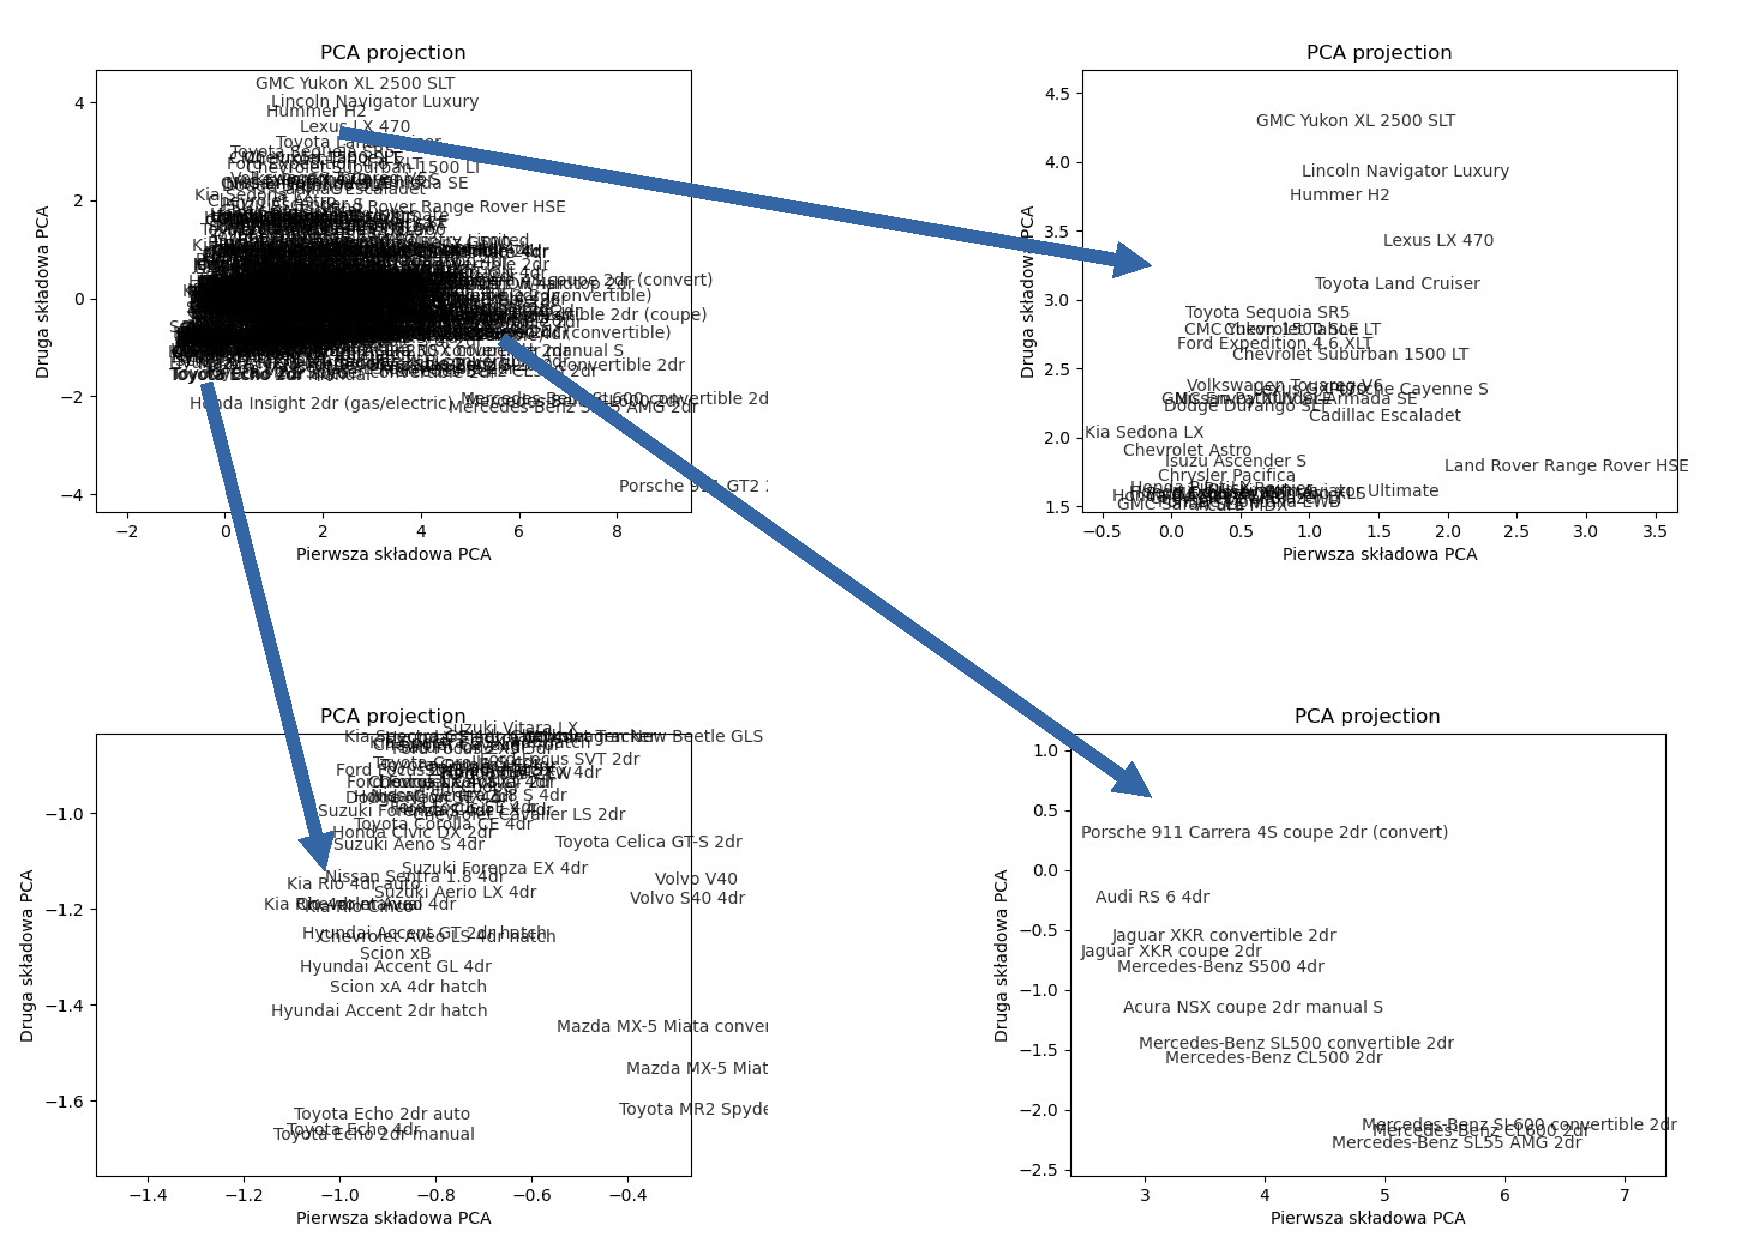
\includegraphics[width=0.6\textwidth]{images/cars/cmalle.pdf}
	\end{center}
\end{frame}

\begin{frame}
	\frametitle{Analiza składowych głównych -- podsumowanie}
	\begin{enumerate}
		\item Reprezentacja $x$ uwzględniająca charakterystykę źródła danych\pause
		\begin{itemize}
			\item Mniej współczynników do reprezentacji i klasyfikacji\pause
			\item Podzbiór współczynników zachowuje zakres zmienności danych
			\item Analiza zbioru danych -- data mining -- weryfikacja obecności grup, anomalii, outlierów
		\end{itemize}
	\end{enumerate}
\end{frame}


\subsection{Support Vector Machine}

\begin{frame}\begin{center}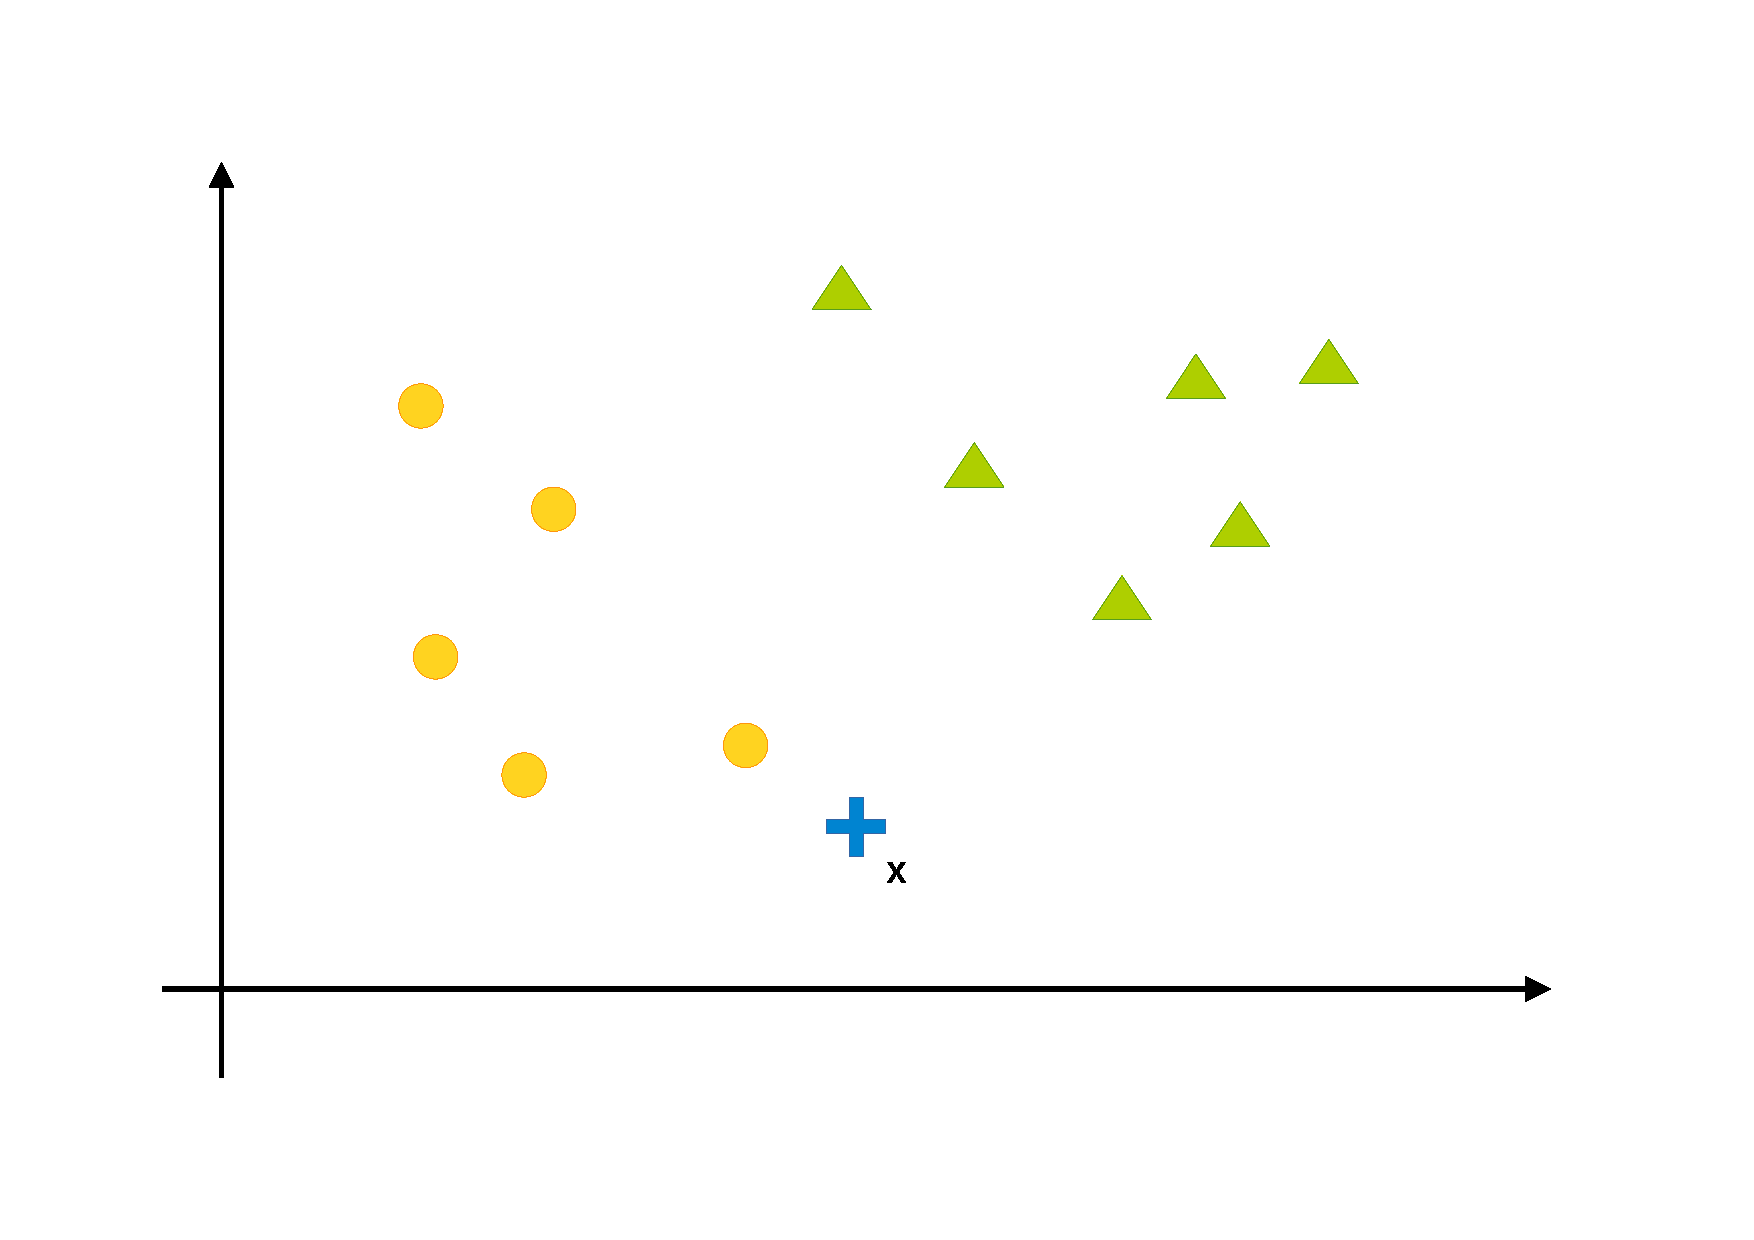
\includegraphics[width=0.7\textwidth]{images/svme.pdf}\end{center}\end{frame}
\begin{frame}\begin{center}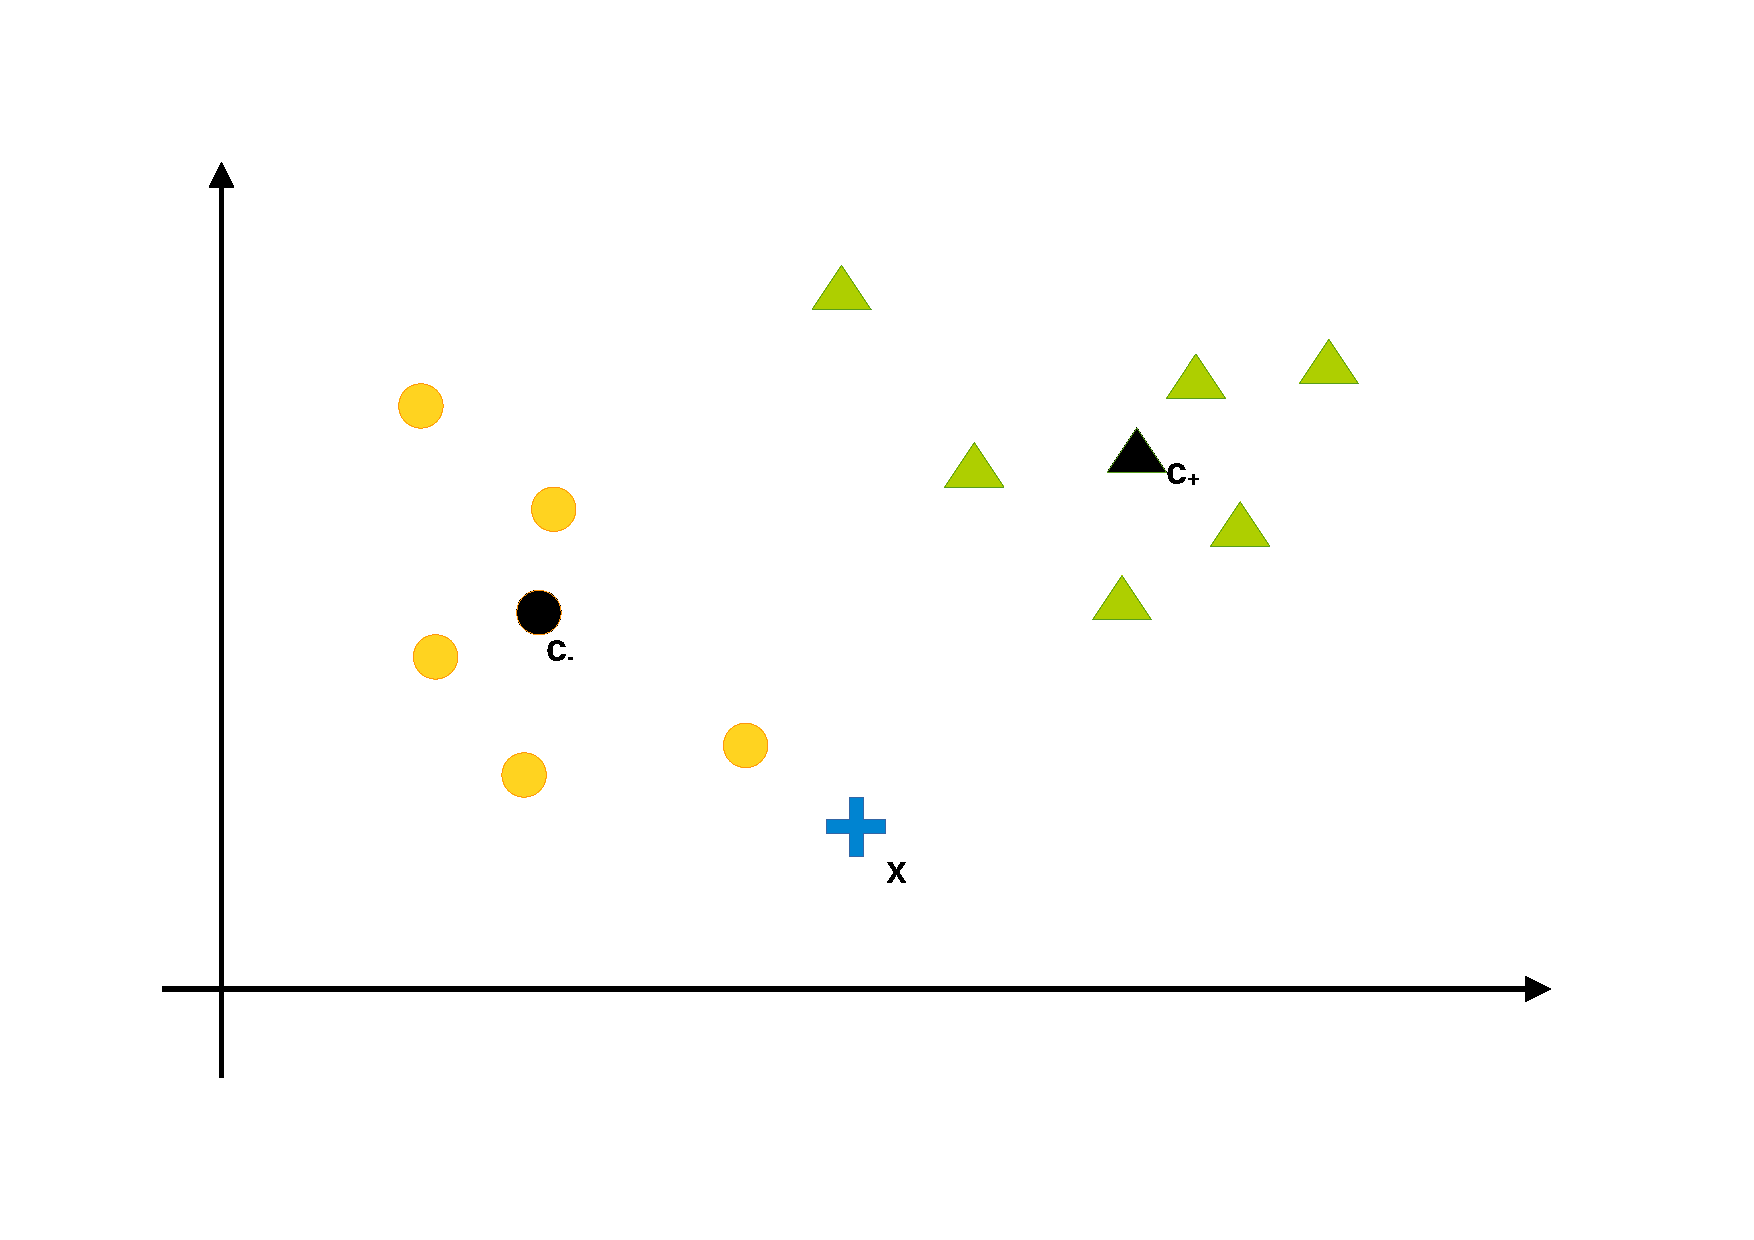
\includegraphics[width=0.7\textwidth]{images/svmd.pdf}\end{center}\end{frame}
\begin{frame}\begin{center}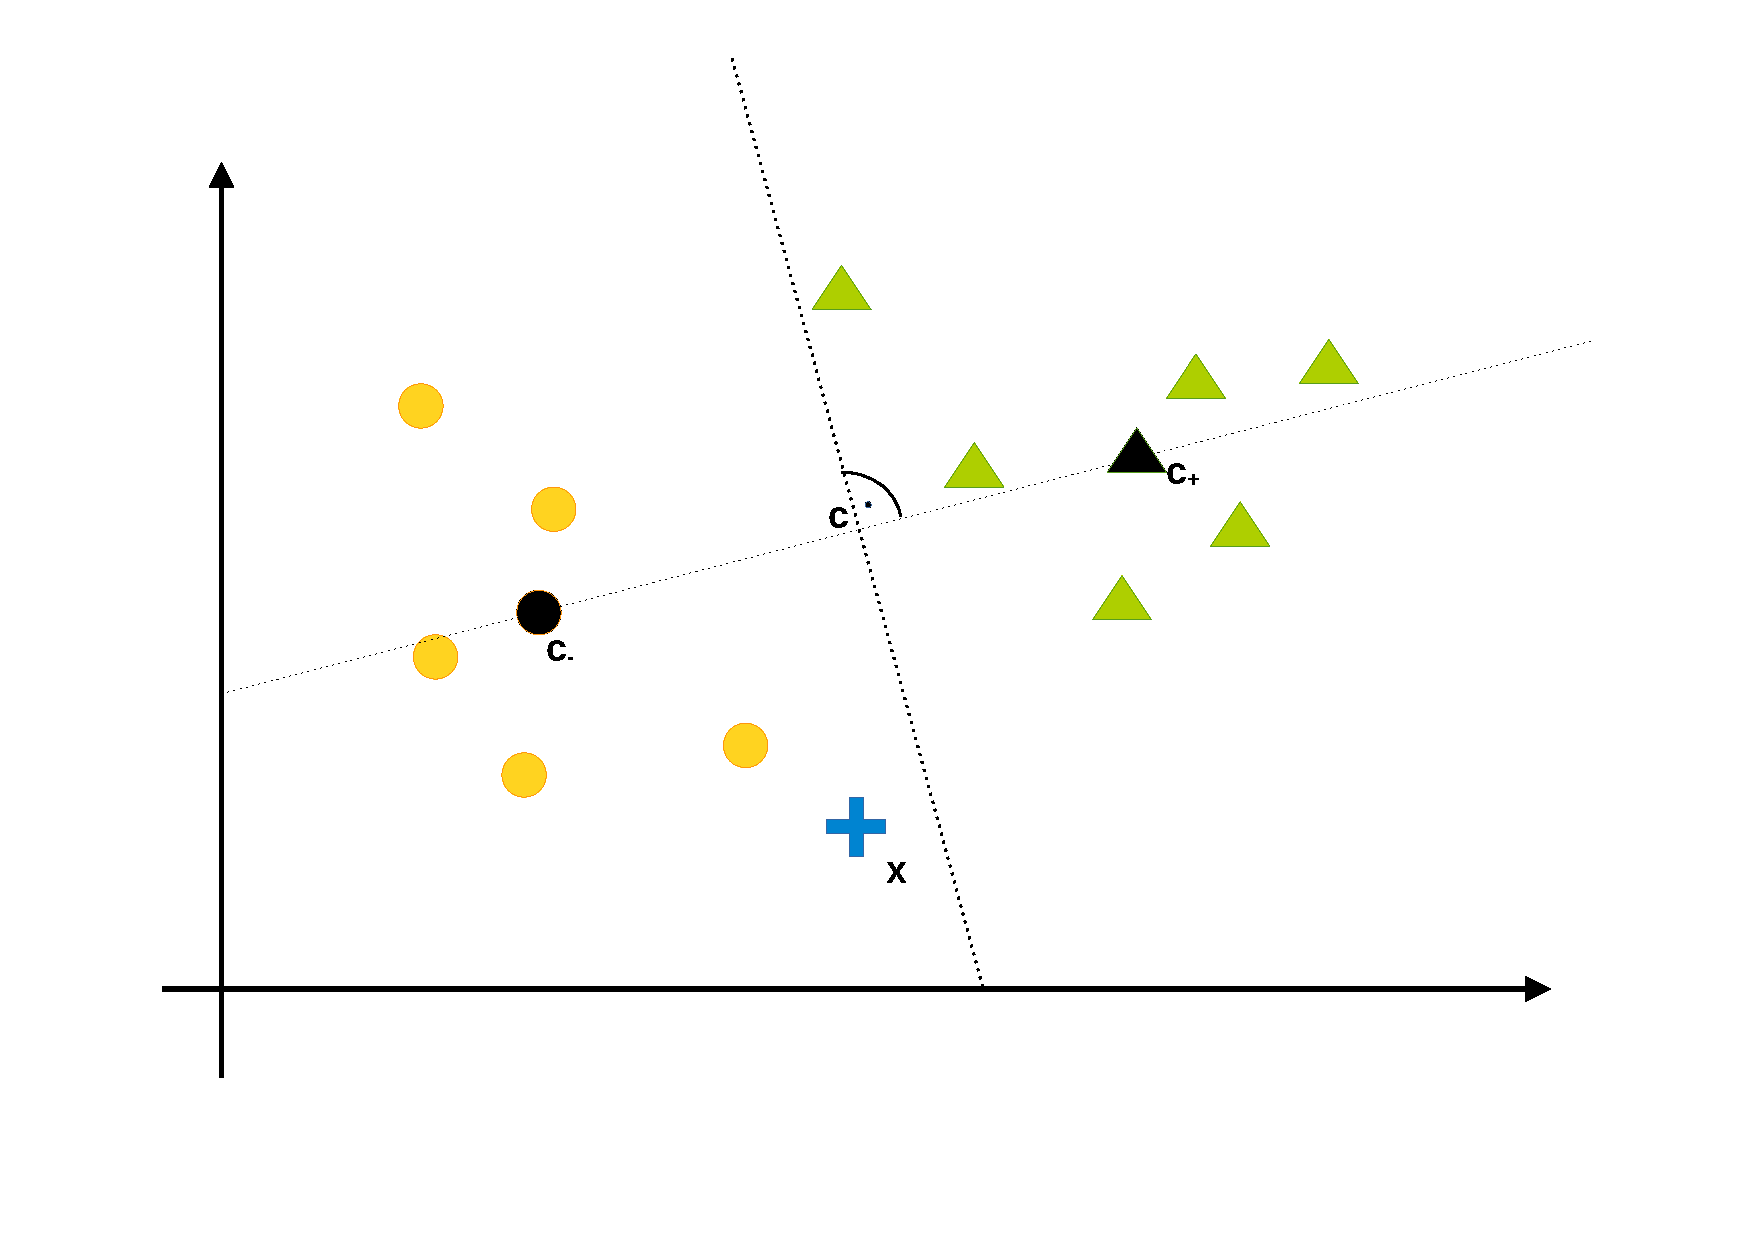
\includegraphics[width=0.7\textwidth]{images/svmc.pdf}\end{center}\end{frame}
\begin{frame}\begin{center}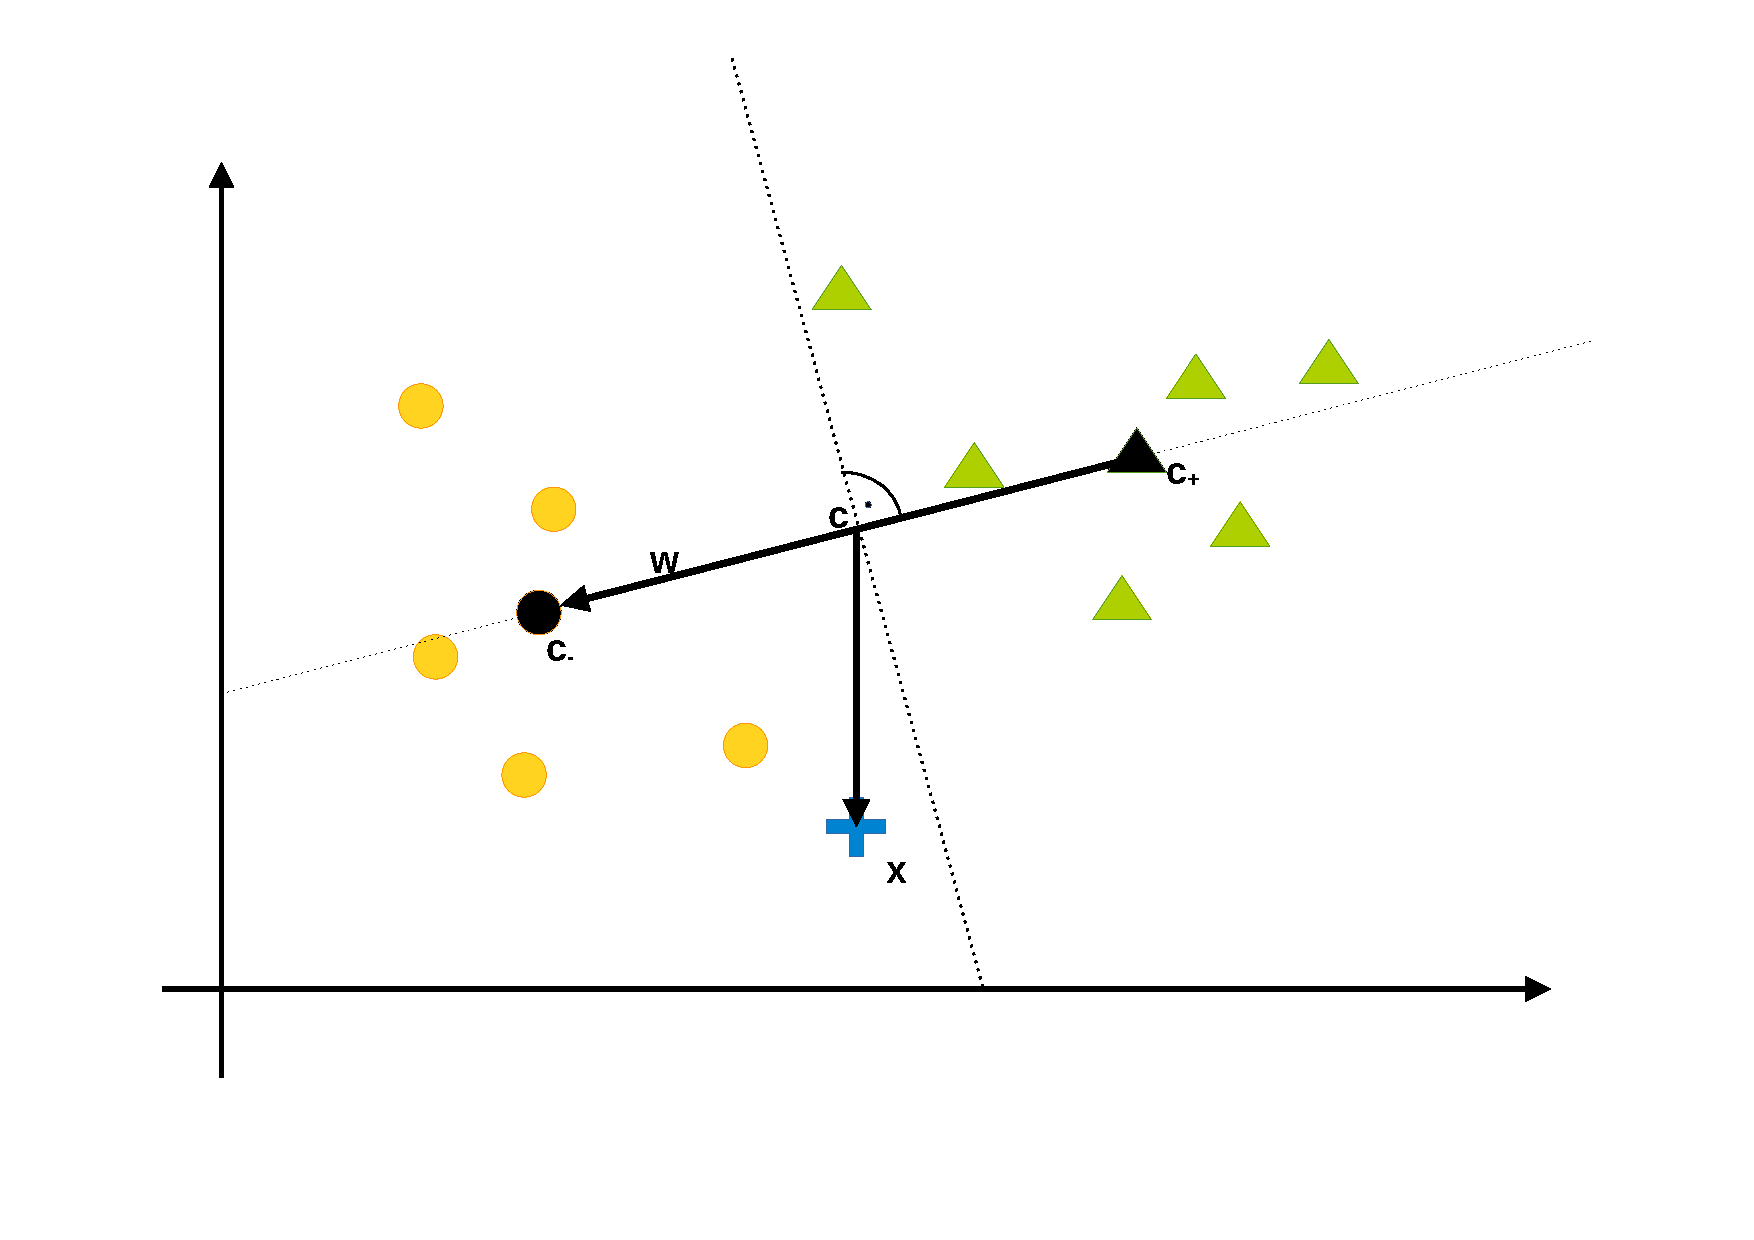
\includegraphics[width=0.7\textwidth]{images/svmb.pdf}\end{center}\end{frame}
\begin{frame}\begin{center}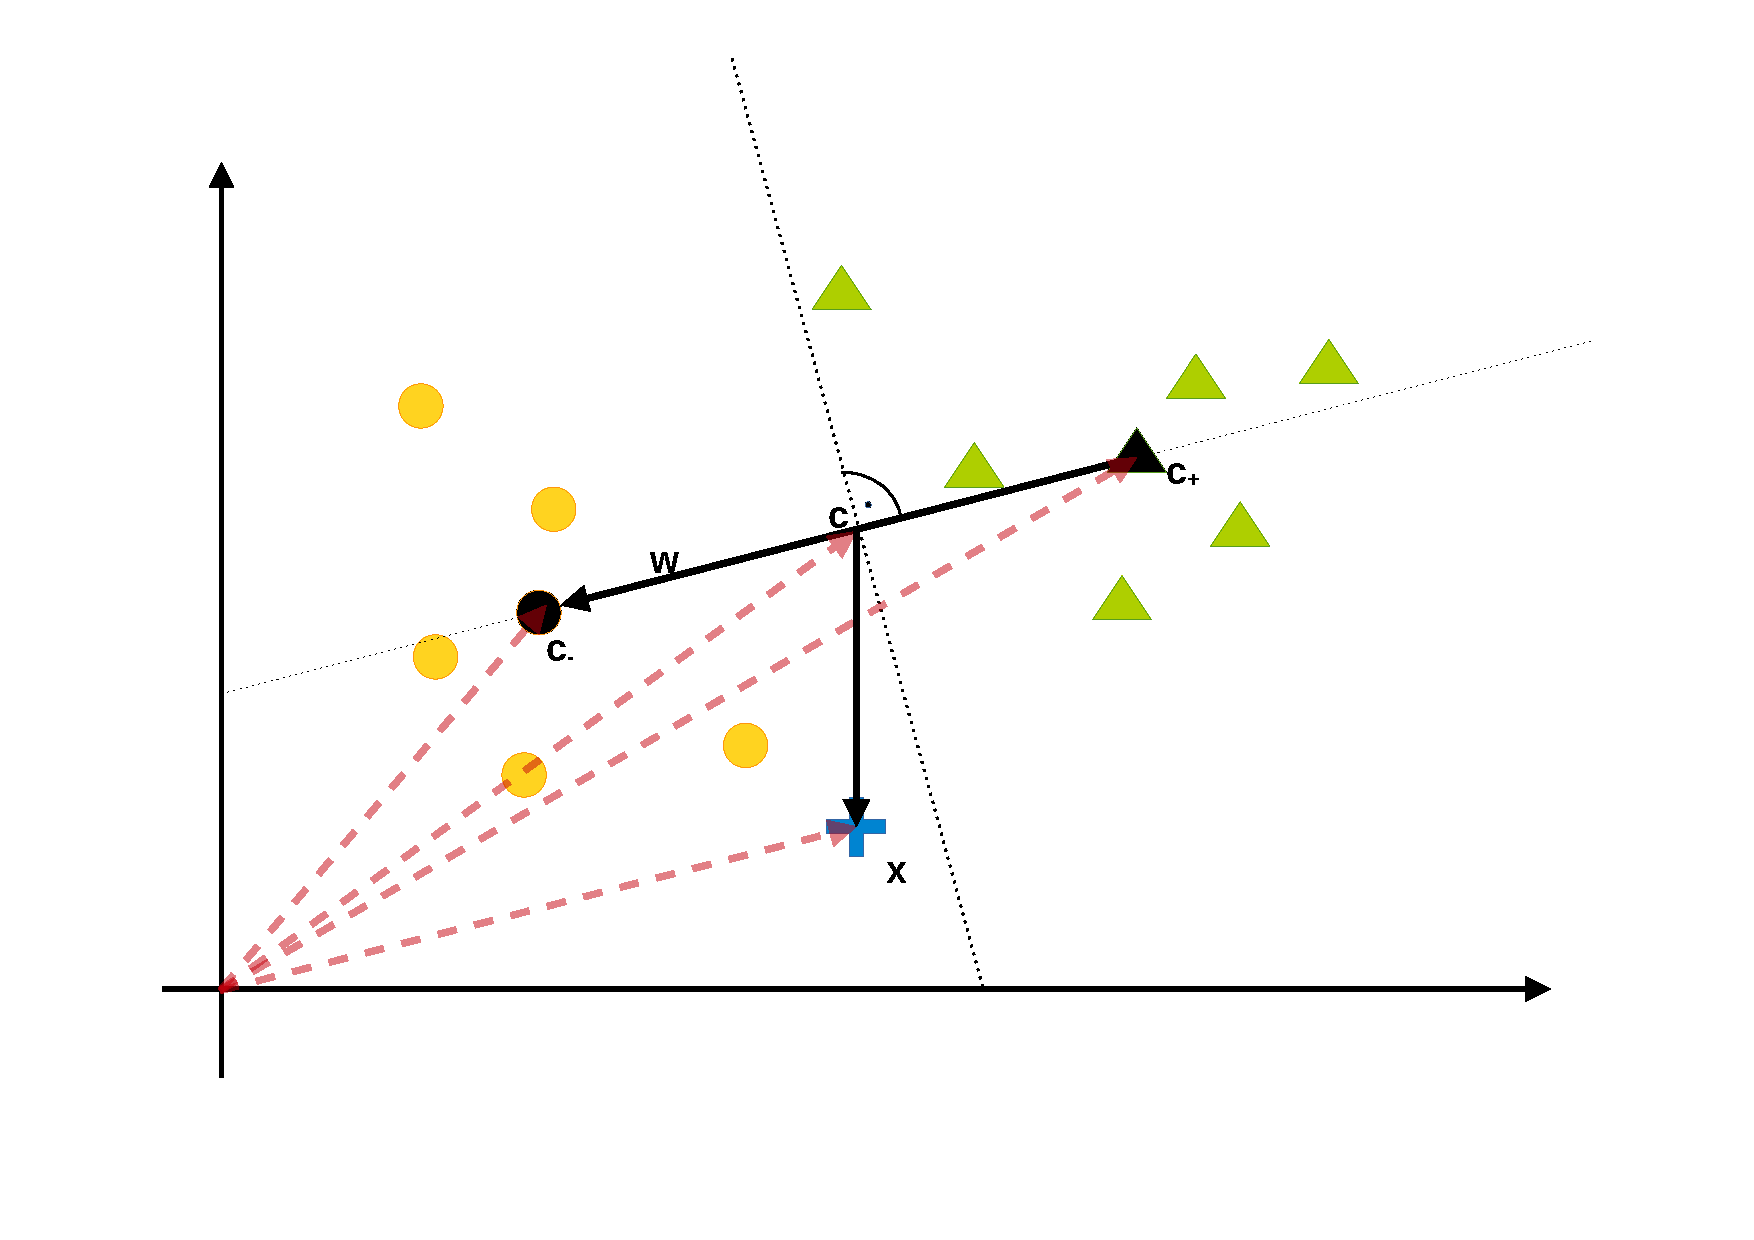
\includegraphics[width=0.7\textwidth]{images/svma.pdf}\end{center}\end{frame}
\begin{frame}\begin{center}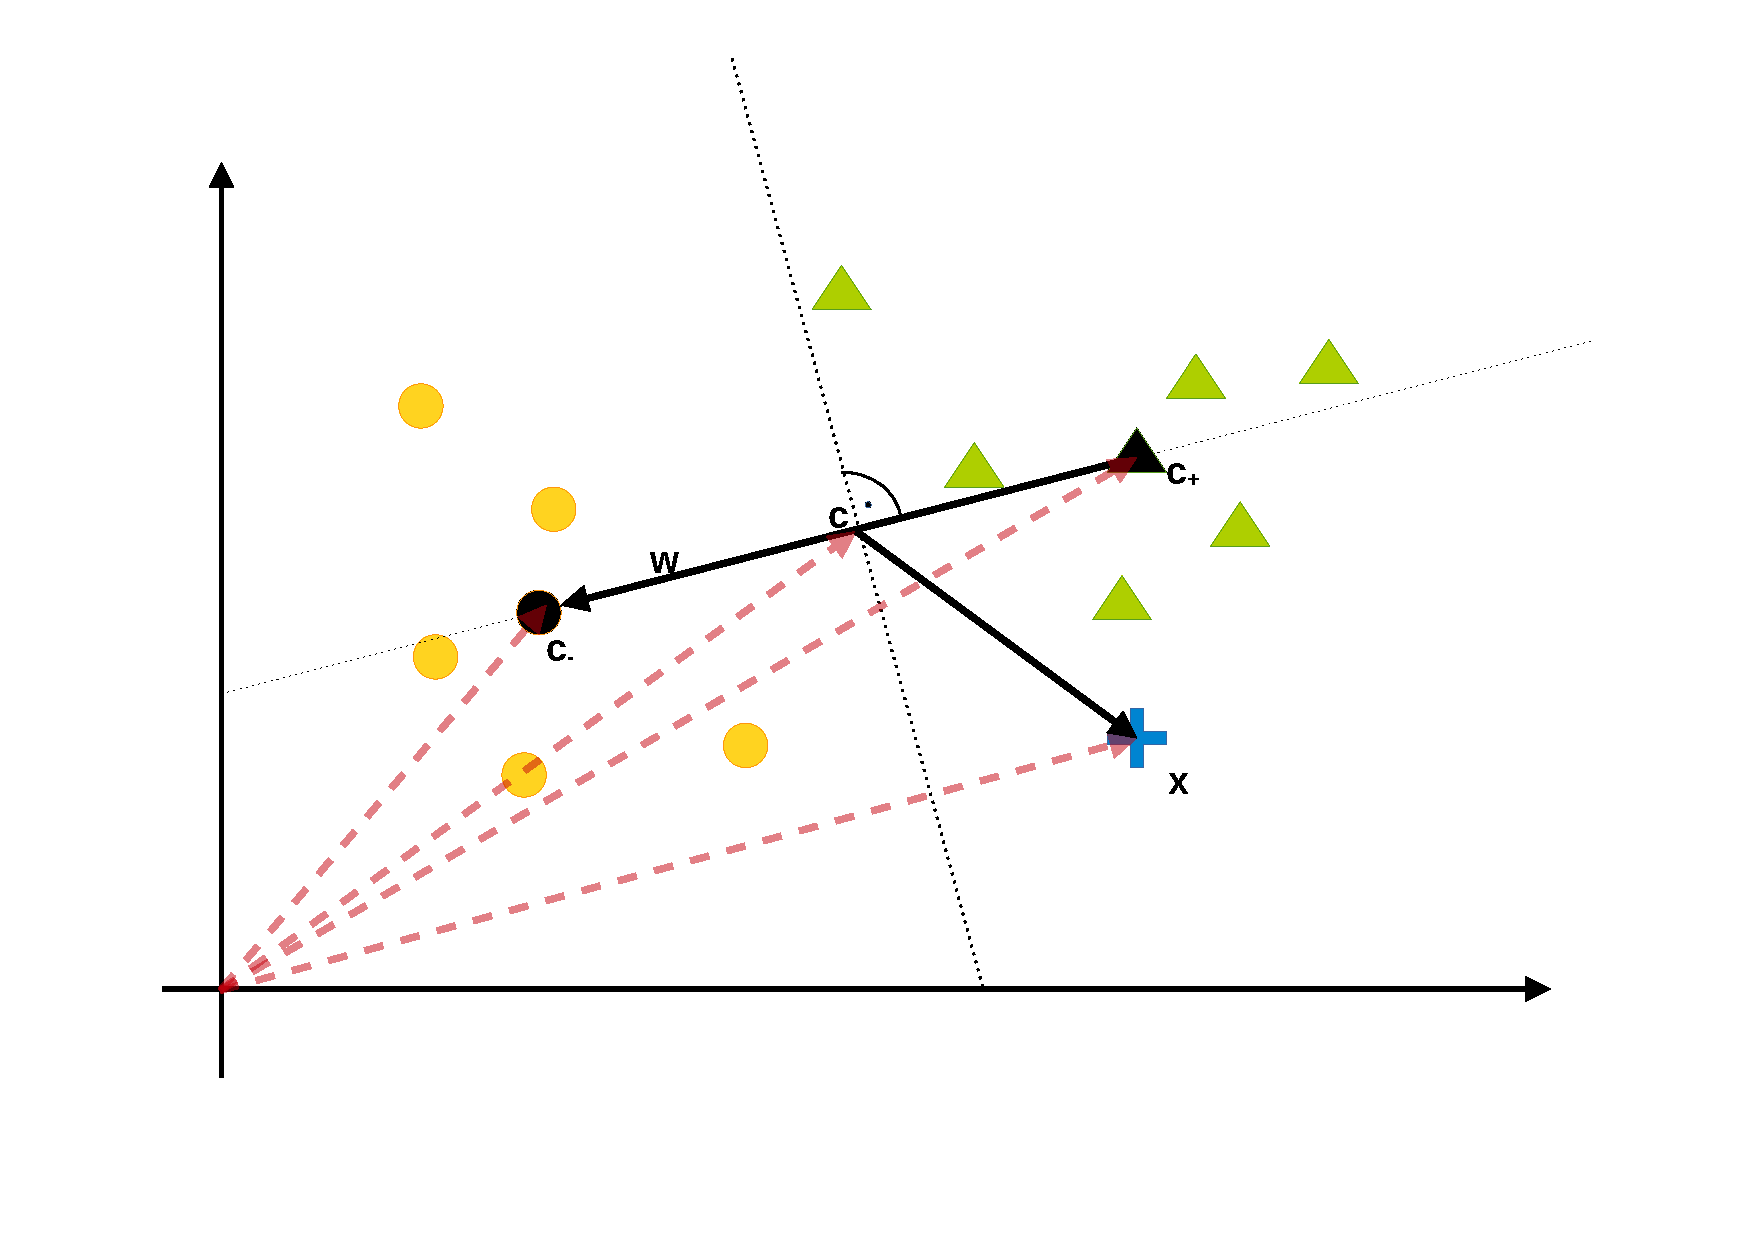
\includegraphics[width=0.7\textwidth]{images/svm1.pdf}\end{center}\end{frame}
\begin{frame}\begin{center}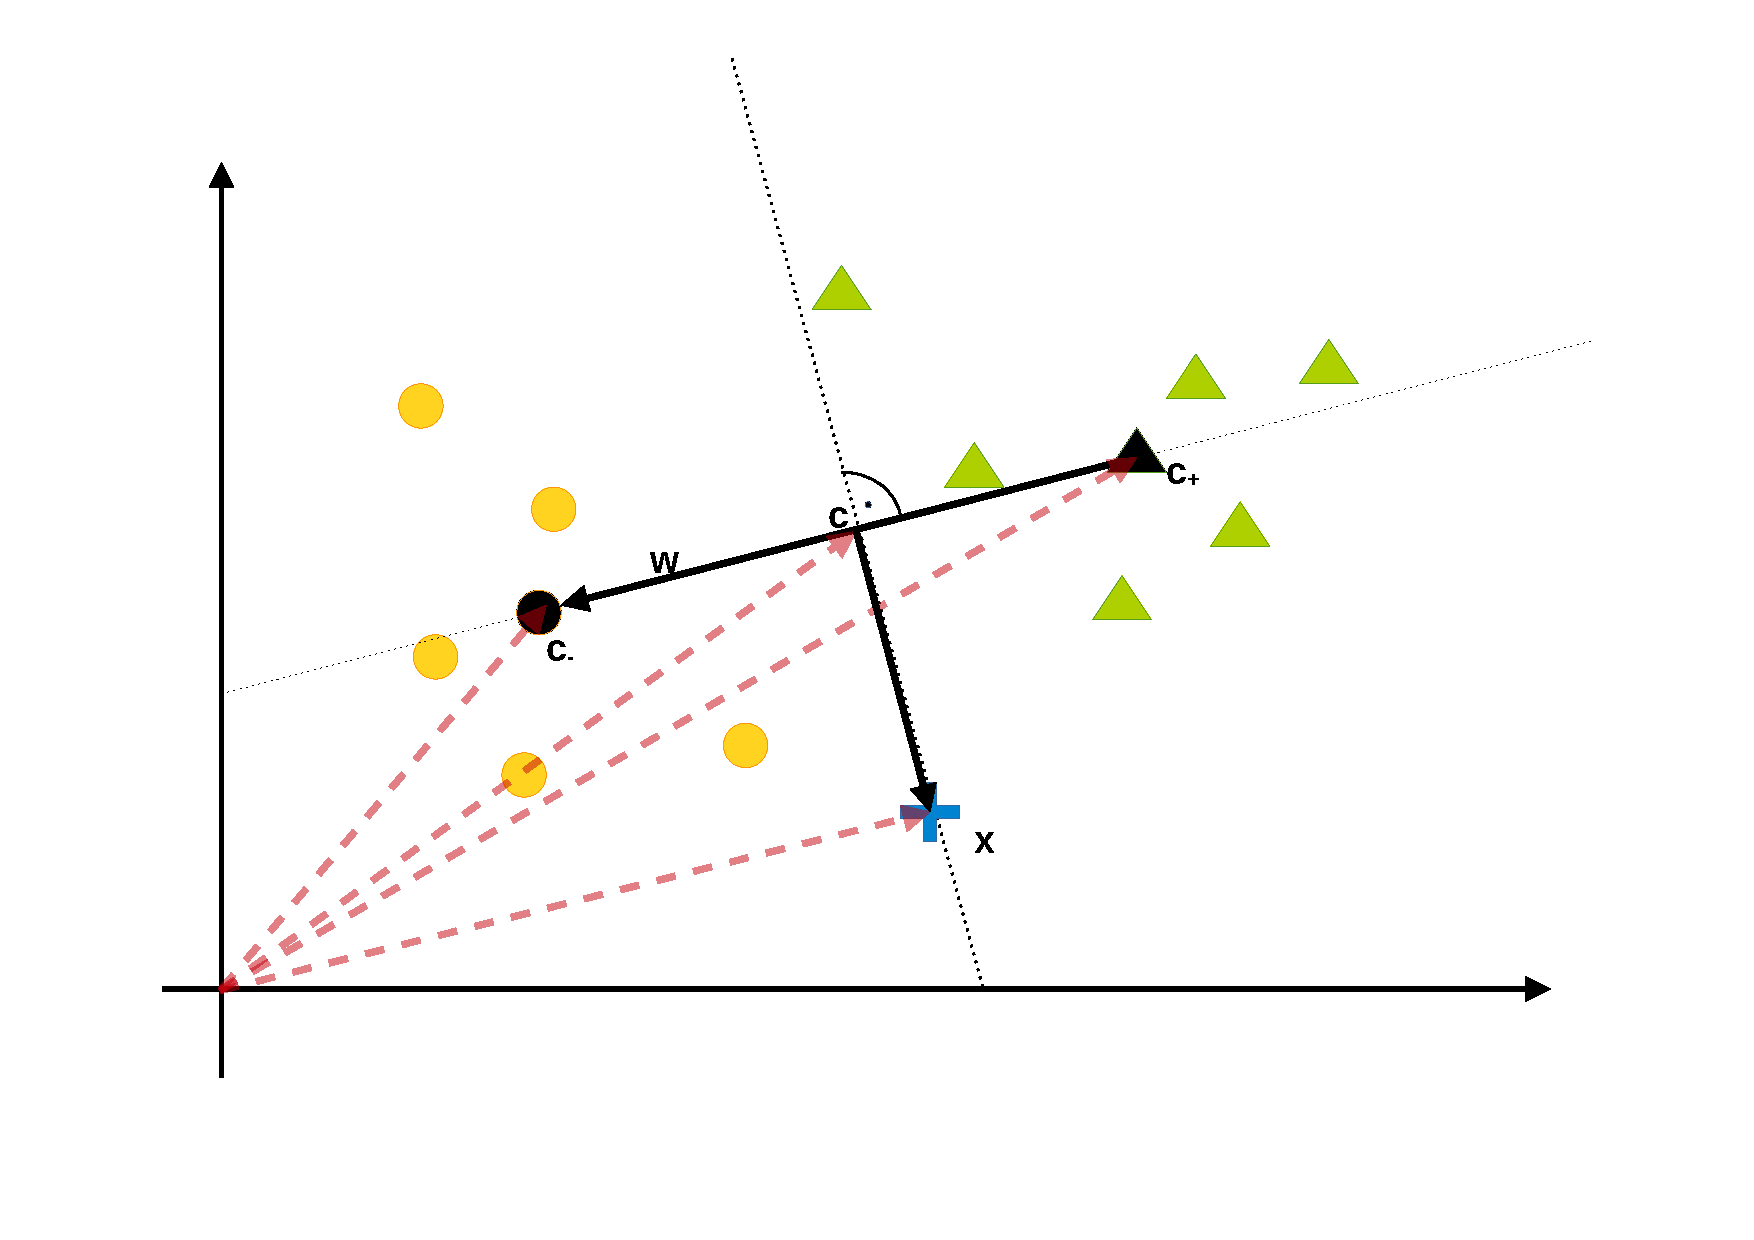
\includegraphics[width=0.7\textwidth]{images/svm0.pdf}\end{center}\end{frame}
\begin{frame}
	\begin{center}
		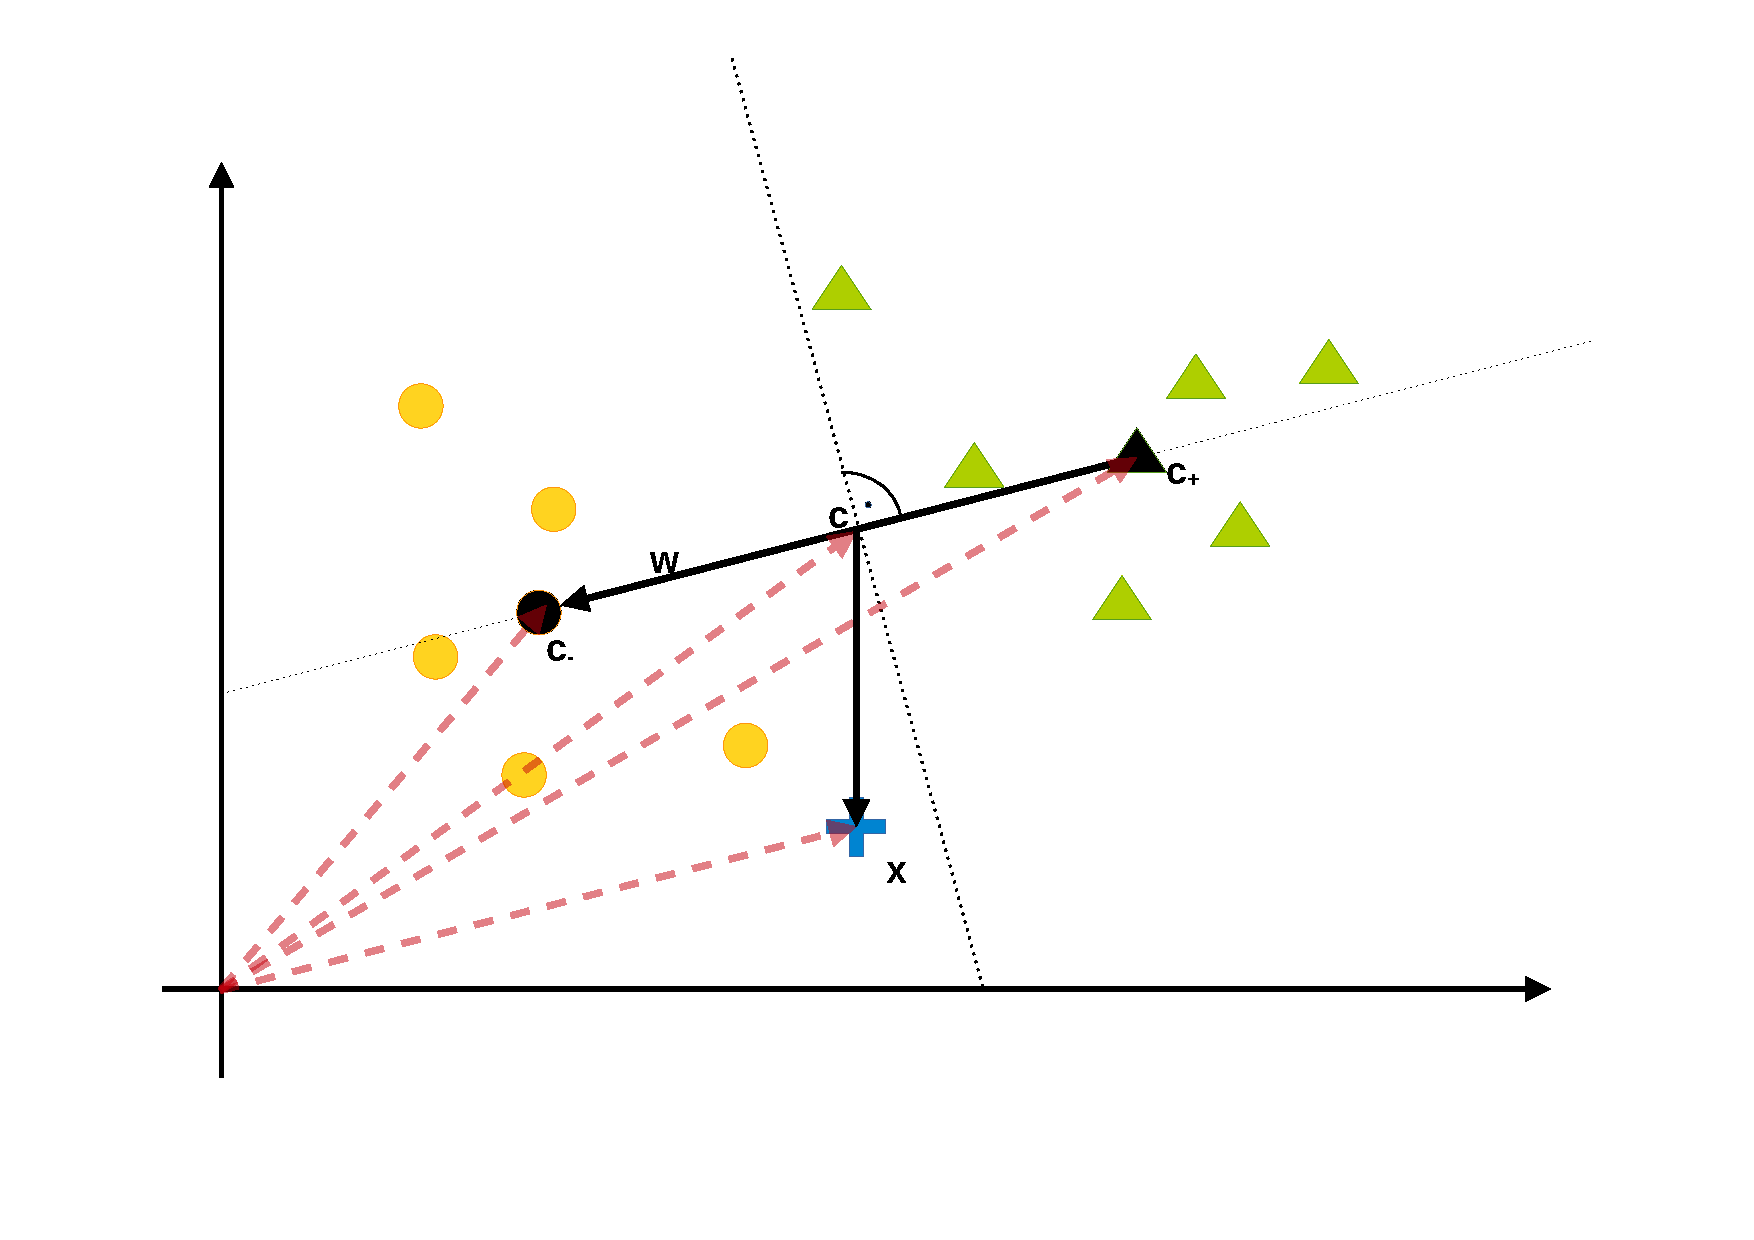
\includegraphics[width=0.3\textwidth]{images/svma.pdf}
		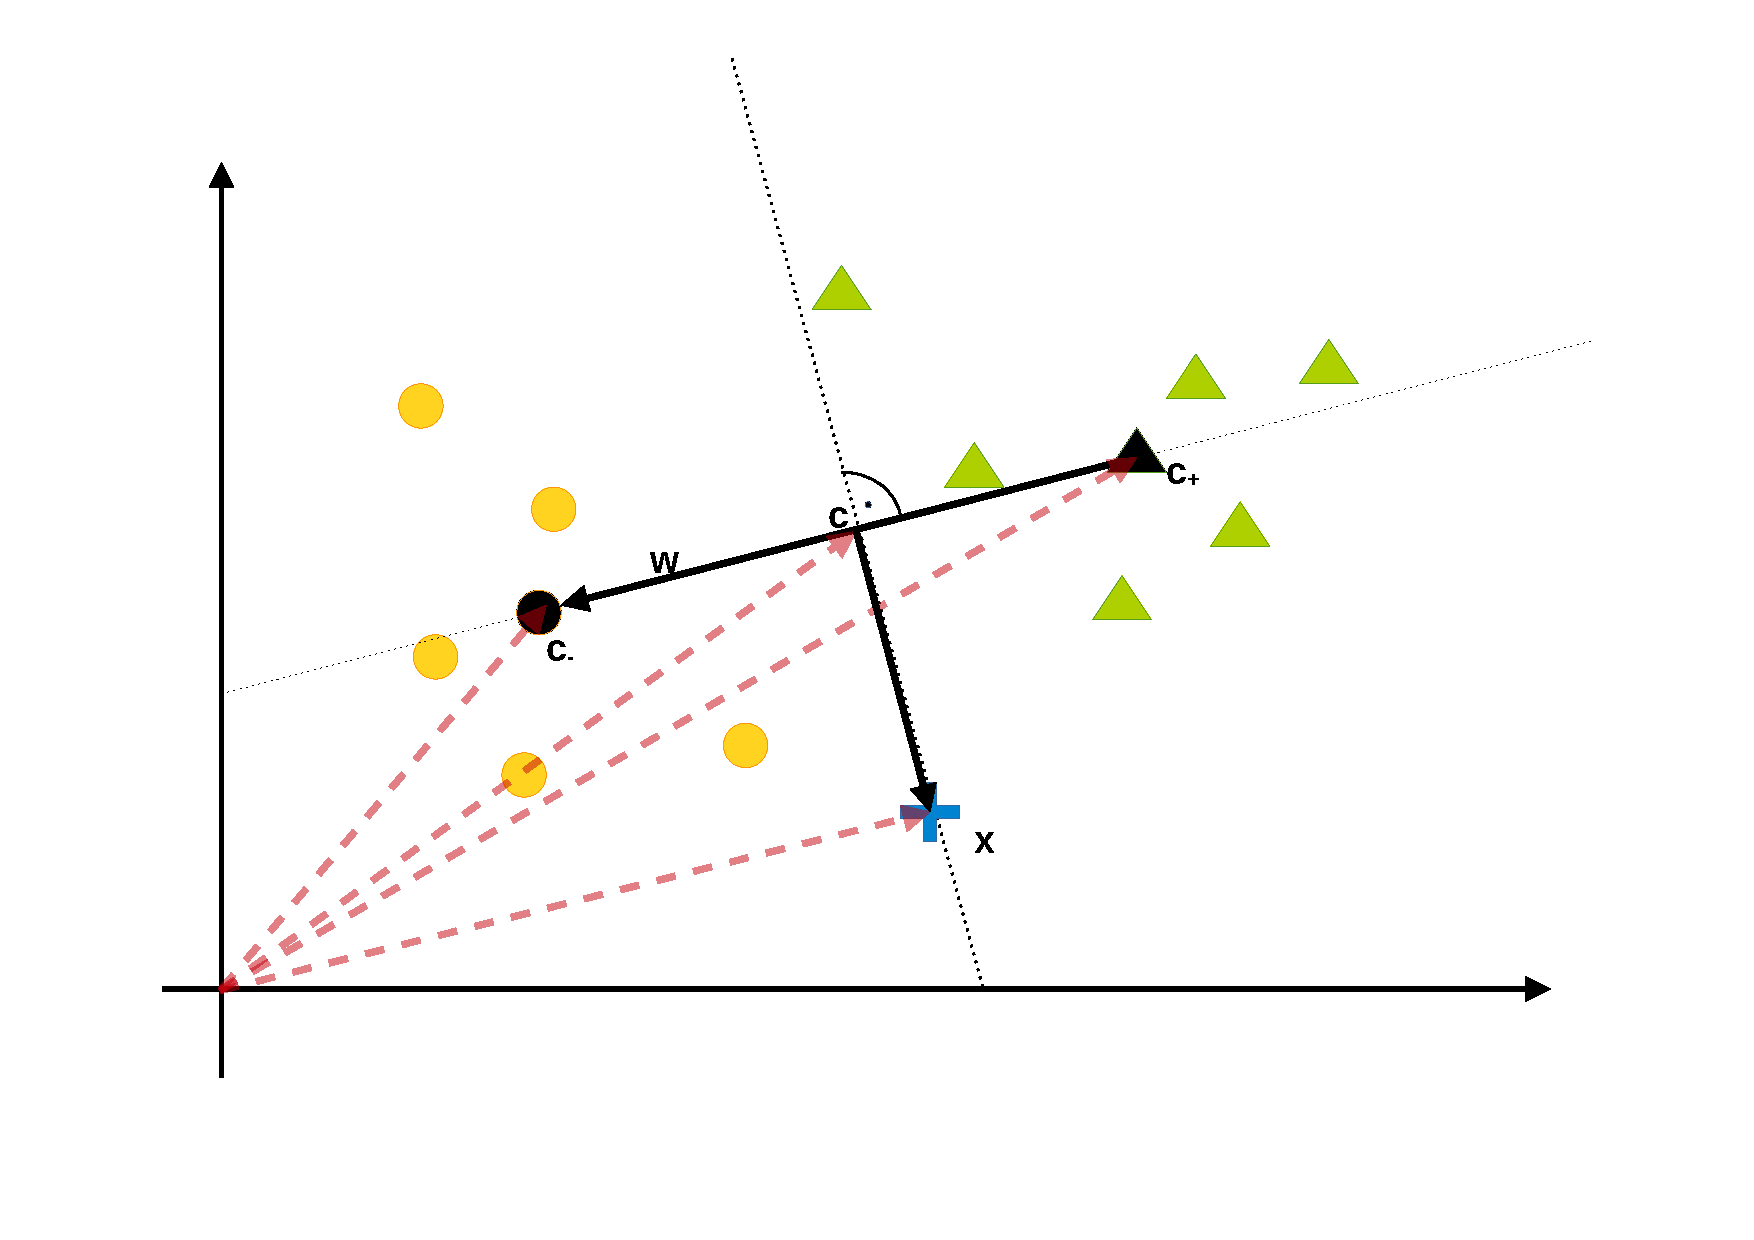
\includegraphics[width=0.3\textwidth]{images/svm0.pdf}
		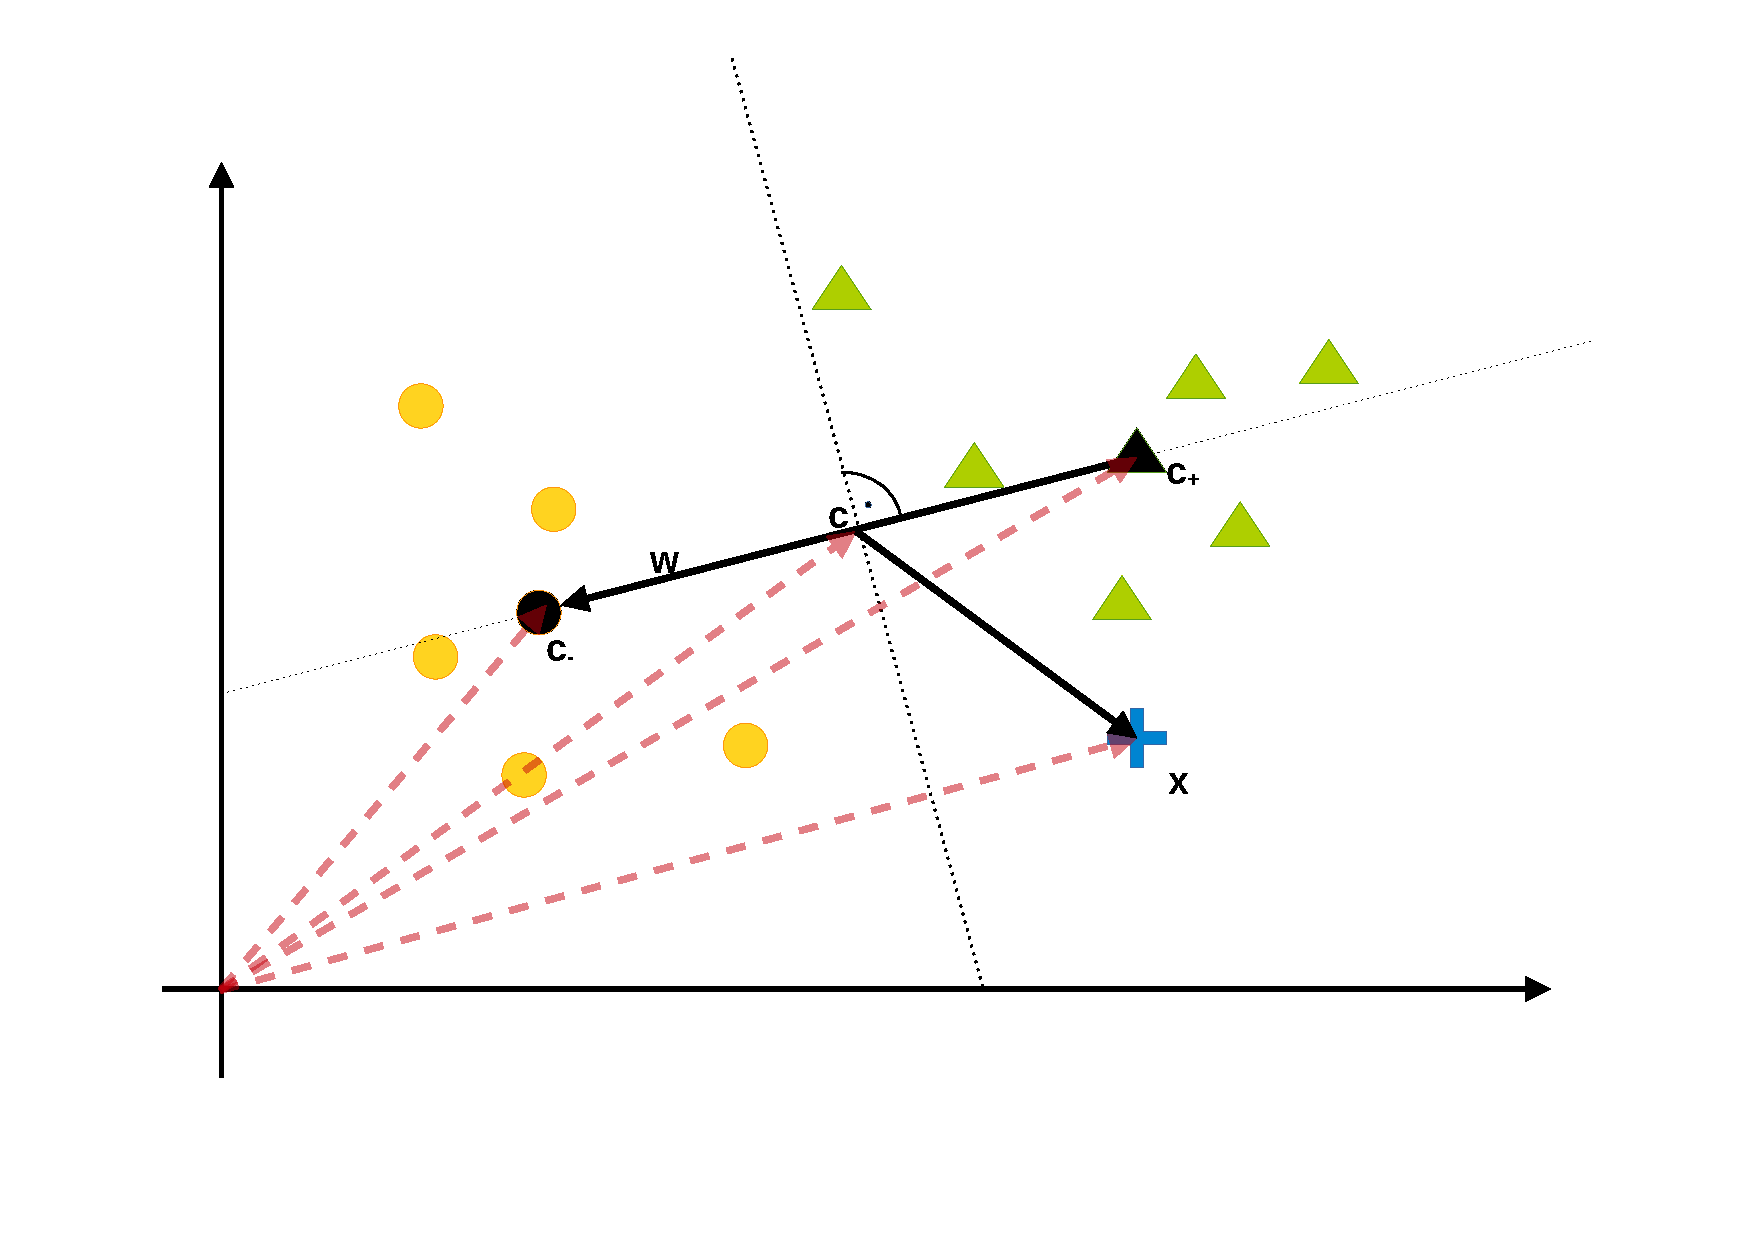
\includegraphics[width=0.3\textwidth]{images/svm1.pdf}
	\end{center}\pause
	$\mathbf{c}_+ = \frac{1}{n_+} \sum_{i\in\mathcal{I}_+} \mathbf{x}_i  \qquad \mathbf{c}_- = \frac{1}{n_-} \sum_{i\in\mathcal{I}_-} \mathbf{x}_i \qquad \mathbf{c} = \frac{\mathbf{c}_- + \mathbf{c}_+}{2} \qquad \mathbf{w} = \mathbf{c}_- - \mathbf{c}_+$\pause\vskip 0.3 cm
	
	$\mathbf{y} = \mathrm{sgn}\left\langle (\mathbf{x} - \mathbf{c}), \mathbf{w} \right\rangle \qquad \text{iloczyn skalarny} \left\langle \mathbf{a}, \mathbf{b}\right\rangle = \|\mathbf{a}\| \| \mathbf{b} \| \cos \theta$\pause\vskip 0.3 cm
	
	$\mathbf{y} = \mathrm{sgn}\left\langle (\mathbf{x} - \frac{\mathbf{c}_- + \mathbf{c}_+}{2}), \mathbf{c}_- - \mathbf{c}_+ \right\rangle = $\pause\vskip 0.3 cm
	
	$\mathbf{y} = \mathrm{sgn}( \left\langle \mathbf{x}, \mathbf{c}_- \right\rangle - \left\langle \mathbf{x}, \mathbf{c}_+ \right\rangle  
	\underbrace{-\left\langle \frac{\mathbf{c}_- + \mathbf{c}_+}{2} , \mathbf{c}_-\right\rangle + \left\langle \frac{\mathbf{c}_- + \mathbf{c}_+}{2}, \mathbf{c}_+\right\rangle}_{\quad\text{nie zależy od}\: \mathbf{x}} )$ 
\end{frame}
\begin{frame}
	\begin{center}
		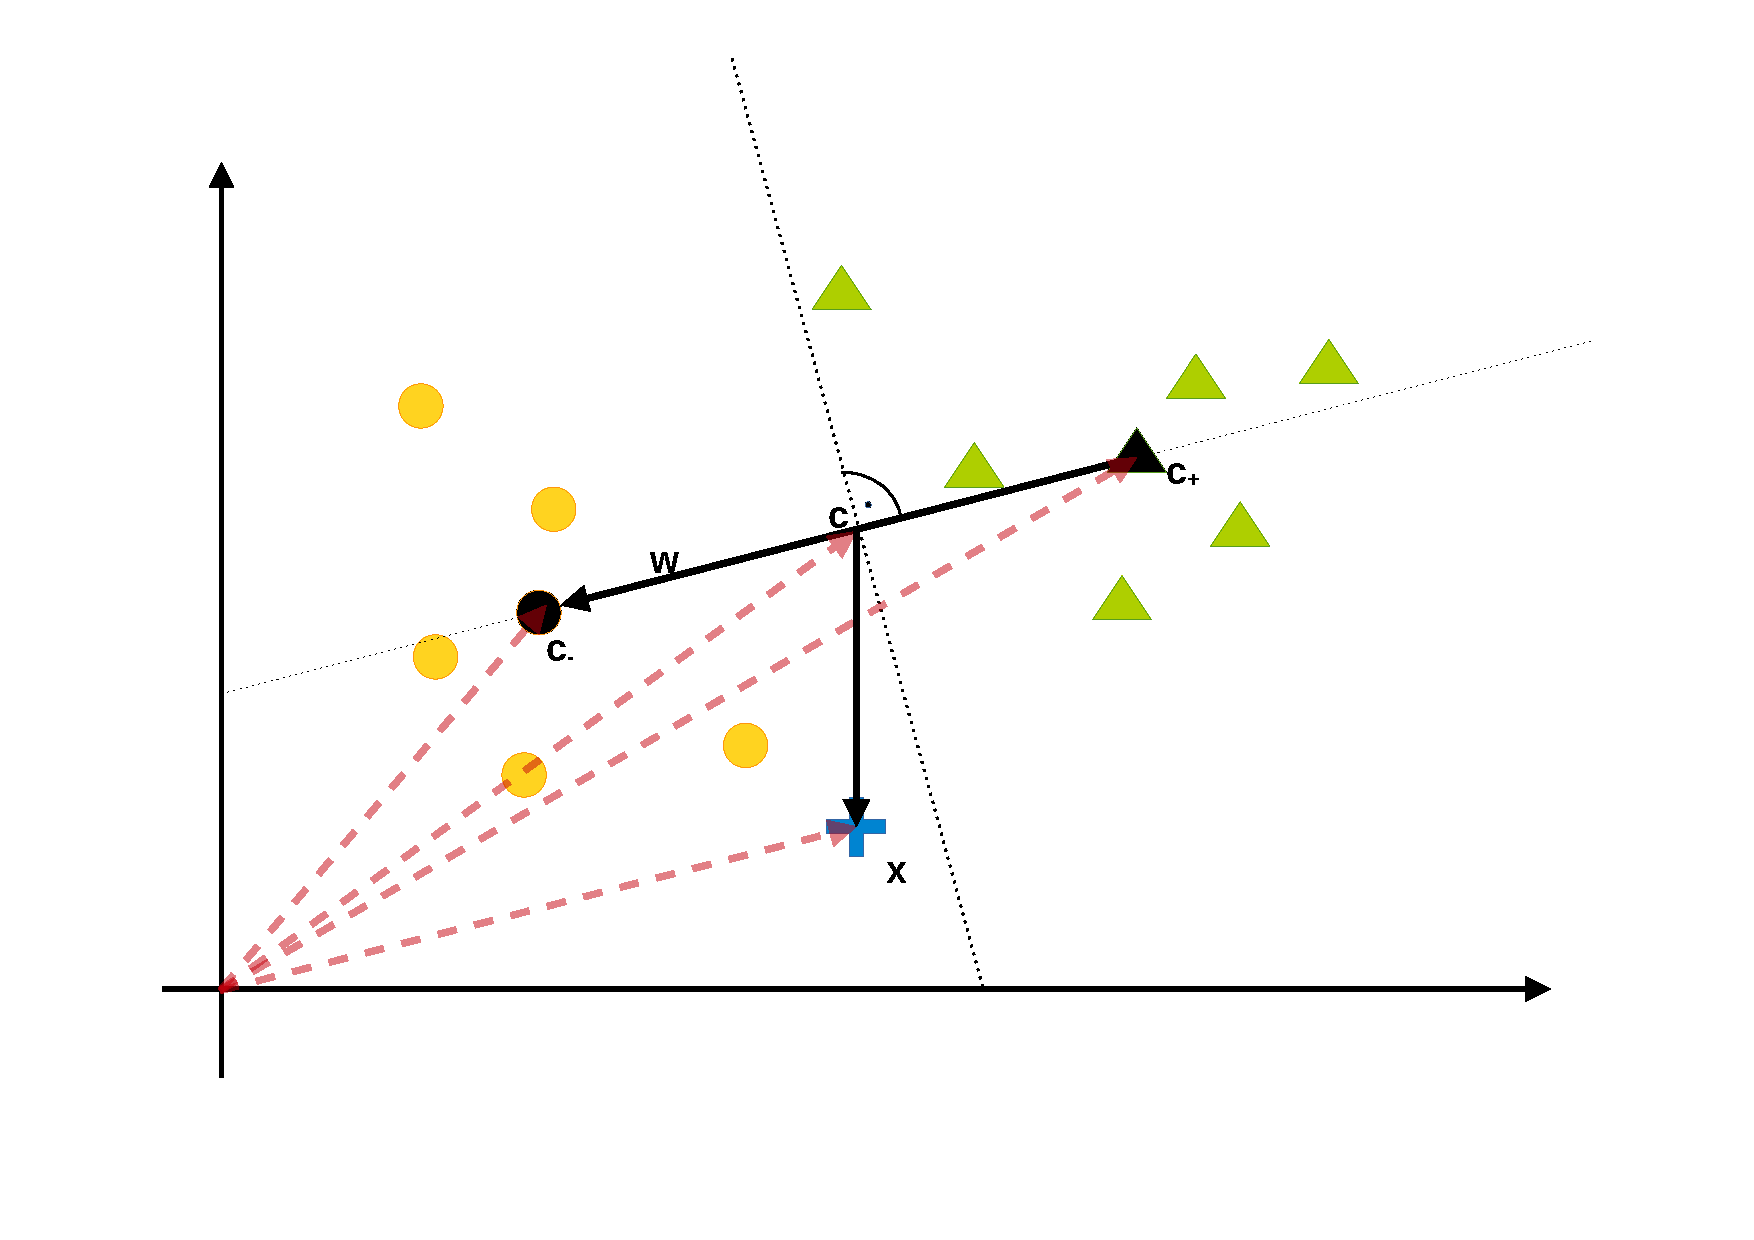
\includegraphics[width=0.3\textwidth]{images/svma.pdf}
		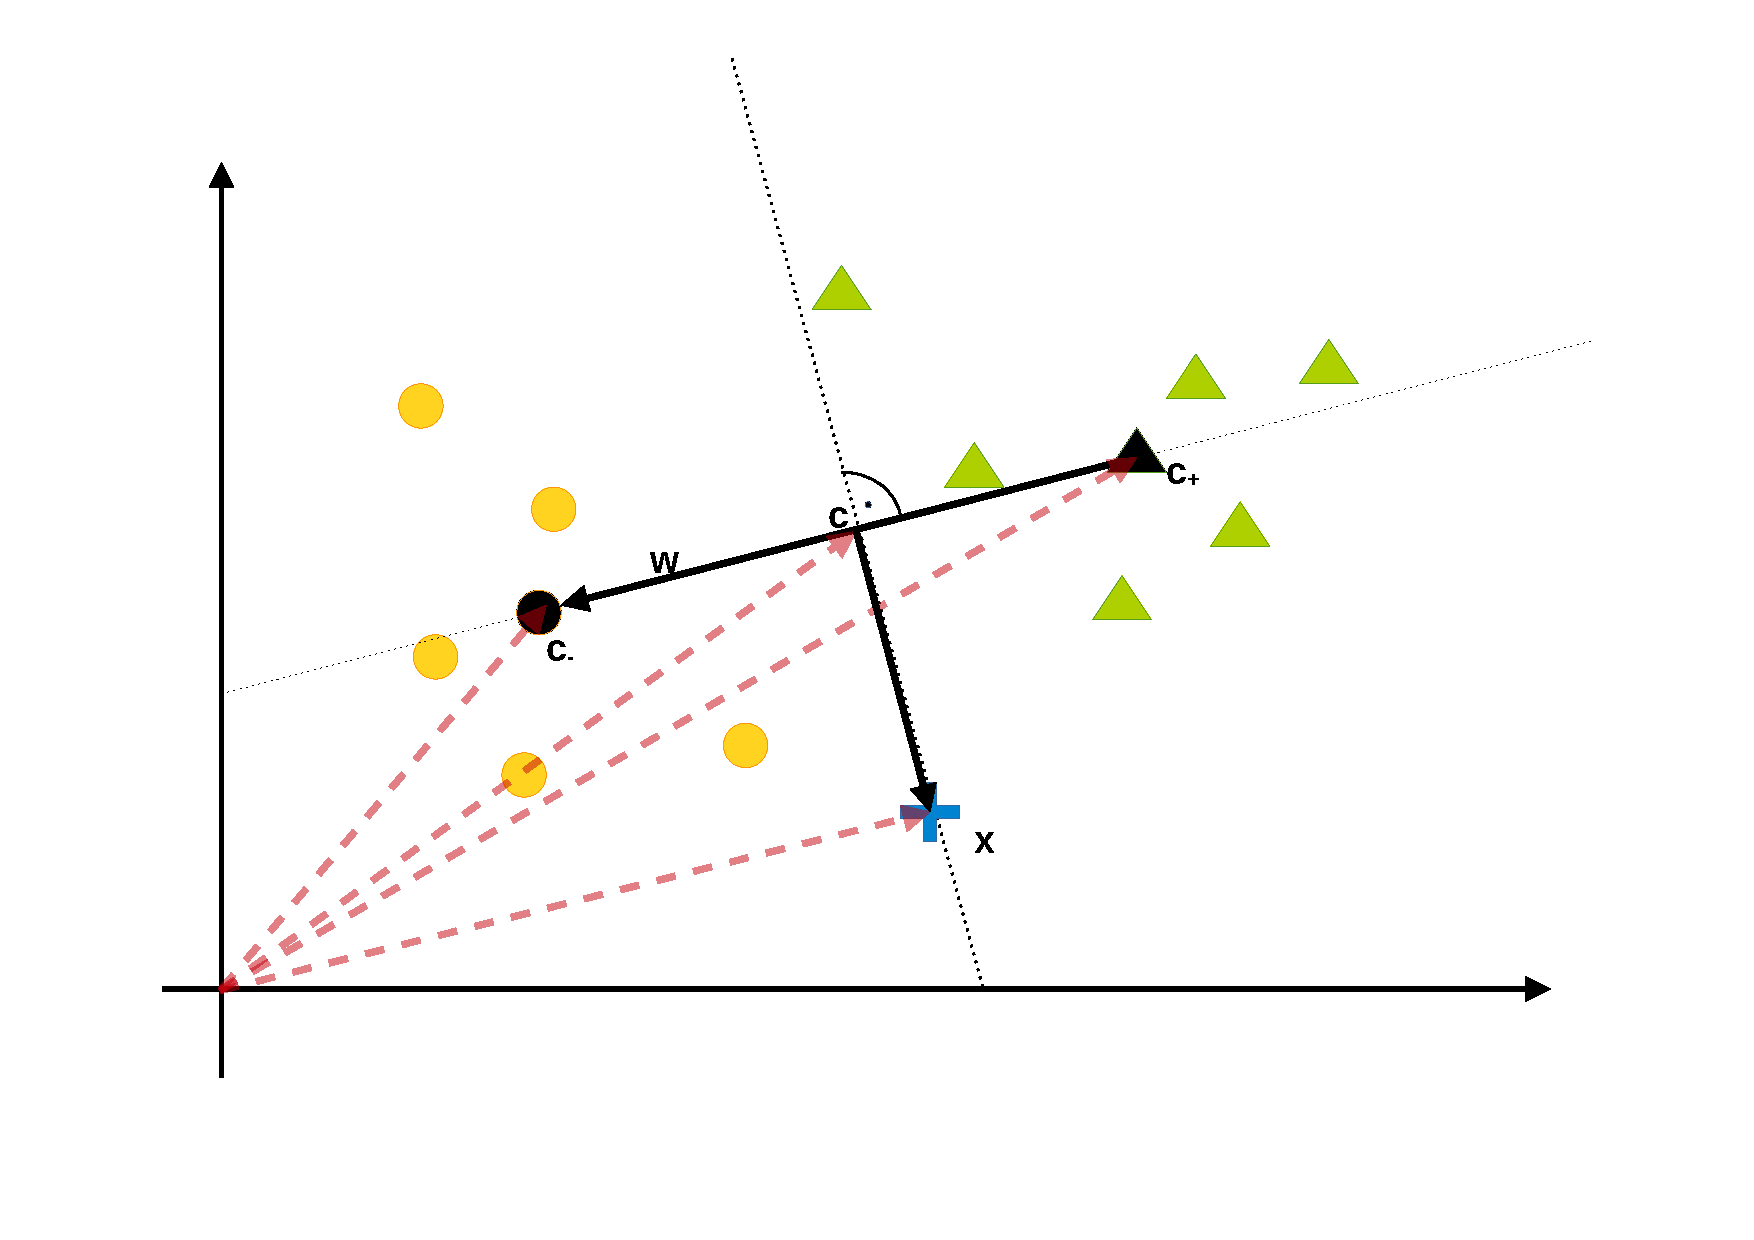
\includegraphics[width=0.3\textwidth]{images/svm0.pdf}
		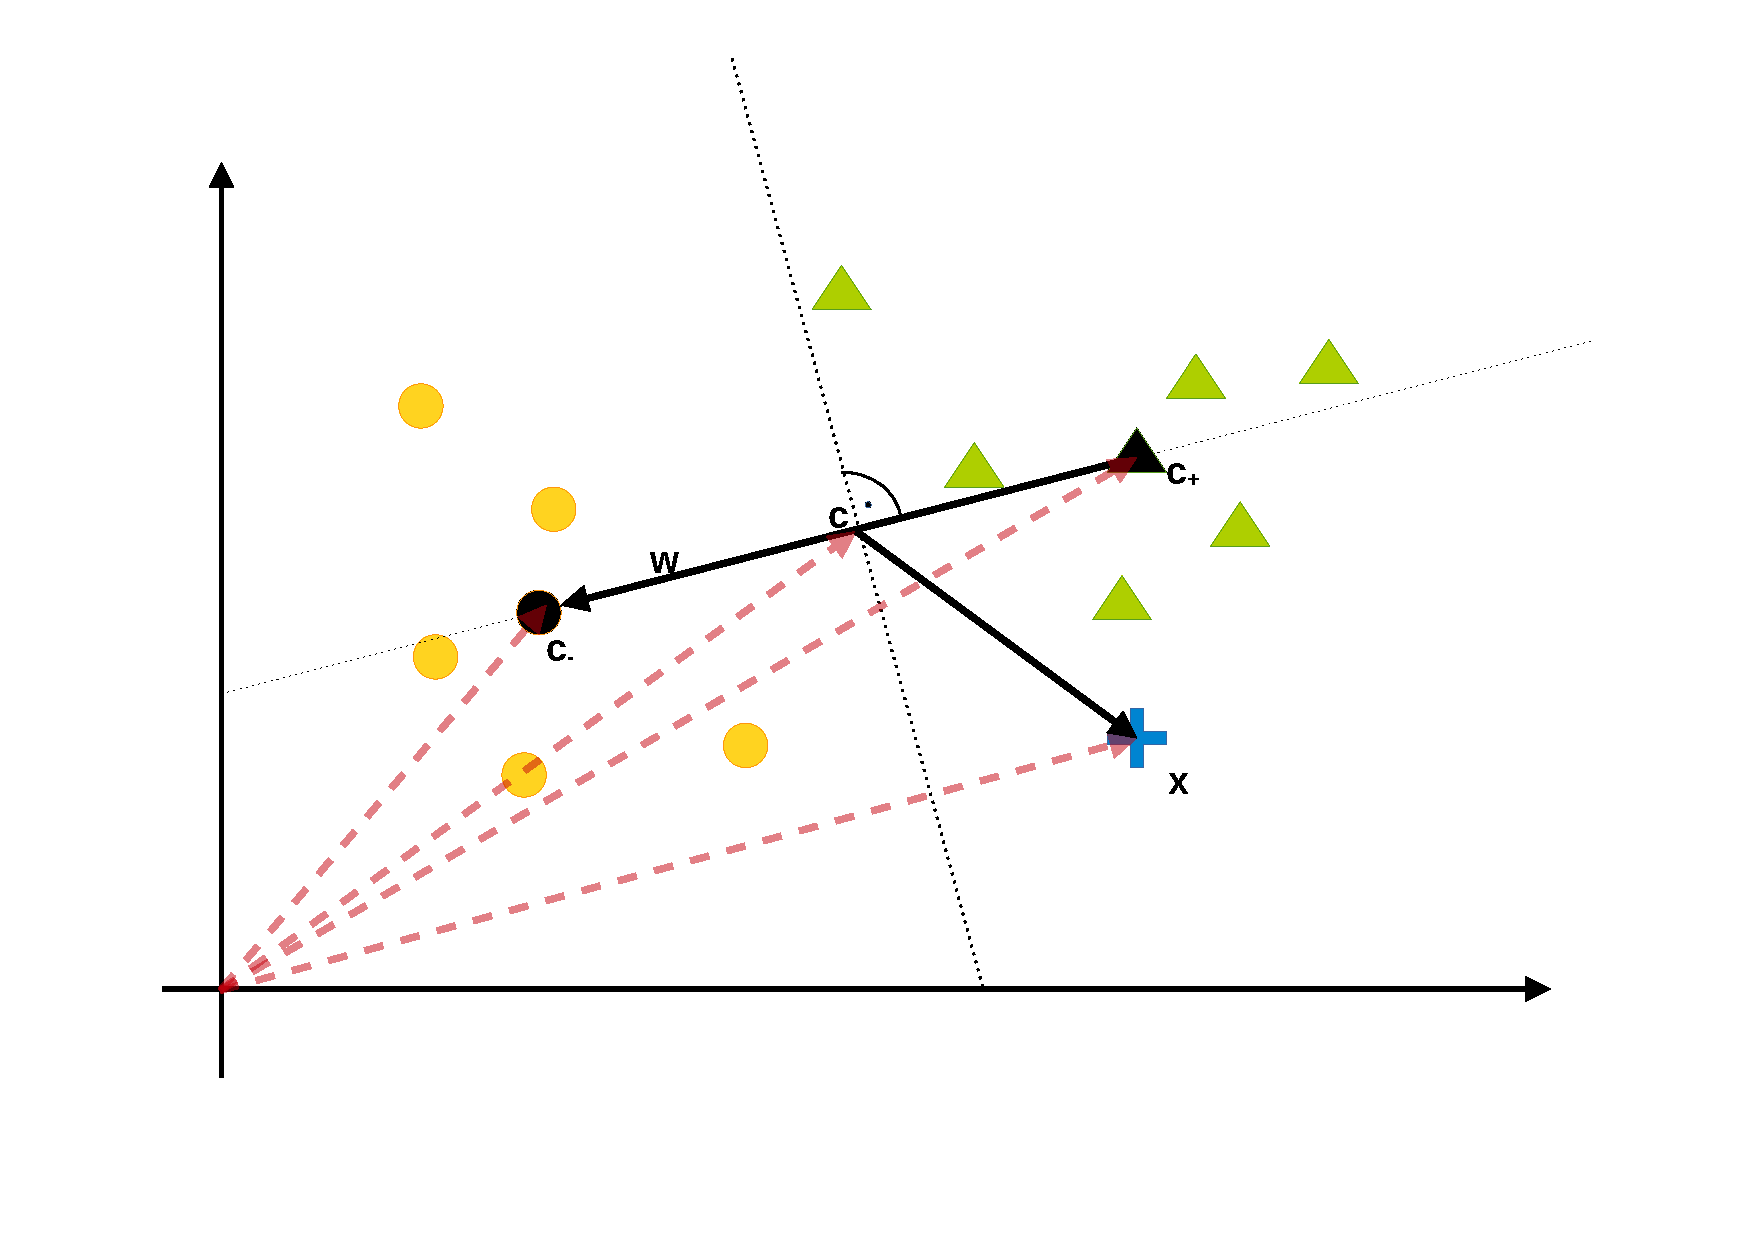
\includegraphics[width=0.3\textwidth]{images/svm1.pdf}
	\end{center}
	$\mathbf{y} = \mathrm{sgn}( \left\langle \mathbf{x}, \mathbf{c}_- \right\rangle - \left\langle \mathbf{x}, \mathbf{c}_+ \right\rangle + b) \qquad \mathbf{c}_- = \frac{1}{n_-} \sum_{i\in\mathcal{I}_-} \mathbf{x}_i$ \pause\vskip 0.3 cm
	
	$\mathbf{y} = \mathrm{sgn}\left( \frac{1}{n_-} \sum_{i\in\mathcal{I}_-} \left\langle \mathbf{x}_i, \mathbf{x} \right\rangle 
	- \frac{1}{n_+} \sum_{i\in\mathcal{I}_+} \left\langle \mathbf{x}_i, \mathbf{x} \right\rangle + b\right)$ \pause\vskip 0.3 cm
	
	$\mathbf{y} = \mathrm{sgn}\left( -\sum_i y_i\left\langle \mathbf{x}_i, \mathbf{x} \right\rangle + b\right)$ \pause\vskip 0.3 cm
	
	$\mathbf{y} = \mathrm{sgn}\left(\sum_i \alpha_i\left\langle \mathbf{x}_i, \mathbf{x} \right\rangle + b\right)$
\end{frame}

\begin{frame}{Margines}\begin{center}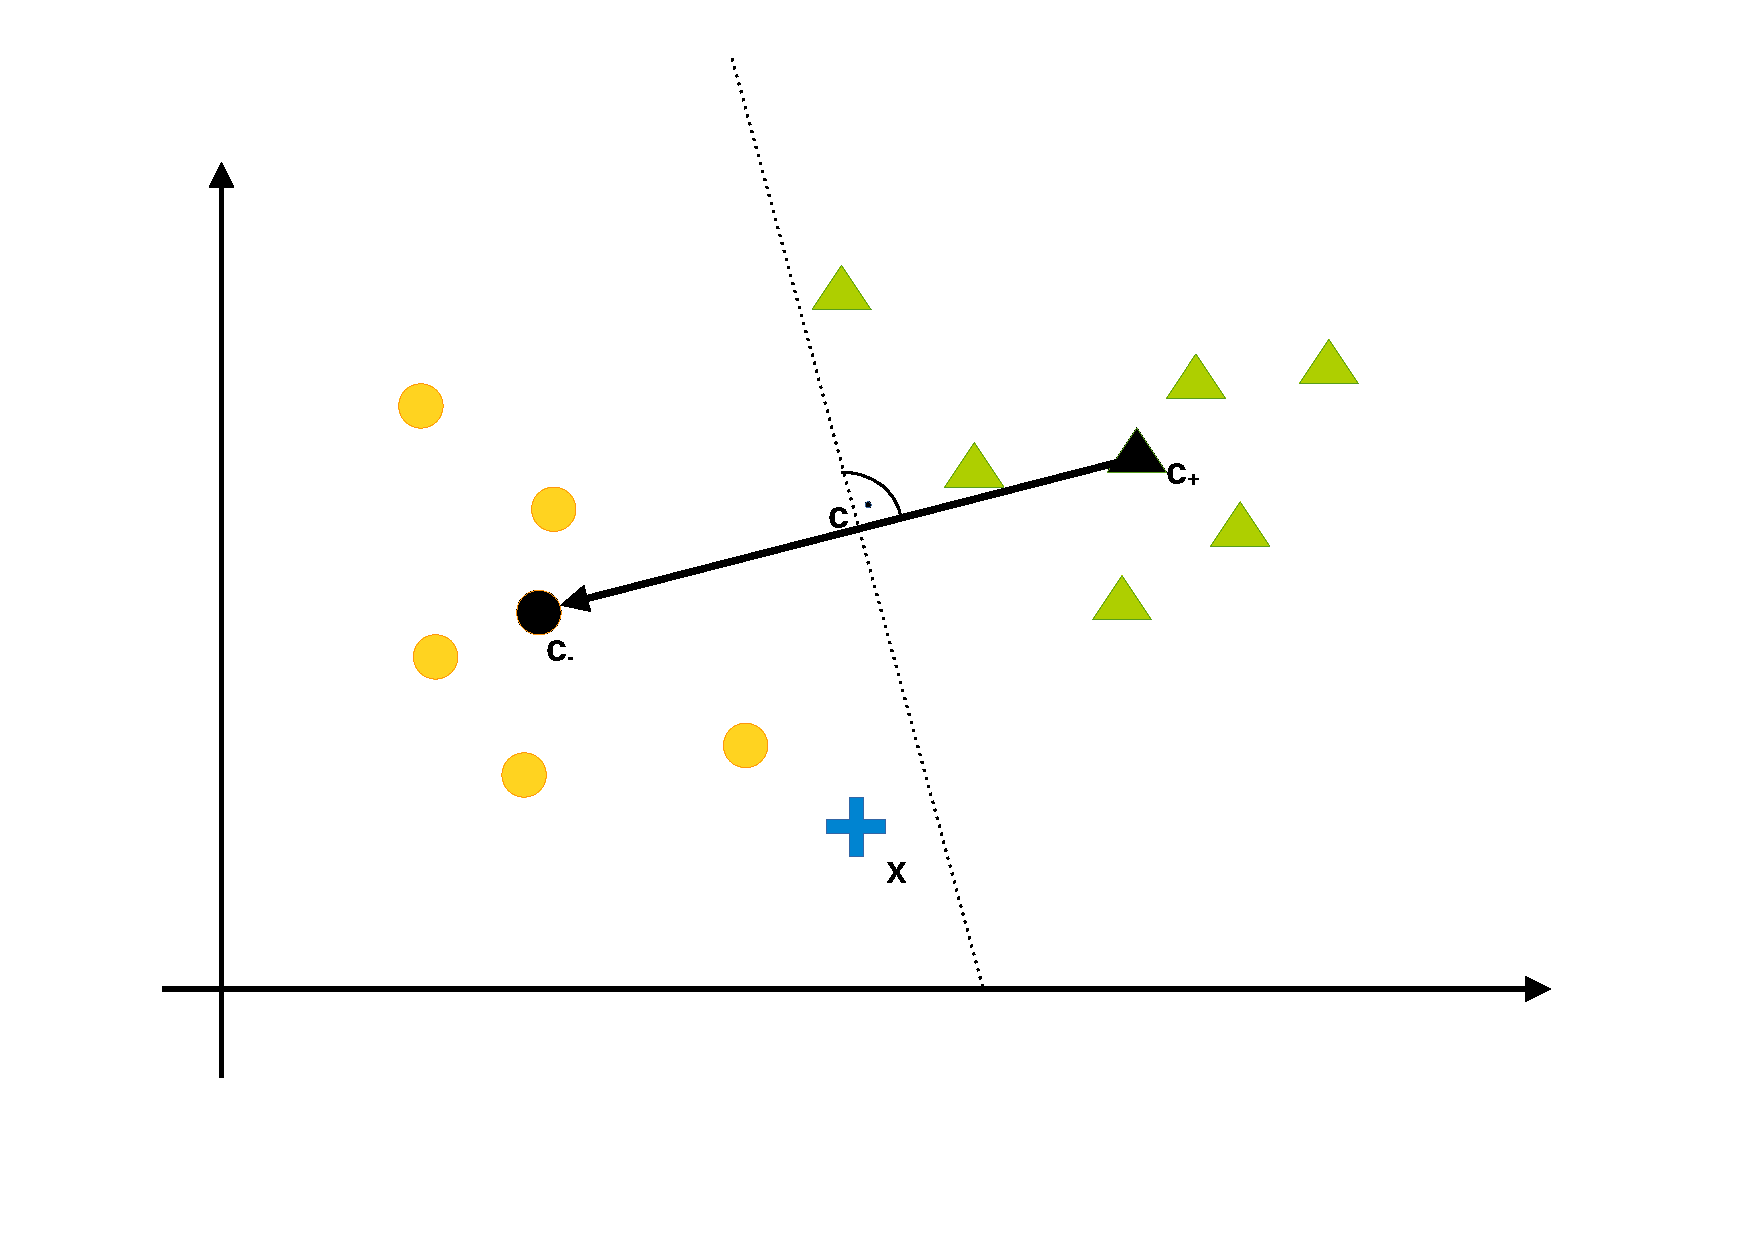
\includegraphics[width=0.7\textwidth]{images/svmm.pdf}\end{center}\end{frame}
\begin{frame}{Margines}\begin{center}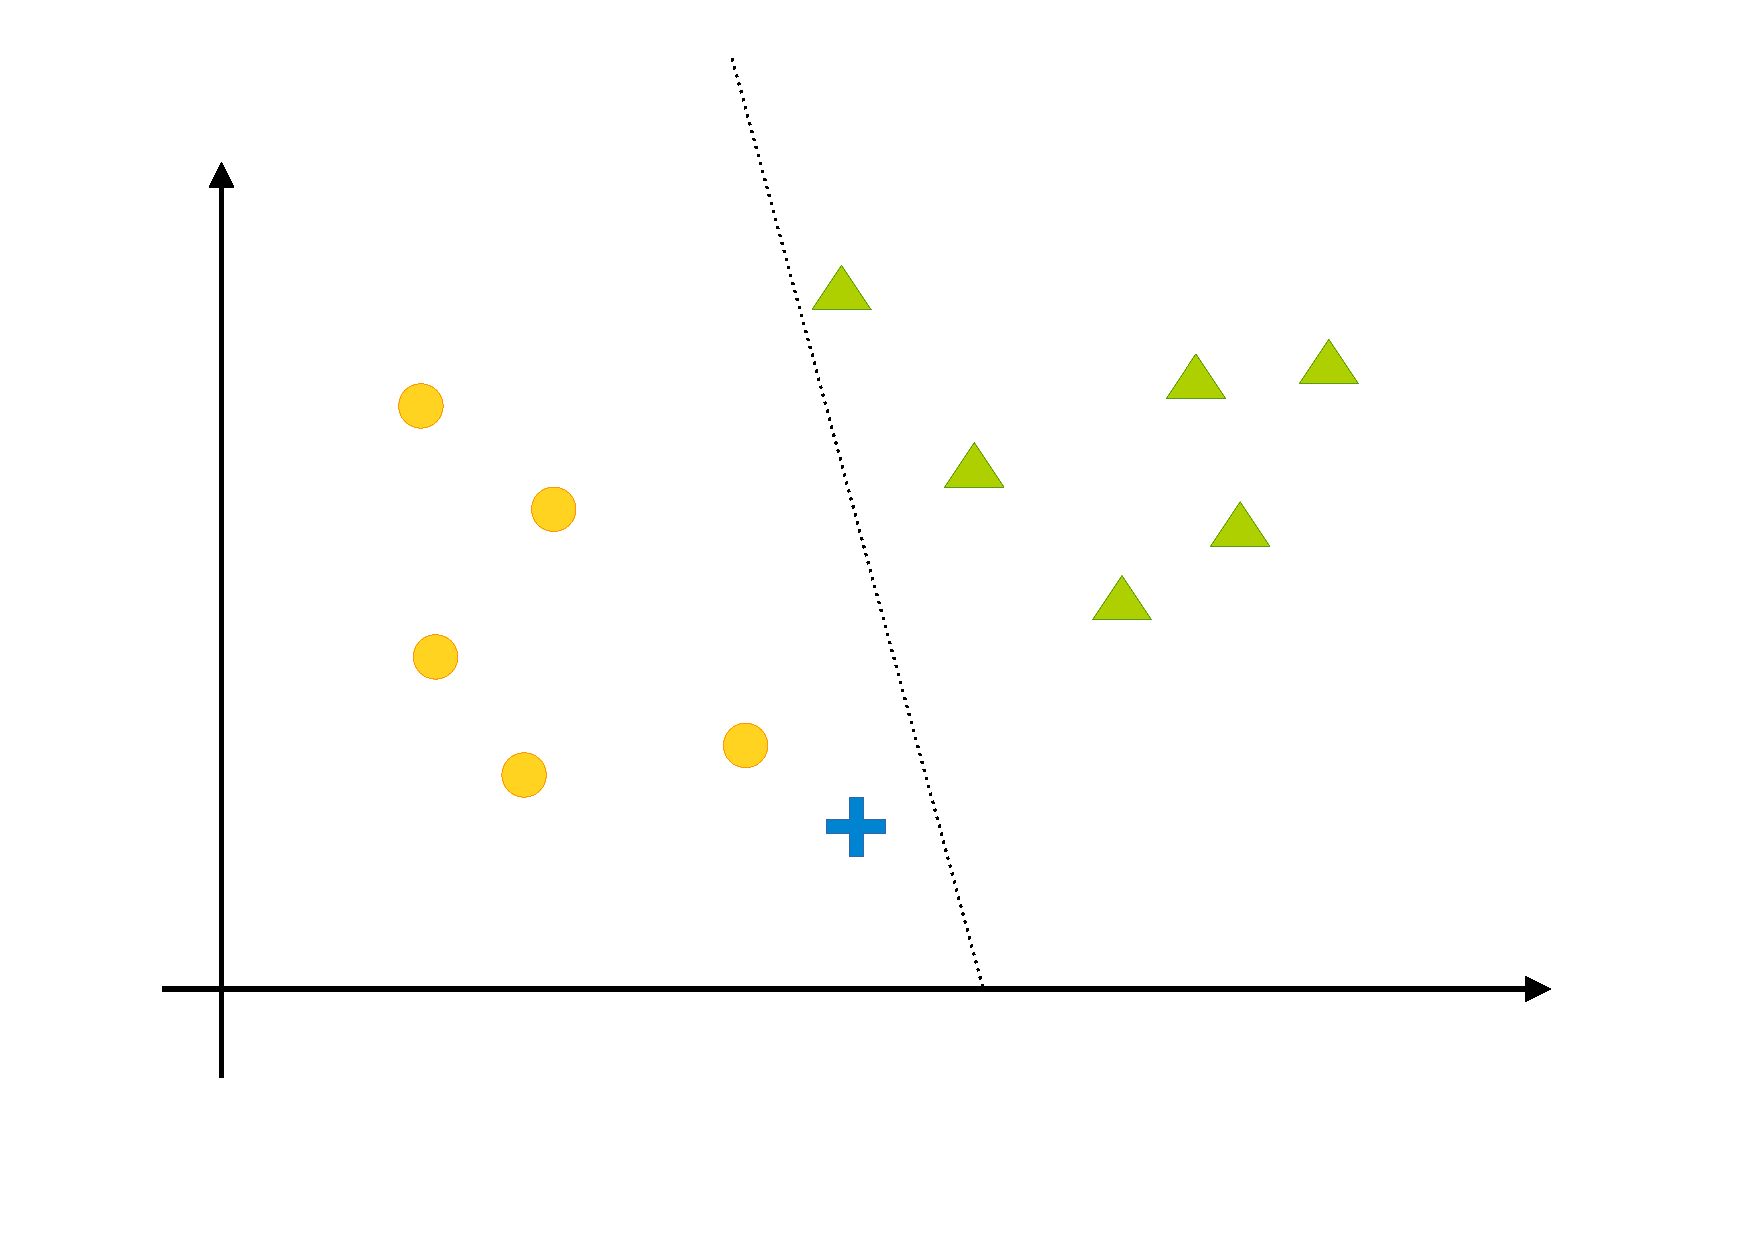
\includegraphics[width=0.7\textwidth]{images/svmm1.pdf}\end{center}\end{frame}
\begin{frame}{Margines}\begin{center}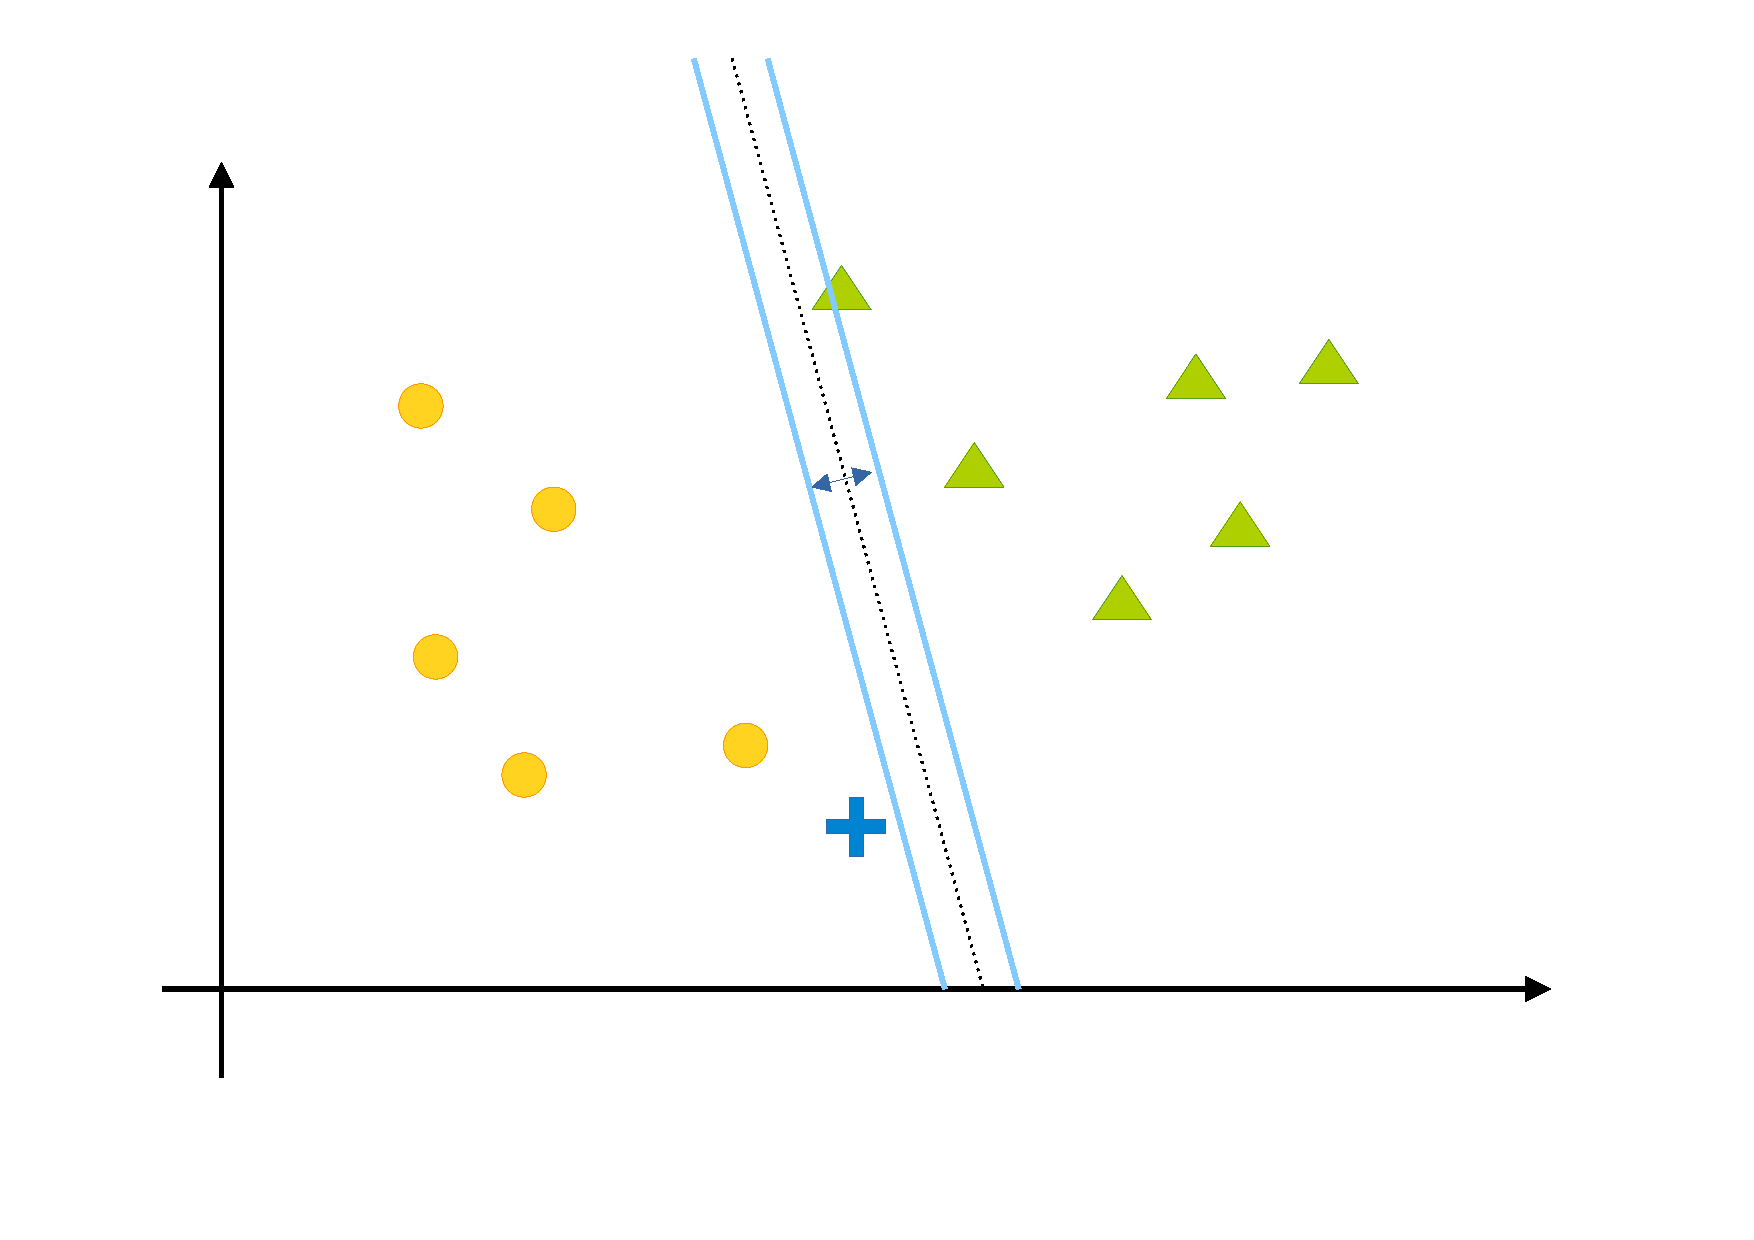
\includegraphics[width=0.7\textwidth]{images/svmm2.pdf}\end{center}\end{frame}
\begin{frame}{Margines}\begin{center}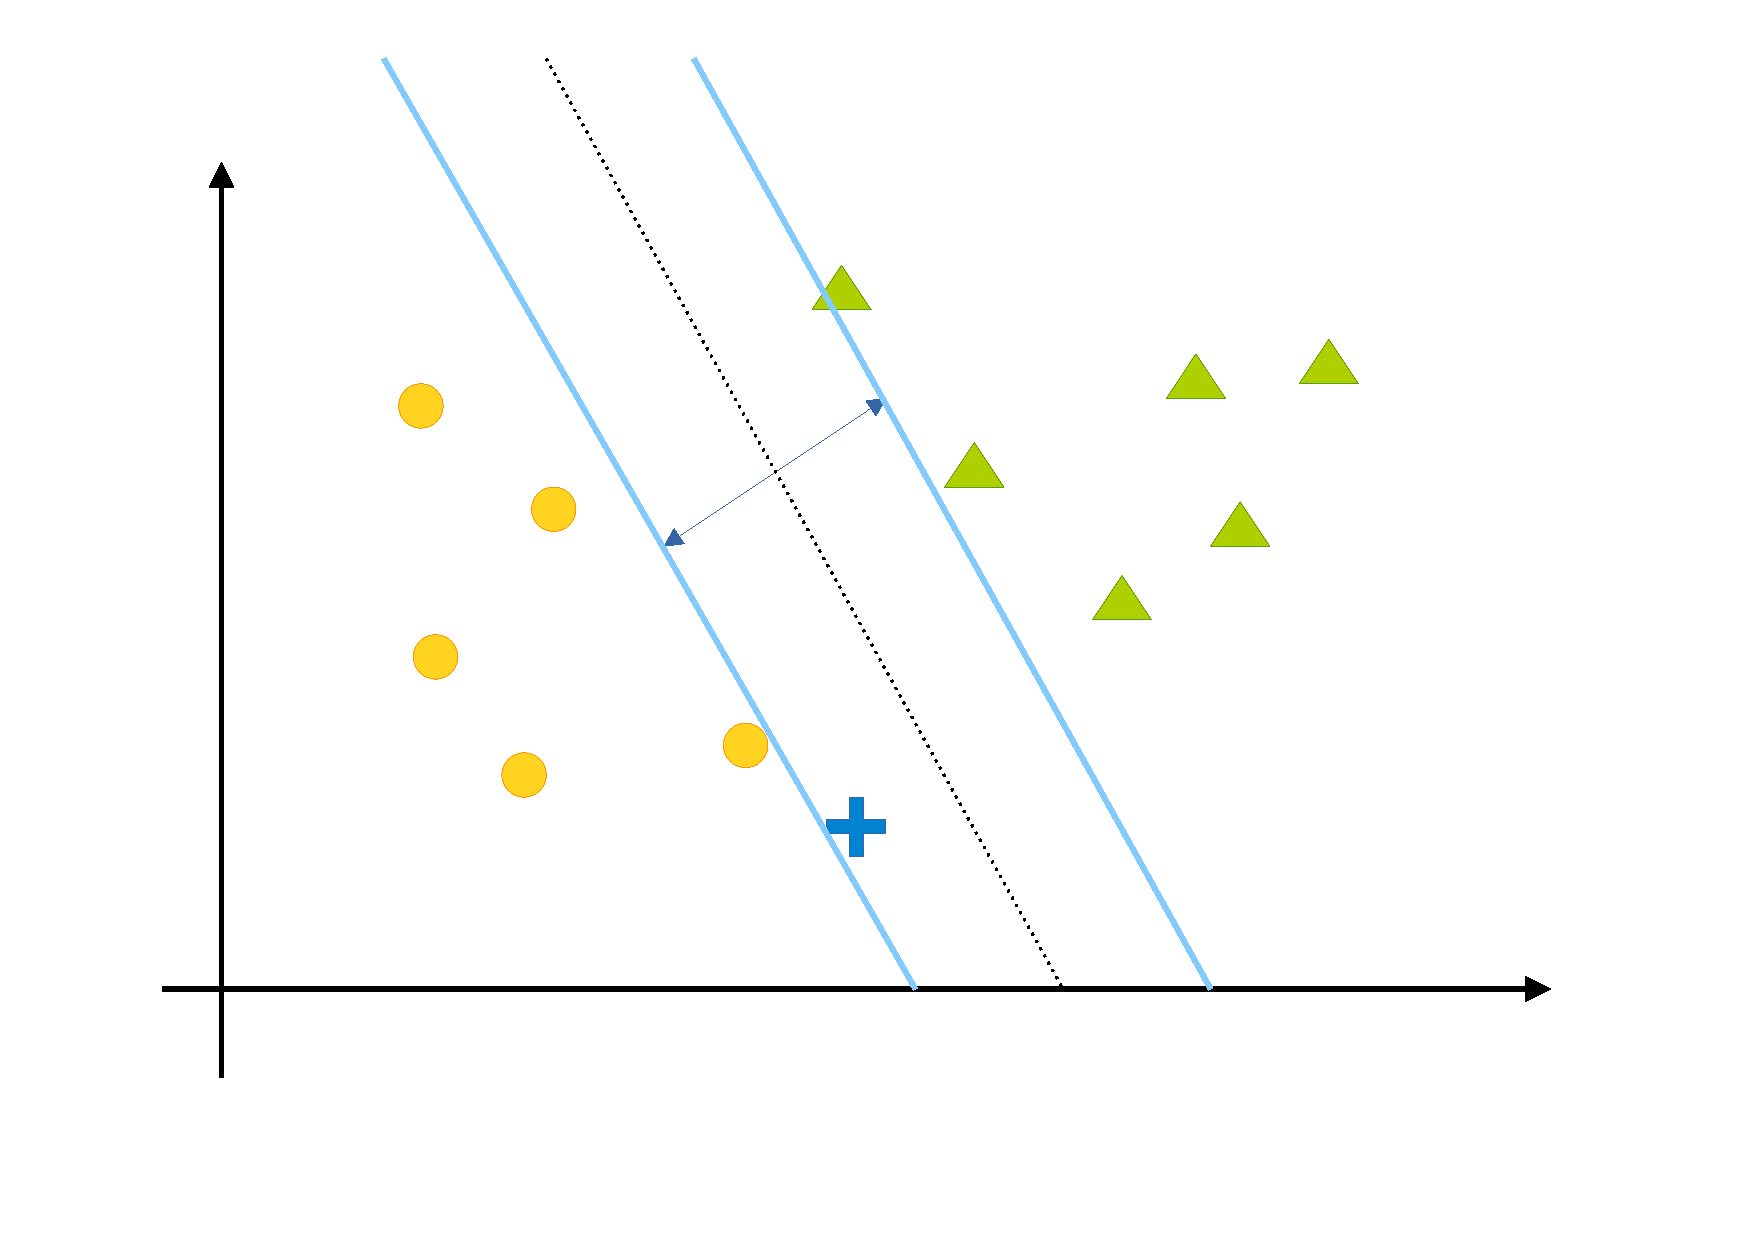
\includegraphics[width=0.7\textwidth]{images/svmm3.pdf}\end{center}\end{frame}

\begin{frame}{SVM}
	\begin{center}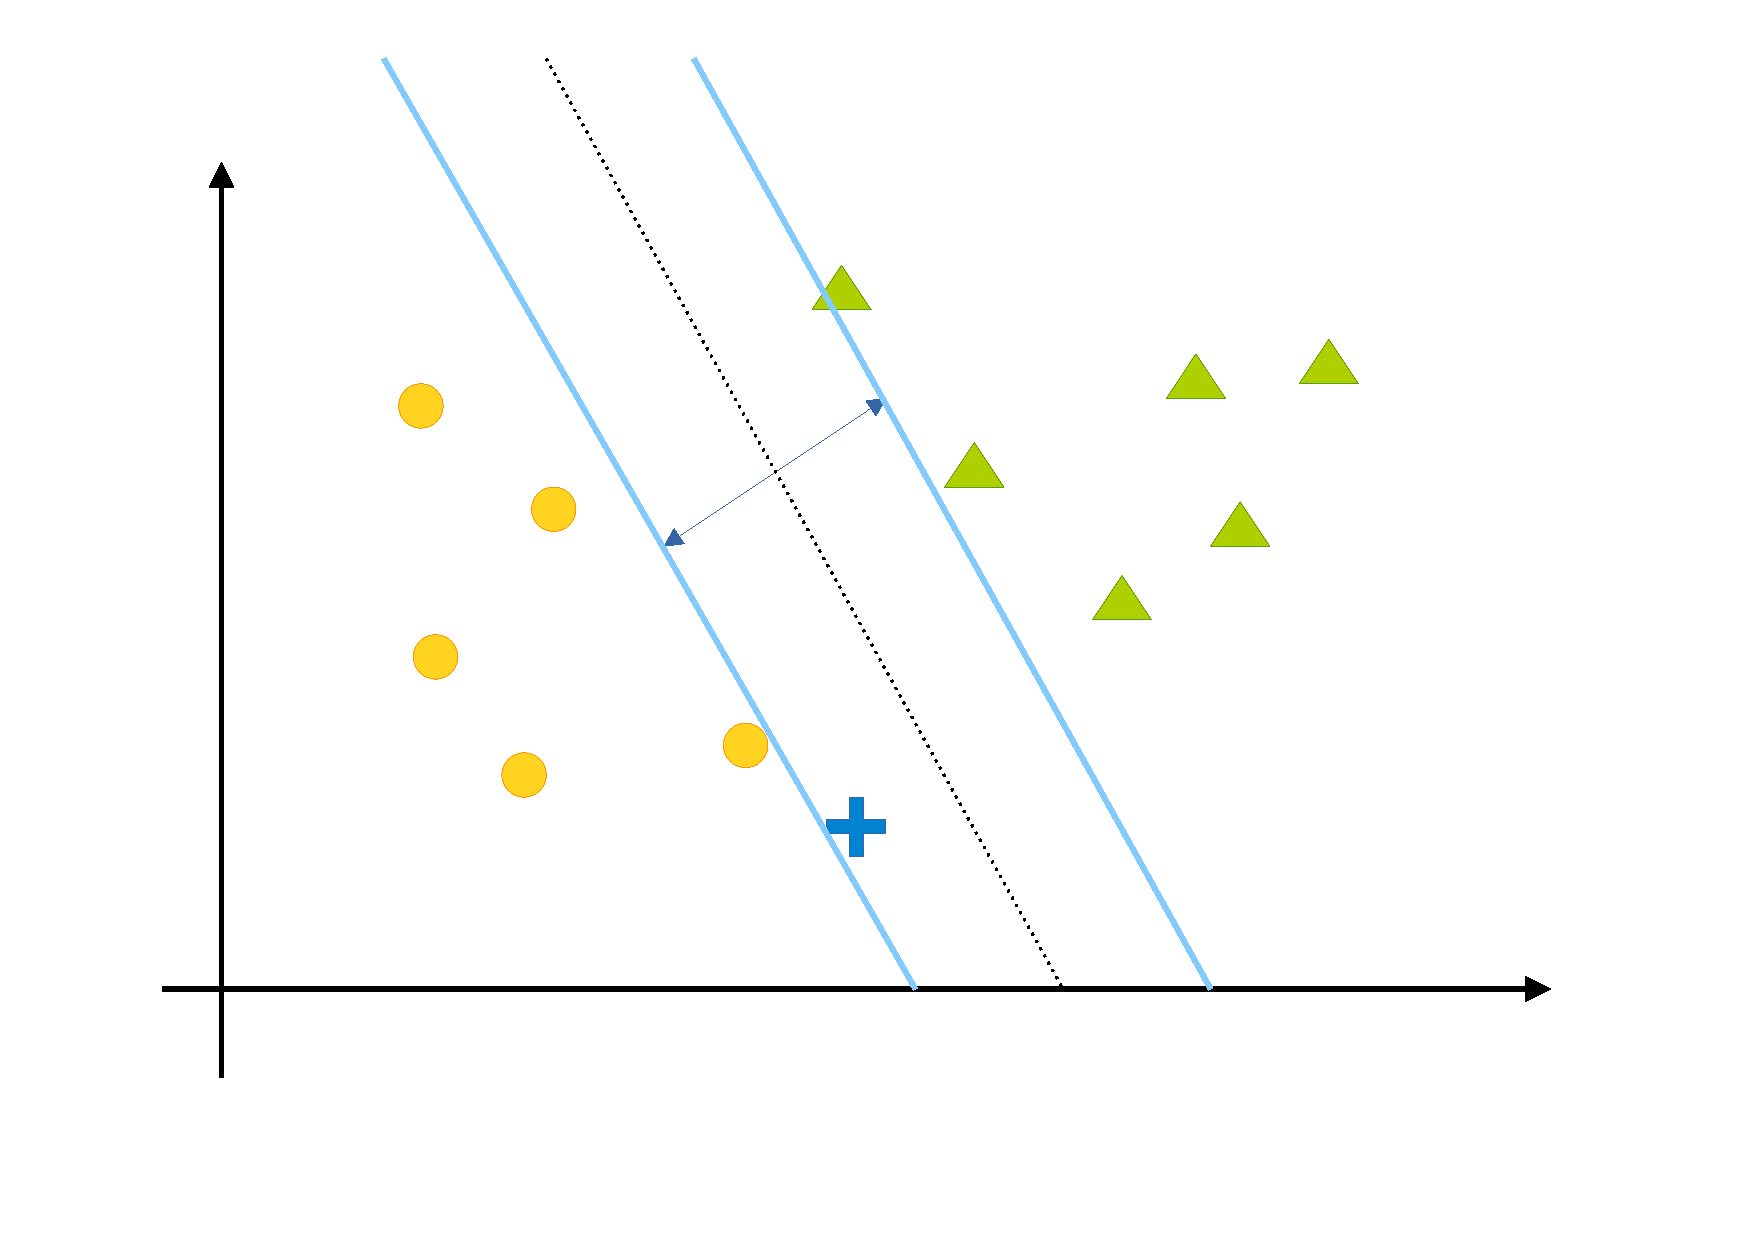
\includegraphics[width=0.25\textwidth]{images/svmm3.pdf}\end{center}
	
	$\mathbf{y} = \mathrm{sgn}\left(\sum_i \alpha_i\left\langle \mathbf{x}_i, \mathbf{x} \right\rangle + b\right)$\vskip 0.3 cm
	
	$\underset{\boldsymbol{\alpha}\in\mathbb{R}^n}{\mathrm{maximize}} W(\boldsymbol{\alpha}) = \sum_i \alpha_i - \frac{1}{2} \sum_{ij} \alpha_i \alpha_j y_i y_j \left\langle \mathbf{x}_i, \mathbf{x}_j \right\rangle$\vskip 0.3 cm
	ograniczenia $\alpha_i \geq 0, \sum_i \alpha_i y_i = 0$
\end{frame}
\begin{frame}{SVM}
	\begin{center}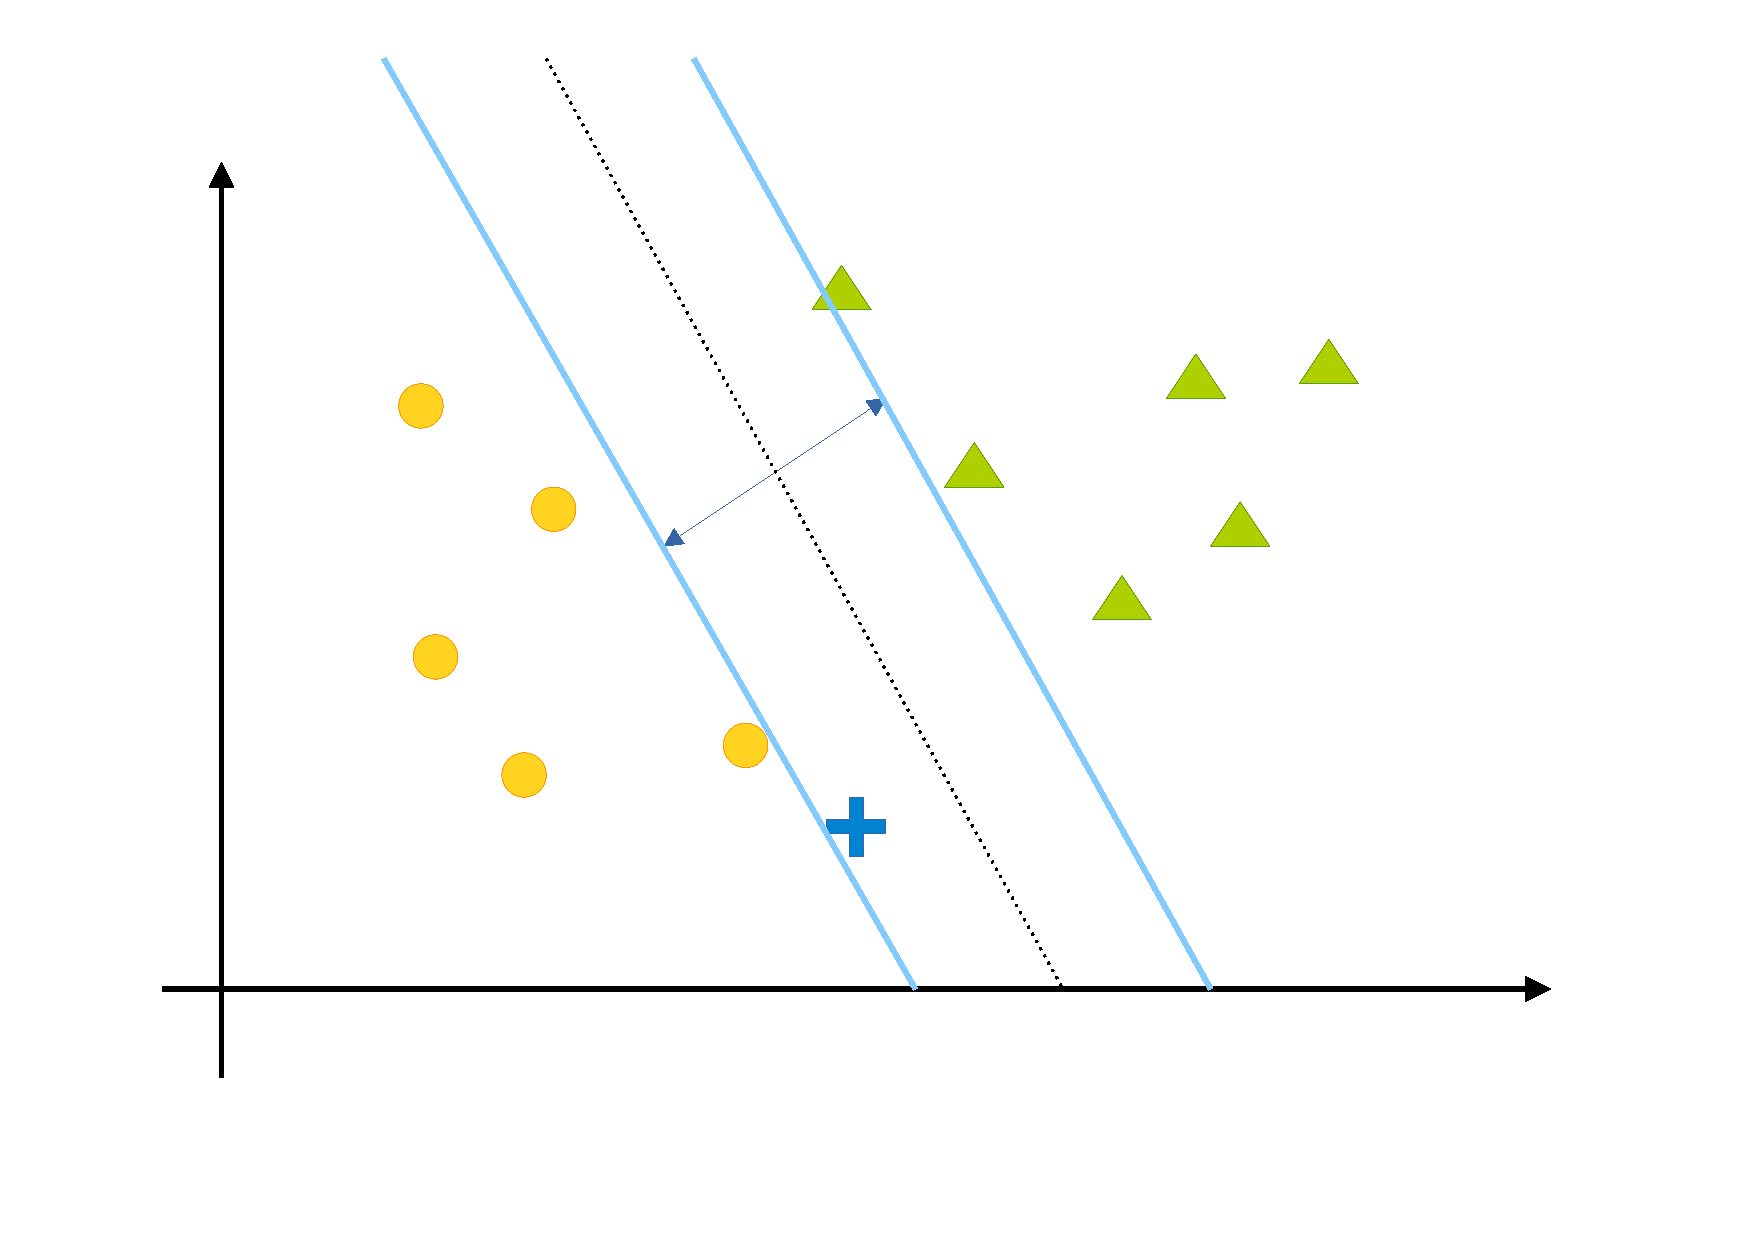
\includegraphics[width=0.25\textwidth]{images/svmm3.pdf}\end{center}
	
	$\mathbf{y} = \mathrm{sgn}\left(\sum_i \alpha_i\left\langle \mathbf{x}_i, \mathbf{x} \right\rangle + b\right)$\vskip 0.3 cm\pause
	
	\begin{description}
		\item[zalety] 	Brak [hiper]parametrów!\\
		(Parametry $\alpha_i$ z optymalizacji, ale nie potrzeba np. learning rate, rozmiaru warstw, \dots)\pause
		\item[wady] Tylko dla separowalnych zbiorów danych, których klasy da się rozdzielić hiperpłaszczyzną
	\end{description}
\end{frame}

\begin{frame}\begin{center}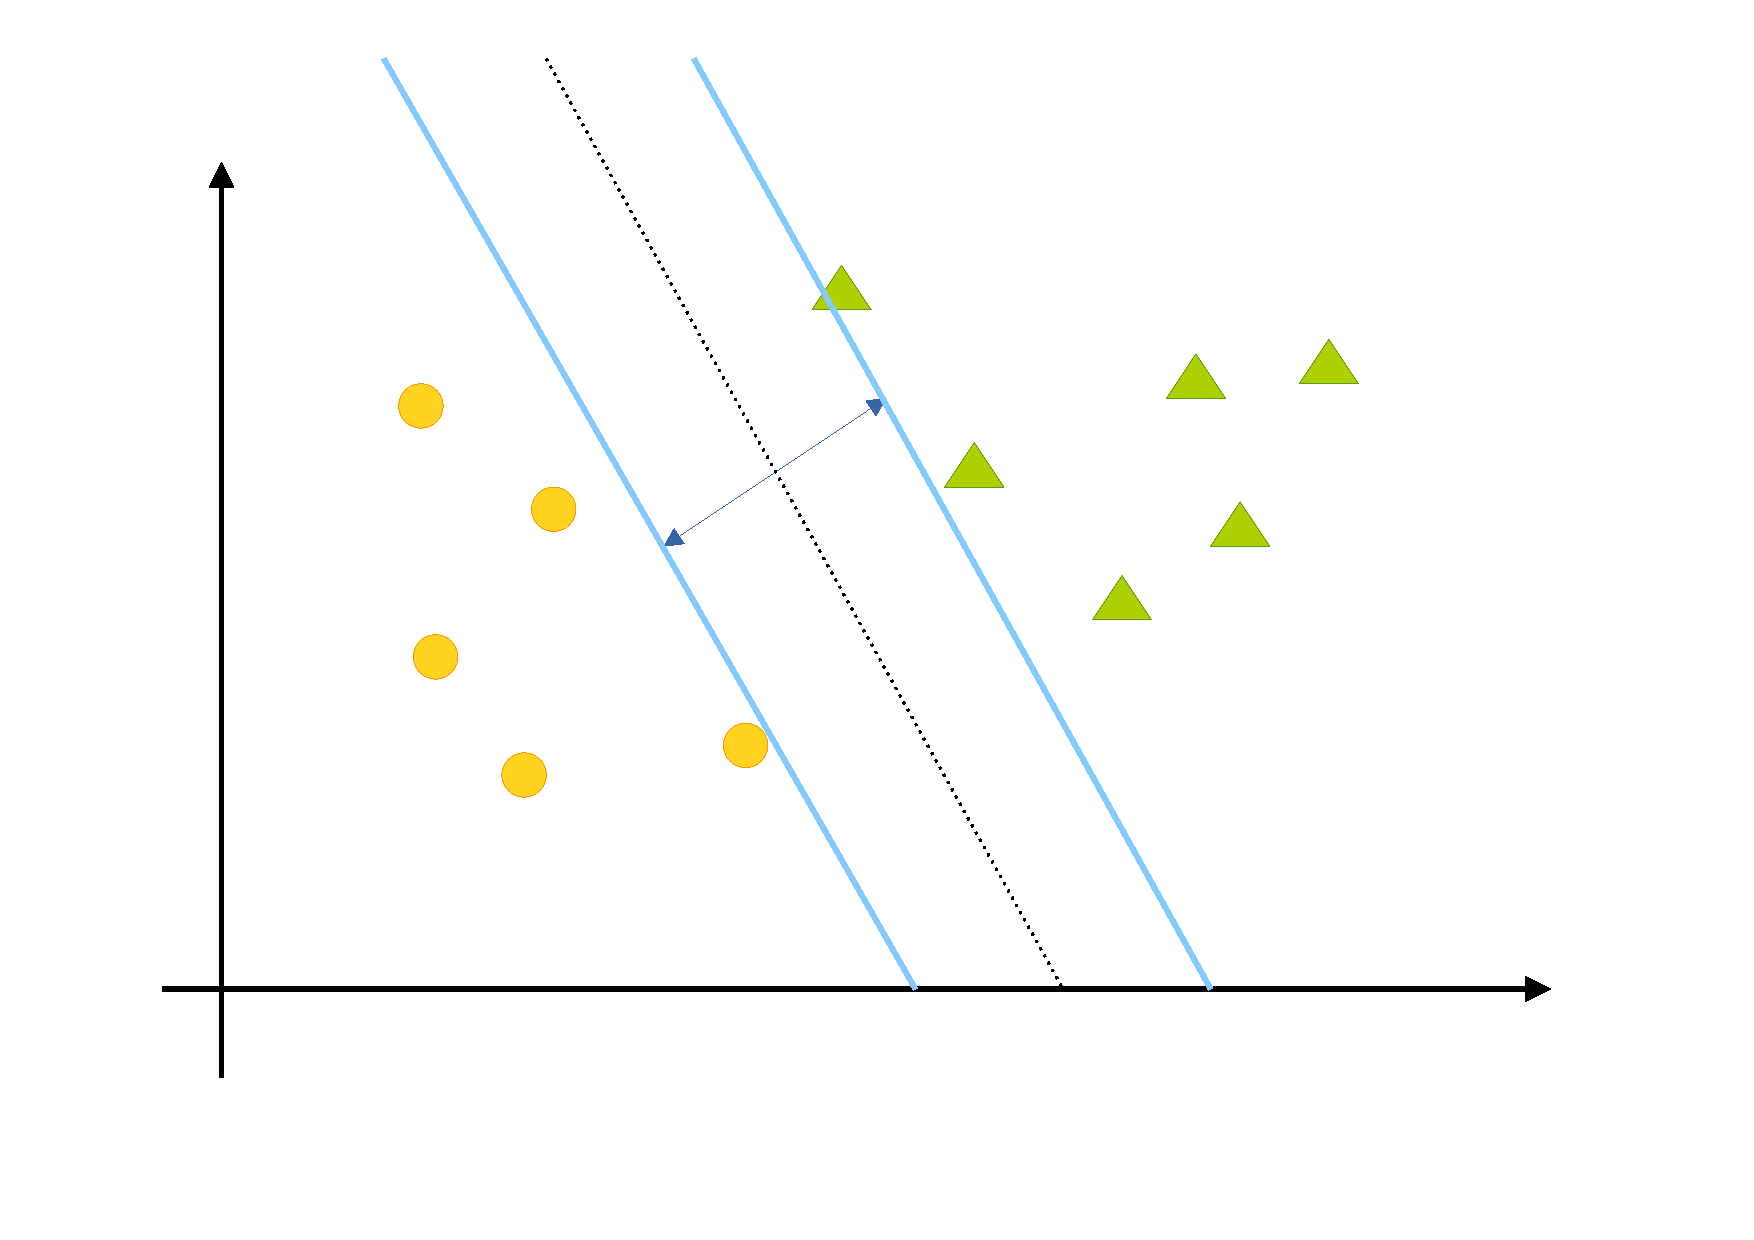
\includegraphics[width=0.7\textwidth]{images/svmm_c.pdf}\end{center}\end{frame}
\begin{frame}\begin{center}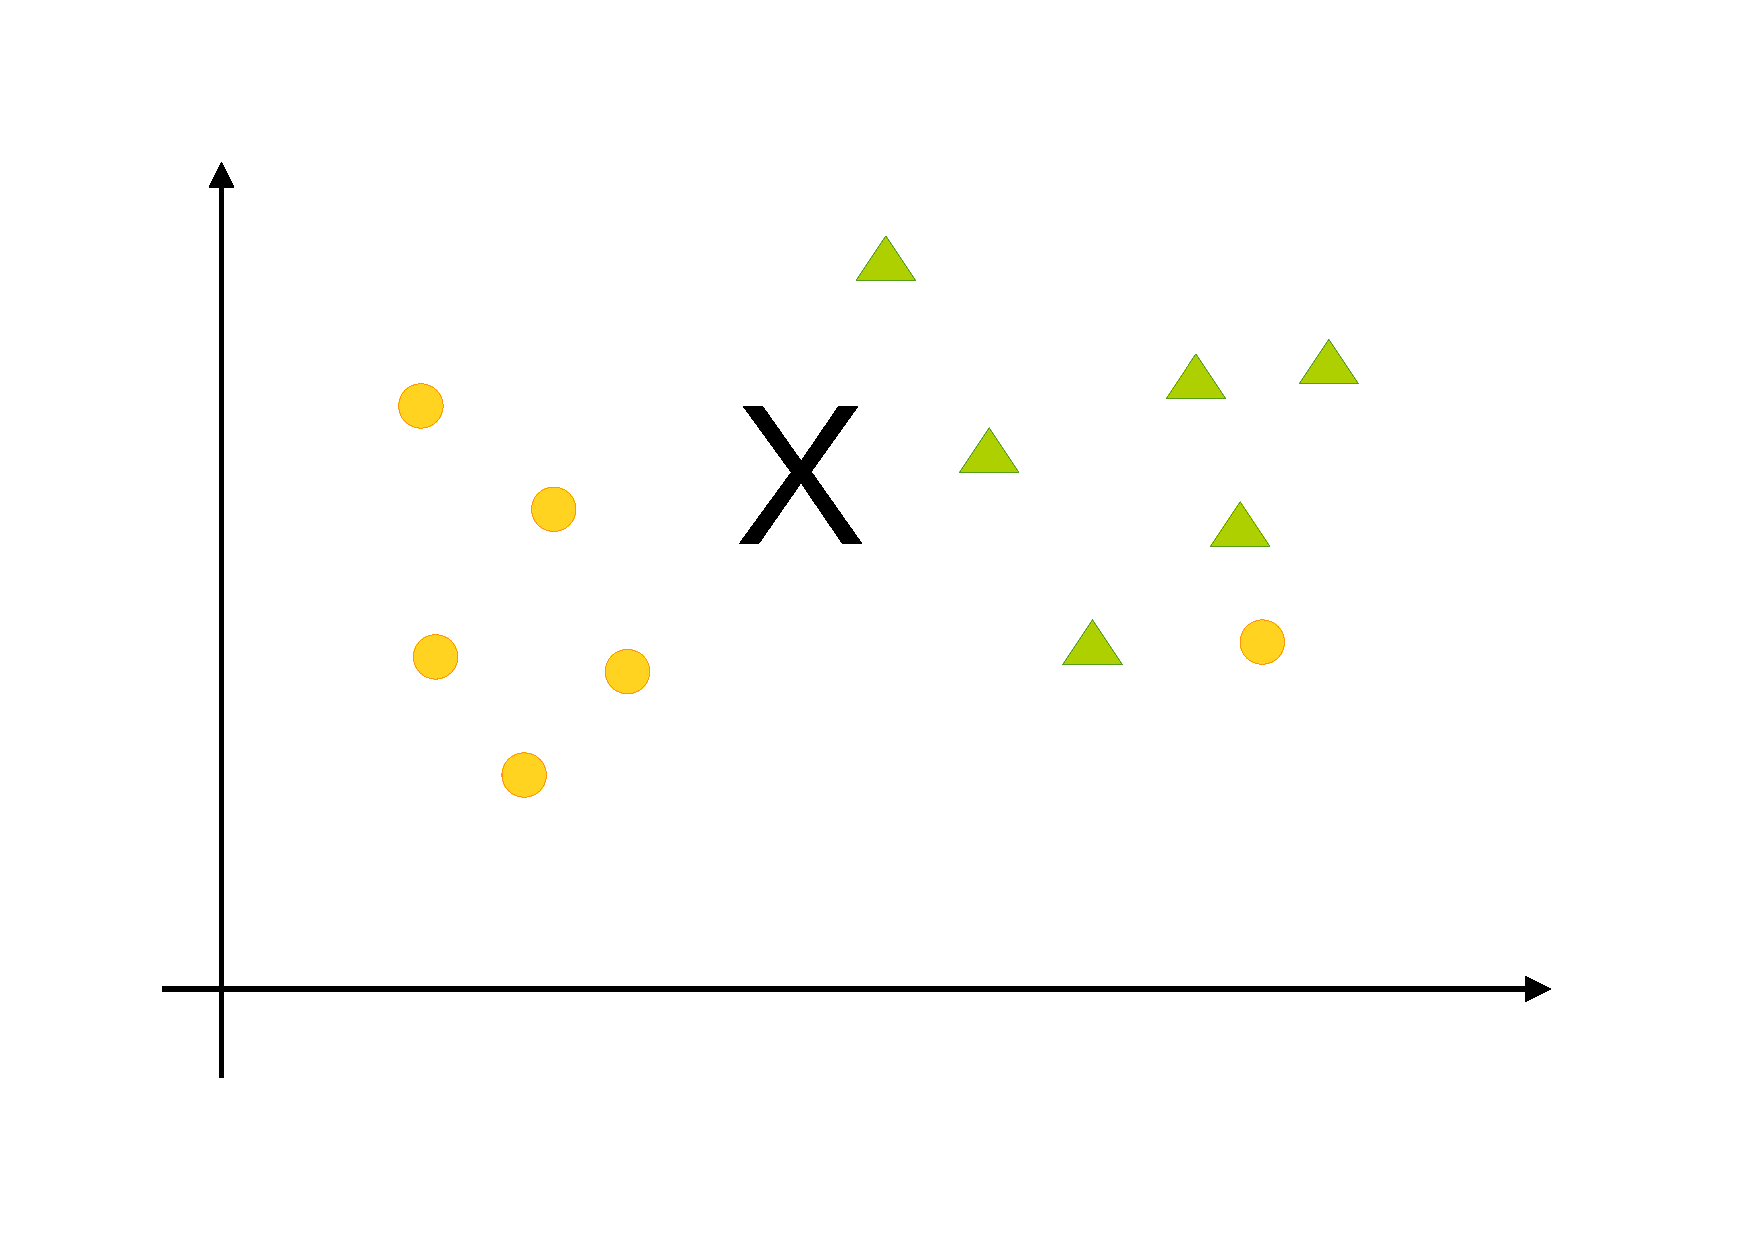
\includegraphics[width=0.7\textwidth]{images/svmm_c2.pdf}\end{center}\end{frame}
\begin{frame}\begin{center}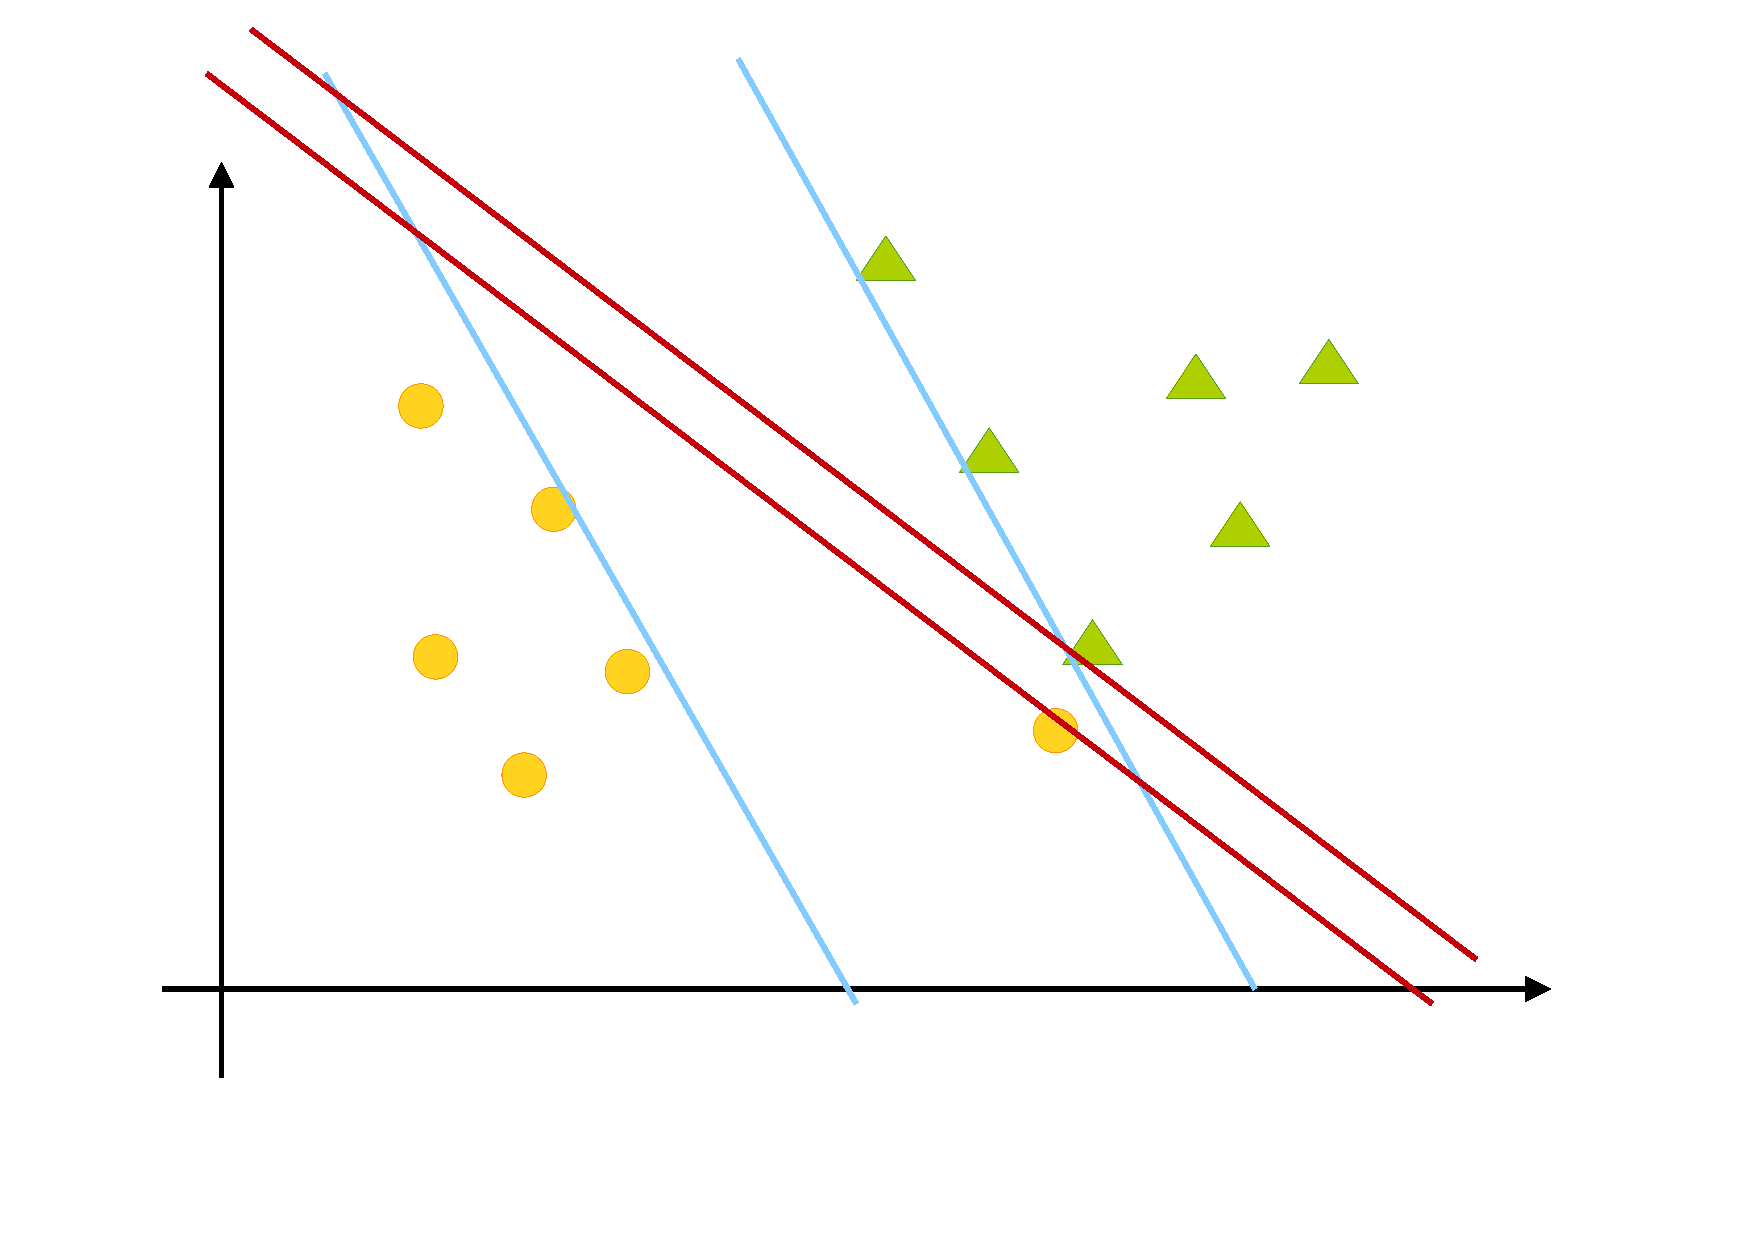
\includegraphics[width=0.7\textwidth]{images/svmm_c1.pdf}\end{center}\end{frame}


\begin{frame}{C-SVM}
	\begin{center}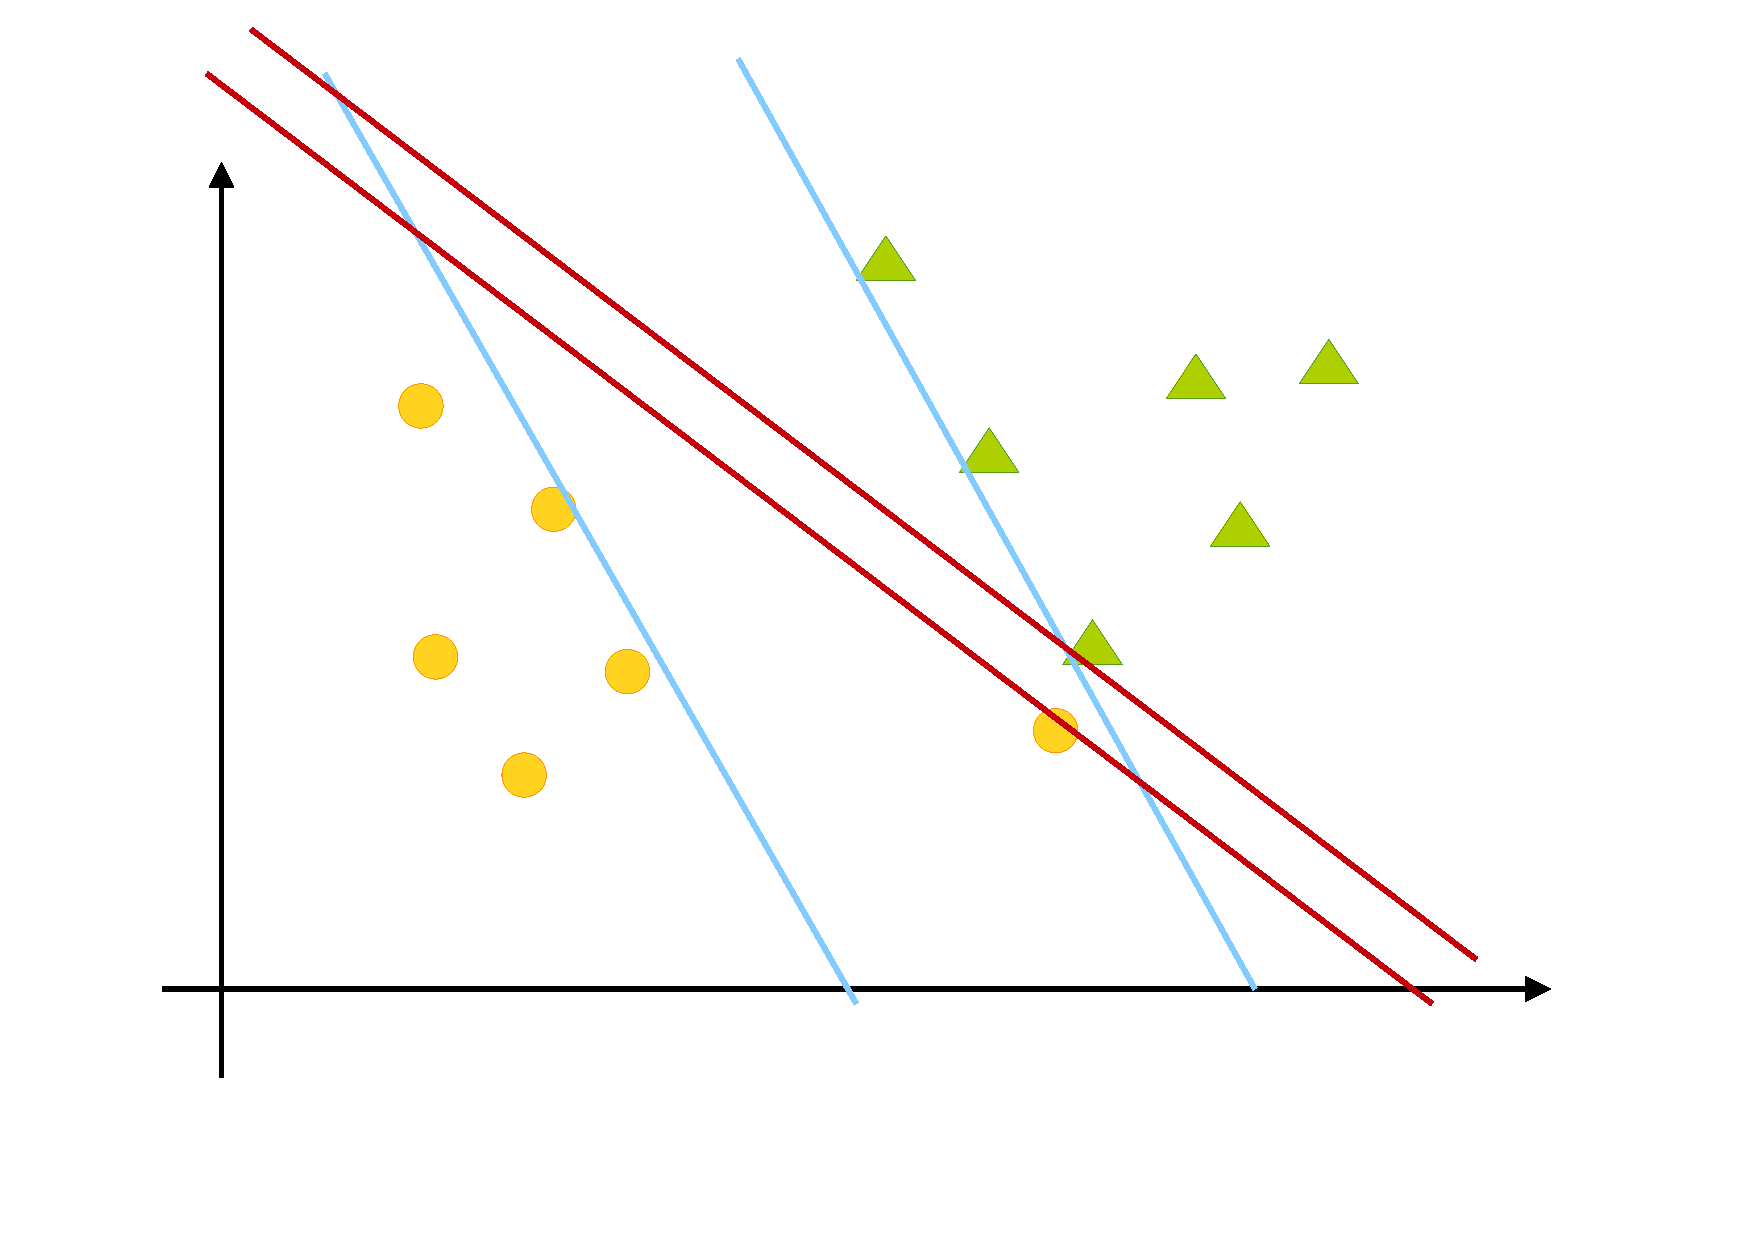
\includegraphics[width=0.25\textwidth]{images/svmm_c1.pdf}\end{center}
	\begin{itemize}
		\item Wprowadzenie do optymalizacji parametrów $\xi_i$ -- błędów klasyfikacji dla konkretnych przykładów ze zbioru treningowego
		\item Hiperparametr $C$ -- sterowanie dopasowania do danych vs wielkość marginesu
		\item C-SVM może zarówno klasyfikować zbiory niemożliwe do rozdzielenia hiperpłaszczyzną, jak i takie, w których pojedyncze przykłady zmniejszają margines
			\begin{itemize}
				\item (Wciąż liniowe rozdzielenie $\rightarrow$ metody nieliniowe)
			\end{itemize}
	\end{itemize}
\end{frame}

\section{Metody nieliniowe}

\subsection{Kernel SVM}

\begin{frame}
	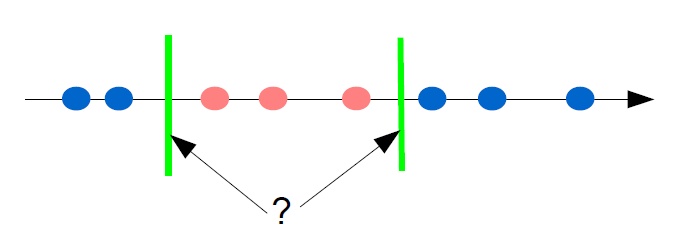
\includegraphics[width=0.3\textwidth]{images/kernel1.png}\pause \hskip 1cm $x \rightarrow x^2$ \pause \hskip 1cm 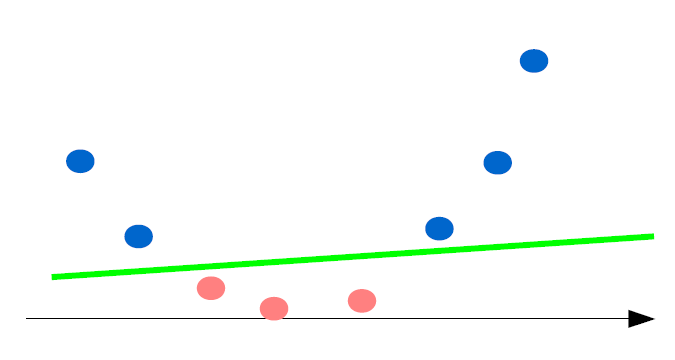
\includegraphics[width=0.3\textwidth]{images/kernel2.png}\pause \vskip 0.3 cm 
	% intuition - 1D two sides thing (no linear option), and polynomial lift allows for linear separation. So we see that moving examples to space/raum can solve
	Mapujemy dane do innej przestrzeni ($\left\{x_1, x_2, \dots \right\} \rightarrow \left\{x_1^2, x_2^2, \dots \right\}$),\pause\ mapowanie może być nieliniowe, ale w tej nowej przestrzeni istnieje możliwość liniowego rozdzielenia klas.\pause \vskip 0.3 cm 
	% lets see this, this is a mappnig x -> x. 
	W klasyfikatorze SVM, decyzja o klasyfikacji i optymalizacja wykorzystują wyłącznie iloczyn skalarny $\left\langle \cdot, \cdot \right\rangle$. \pause \vskip 0.3 cm 	
	\begin{enumerate}
		\item Możemy przetwarzać różne dane (nie tylko wektory), o ile\\\pause
dla elementów naszego zbioru danych $x_i,x_j \in \mathcal{X}$ możemy policzyć $\left\langle x_i, x_j\right\rangle$\\\pause
		\item Możemy przetwarzać przekształcenia danych $x_i \rightarrow \Phi(x_i)$, o ile\\\pause
		możemy policzyć $\left\langle \Phi(x_i), \Phi(x_j)\right\rangle$\pause \dots niekoniecznie musimy wyliczać $\Phi(x_i)$!
	\end{enumerate}	
% ..związanych z danymi, zbiór danych x (dowolny niepusty, wektory, ale moglibyśmy \begin{chciećdrzewa, albo teksty). Budujemy funkcję ktora x wciska w R lub C. jeżeli każdemu punktowi danych będziemy w stanie przypisać taką unikalną funkcję to mamy związek z danymi 
	% but all - decision, and optimization - is formulated in terms of a dot product. so find a dot product, can work 
	% compute <Phi >  - and see that it works. but is it una casa solo?
% X is arbitrary set, więc np. drzewa, grafy, obrazki, mikromacierze...
\end{frame}

\begin{frame}
	$\left\langle x_i, x_j \right\rangle = x_ix_j$\pause \vskip 0.3 cm 
	$\left\langle x_i^2, x_j^2 \right\rangle = x_i^2x_j^2 = (x_ix_j)^2 = \left\langle x_i, x_j \right\rangle^2$\pause \vskip 0.3 cm
	A może przestrzeń funkcji $f,g\in\mathcal{H}, f(x)\in\mathbb{R}, x \in\mathcal{X}$\dots $\left\langle f, g \right\rangle$?\pause \vskip 0.6 cm
% chceny jak najogólniej, bo wtedy potencjalnie największe możliwości -- ale oczywiście związanych z danymi
	Rozważmy funkcje w postaci $k: \mathcal{X} \times \mathcal{X} \rightarrow \mathbb{R}\qquad (x_i, x_j) \mapsto k(x_i, x_j)$ o cechach:
	\begin{itemize}
		\item symetryczna $k(x_i, x_j) = k(x_j, x_i)$
		\item dodatnio określona $\sum_{i,j=1}^n c_ic_j k(x_i, x_j) \geq 0  \quad \forall n \in \mathbb{N}\; \forall x_1,\dots,x_n\in\mathcal{X}\; \forall c_1, \dots, c_n \in\mathbb{R}$
	\end{itemize}\pause \vskip 0.3 cm
	Na przykład $k(x_i, x_j) = \left\langle x_i, x_j \right\rangle^2$ :) \hskip 1cm (a ogólnie $k(x_j, x_i) = \left(\left\langle x_i, x_j \right\rangle + c\right)^d, c\geq 0, d\in\mathbb{N}$)\pause \vskip 0.3 cm 
	Dla $x_1 = 42$, możemy zbudować funkcję $k_1(x) = \left\langle x, 42 \right\rangle^2 = 1764x^2$\pause
	\begin{itemize}
		\item Dla punktów danych $x_i\in\mathcal{X}$ mamy funkcje $k(x_i, x)\in\mathbb{R}$ -- przestrzeń funkcji
		\item  $\left\langle k(x_i, x), k(x_j, x) \right\rangle$?
	\end{itemize}
\end{frame}

\begin{frame}
$\left\langle k(x_i, x), k(x_j, x) \right\rangle$?\pause\vskip 0.3 cm
Jeżeli funkcja w postaci $k: \mathcal{X} \times \mathcal{X} \rightarrow \mathbb{R}\quad (x_i, x_j) \mapsto k(x_i, x_j)$ jest symetryczna i dodatnio określona, to\pause\ (twierdzenie Moore'a–Aronszajna) istnieje przestrzeń Hilberta funkcji określonych na $\mathcal{X}$ w której $k$ jest reprodukującym jądrem (reproducing kernel).\vskip 0.3 cm
\begin{itemize}
	\item Przestrzeń Hilberta -- przestrzeń liniowa (dodawanie, mnożenie przez skalar) + zdefiniowany iloczyn skalarny który indukuje metrykę (możemy wyznaczyć odległość między elementami zbioru)
	\item Przestrzeń Hilberta z reprodukującym jądrem (RKHS) -- dla każdego $x_i\in\mathcal{X}$ istnieje funkcja $k_{x_i}\in\mathcal{H}$ taka że dla każdej funkcji z tej przestrzeni $f\in\mathcal{H}$ zachodzi $\left\langle f, k_{x_i} \right\rangle = f(x_i)$
\end{itemize}\pause \vskip 0.3 cm
$\left\langle k(x_i, x), k(x_j, x) \right\rangle = k(x_i, x_j)$
%Funkcje $k_i(x) = k(x_i, x)\in\mathbb{R}$
%\begin{itemize}
%	\item Dla każdego $x_i\in\mathcal{X}$ istnieje funkcja $k(x_i, x)$\pause
%	\item Dla każdej funkcji w tej przestrzeni $f\in\mathcal{H}$ -- $k_j(x) = k(x_j, x)$ dla każdego $x_j$\pause
%	\item Zachodzi $\left\langle f, k_{x_i} \right\rangle = f(x_i) = k_j(x_i) = k(x_j, x_i)$
%\end{itemize}
\end{frame}

\begin{frame}
\begin{center}
	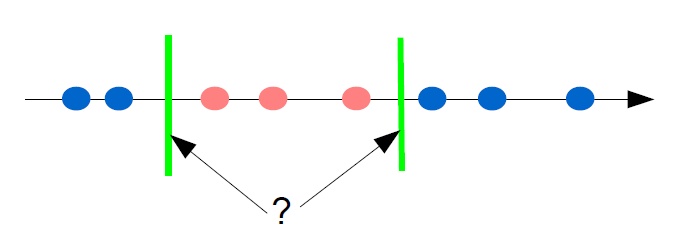
\includegraphics[width=0.13\textwidth]{images/kernel1.png}\hskip 0.5cm $\rightarrow$\hskip 0.5cm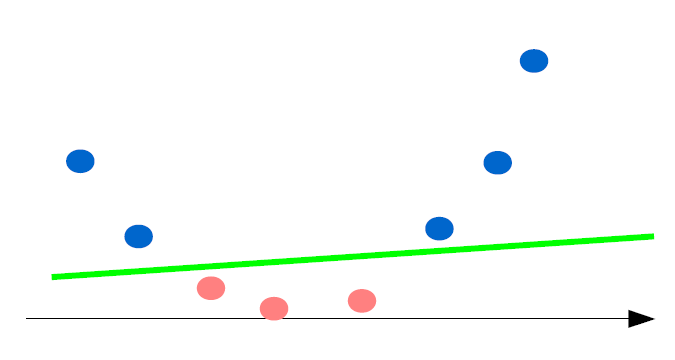
\includegraphics[width=0.13\textwidth]{images/kernel2.png}\vskip 0.3 cm 
\end{center}
Podsumowanie:
\begin{enumerate}
	\item Mamy zbiór danych $\mathcal{X}$, o złożonej strukturze (nieliniowa granica decyzyjna)
	\item Mamy narzędzie liniowej klasyfikacji, oparte o iloczyn skalarny
	\item Szukamy nieliniowego przekształcenia danych do innej przestrzeni, gdzie możemy liniowo rozdzielić klasy
	\item Jeżeli znajdziemy dobrą funkcję $k$, to dzięki własnościom RKHS możemy odwzorować dane w innej przestrzeni $\mathcal{H}$, opartej o $k$, w której wyliczymy iloczyn skalarny jako $k(x_i, x_j)$
	\item Ponieważ odwzorowanie jest nieliniowe, liniowe rozdzielenie w $\mathcal{H}$ przekłada się na nieliniową granicę decyzyjną w $\mathcal{X}$
\end{enumerate}
\end{frame}

\begin{frame}
\begin{center}
	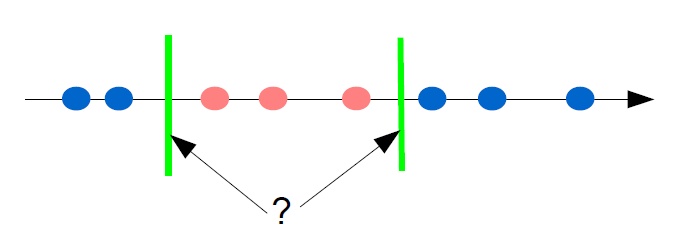
\includegraphics[width=0.13\textwidth]{images/kernel1.png}\hskip 0.5cm $\rightarrow$\hskip 0.5cm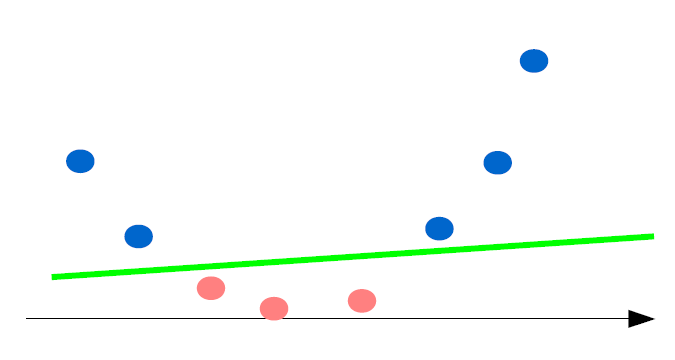
\includegraphics[width=0.13\textwidth]{images/kernel2.png}\vskip 0.3 cm 
\end{center}
SVM $\mathbf{y} = \mathrm{sgn}\left(\sum_i \alpha_i\left\langle \mathbf{x}_i, \mathbf{x} \right\rangle + b\right) \quad \rightarrow \quad \text{kernel-SVM}\; \mathbf{y} = \mathrm{sgn}\left(\sum_i \alpha_i k(\mathbf{x}_i, \mathbf{x}) + b\right)$\vskip 0.3 cm 
Popularne funkcje $k$:
\begin{itemize}
	\item RBF $k( \mathbf{x}_i,  \mathbf{x}_j) = e^{-\gamma \| \mathbf{x}_i -  \mathbf{x}_j \|^2} $ \vskip 0.7 cm
	\item Wielomianowa $k( \mathbf{x}_i,  \mathbf{x}_j) = \left(\left\langle  \mathbf{x}_i, \mathbf{x}_j \right\rangle + c\right)^d, c\geq 0, d\in\mathbb{N}$	
	\item Sigmoid $k( \mathbf{x}_i,  \mathbf{x}_j) = \dots $
\end{itemize}\pause\vskip 0.3 cm
Najczęściej wystarczy jedna dobra funkcja -- RBF
\end{frame}

\begin{frame}
\begin{center}
	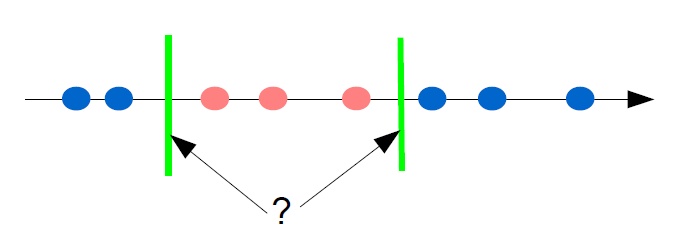
\includegraphics[width=0.13\textwidth]{images/kernel1.png}\hskip 0.5cm $\rightarrow$\hskip 0.5cm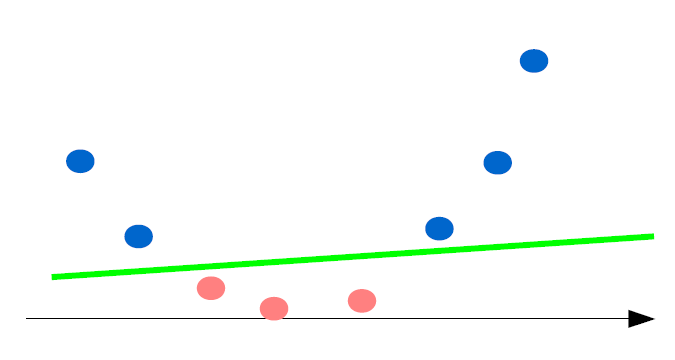
\includegraphics[width=0.13\textwidth]{images/kernel2.png}\vskip 0.3 cm 
\end{center}
	\emph{	 The idea of SVMs: map the training data into a higher-dimensional feature space via $\Phi$, and construct a separating hyperplane with maximum margin there. This yields a nonlinear decision boundary in input space. By the use of a kernel function, it is possible to compute the separating hyperplane without explicitly carrying out the map into the feature space}
	\begin{flushright}
		Learning with Kernels, str. 29
	\end{flushright}
\end{frame}

\begin{frame}
	Przykłady funkcji jądrowych: liniowa, wielomianowa, RBF
	\begin{center}
		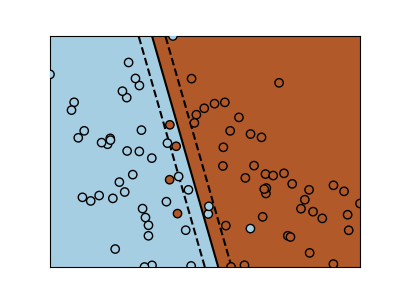
\includegraphics[width=0.3\textwidth]{images/linear.png}
		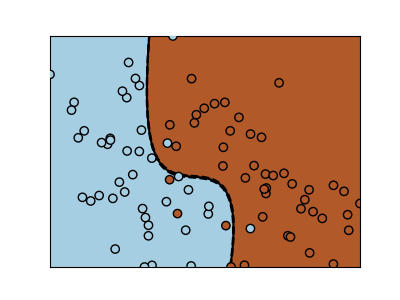
\includegraphics[width=0.3\textwidth]{images/polynomial.png}
		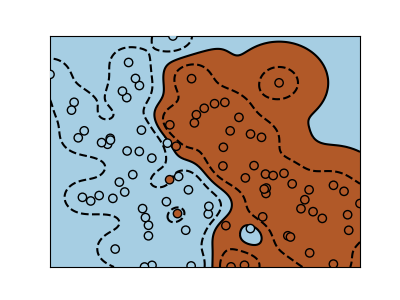
\includegraphics[width=0.3\textwidth]{images/rbf.png}
	\end{center}
\end{frame}

\begin{frame}
	Przykłady funkcji jądrowej RBF dla różnych wartości parametru $\gamma$,\\kolejno wartości $\gamma$: dopasowana do zbioru danych, niska, wysoka
	\begin{center}
		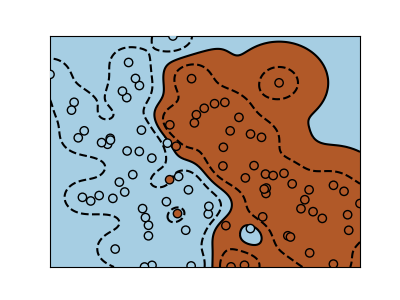
\includegraphics[width=0.3\textwidth]{images/rbf3opt.png}
		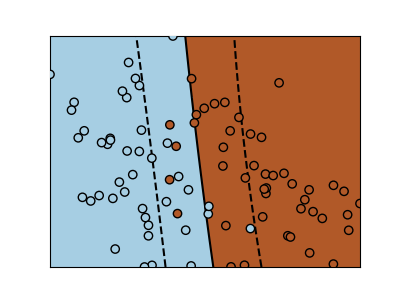
\includegraphics[width=0.3\textwidth]{images/rbf2low.png}
		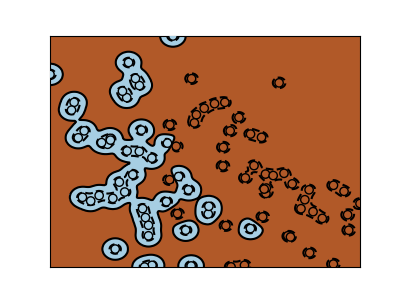
\includegraphics[width=0.3\textwidth]{images/rbf1high.png}
	\end{center}
\end{frame}

\begin{frame}
	Przykłady funkcji jądrowej RBF dla dopasowanej do danych wartości $\gamma$,\\kolejno wartości $C$: niska, dopasowana, wysoka
	\begin{center}
		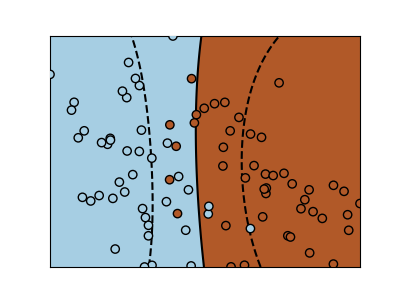
\includegraphics[width=0.3\textwidth]{images/rbfclow.png}
		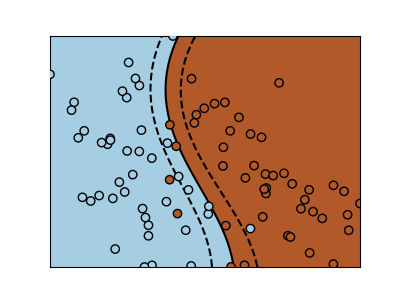
\includegraphics[width=0.3\textwidth]{images/rbfcmid.png}
		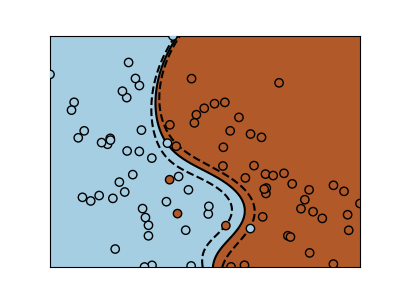
\includegraphics[width=0.3\textwidth]{images/rbfchigh.png}
	\end{center}
\end{frame}

% ?? examples gaussian kernel from the neuron stuff -- postmortem że tu simple machinery that deals with them, but if too much data, networks scale better

\begin{frame}
	Kernel SVM:
	\begin{itemize}
		\item Skuteczny w praktyce klasyfikator
		\item Bardzo dobrze opracowany teoretycznie
		\item Dwa -- tylko dwa -- hiperparametry, o łatwej interpretacji
		\item ,,Kernel trick'' -- możliwość uogólnienia algorytmów dających się sformułować w oparciu o iloczyn skalarny (np. PCA $\rightarrow$ kernel PCA)
	\end{itemize}
\vskip 1cm
	\begin{center}
		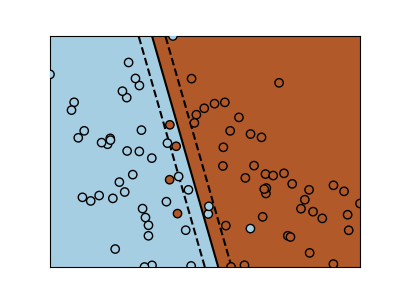
\includegraphics[width=0.1\textwidth]{images/linear.png}
		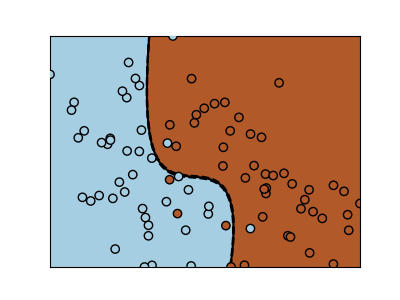
\includegraphics[width=0.1\textwidth]{images/polynomial.png}
		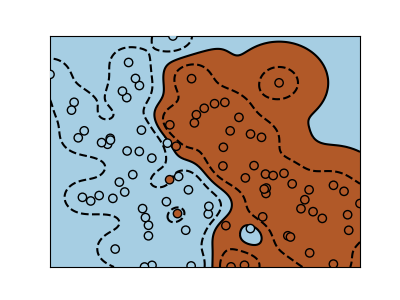
\includegraphics[width=0.1\textwidth]{images/rbf.png}
		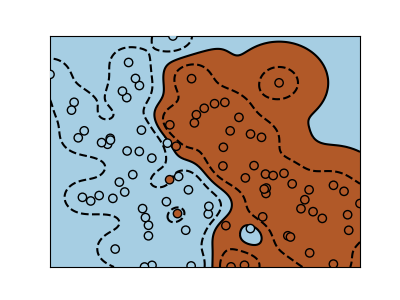
\includegraphics[width=0.1\textwidth]{images/rbf3opt.png}
		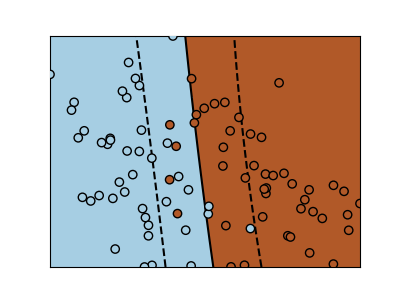
\includegraphics[width=0.1\textwidth]{images/rbf2low.png}
		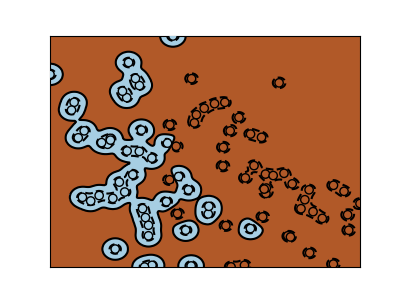
\includegraphics[width=0.1\textwidth]{images/rbf1high.png}
		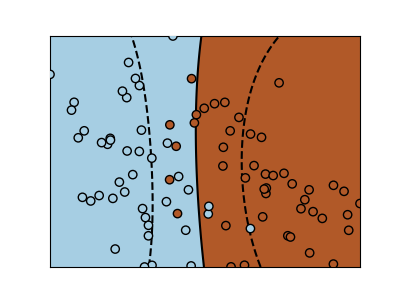
\includegraphics[width=0.1\textwidth]{images/rbfclow.png}
		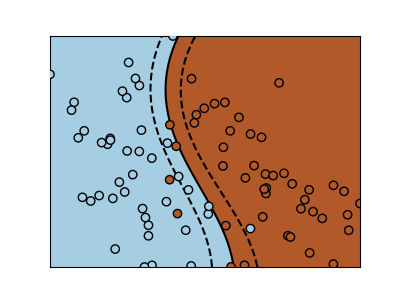
\includegraphics[width=0.1\textwidth]{images/rbfcmid.png}
		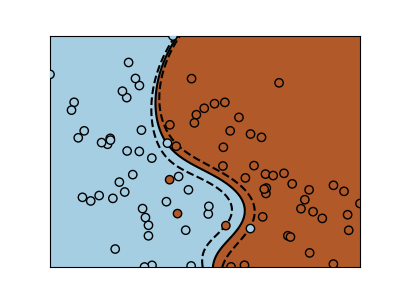
\includegraphics[width=0.1\textwidth]{images/rbfchigh.png}
	\end{center}
\end{frame}



\section{Pomiar wydajności klasyfikatorów}

\begin{frame}
	\begin{itemize}
		\item Skąd wiemy, jak dobry jest klasyfikator?
		\item Kiedy jeden klasyfikator jest lepszy od drugiego?
		\item Jak diagnozować problem z wydajnością/skutecznością?
	\end{itemize}
\end{frame}

\subsection{Miary wydajności}

\begin{frame}
	\begin{itemize}
		\item Skuteczność (accuracy) $\frac{T}{T + F}$\only<6->{\hskip 0.3 cm$\frac{TP + TN}{TP+FN+FP+TN}$ }\pause
			\begin{itemize}
				\item Intuicyjna, naturalna\pause
				\item Wrażliwa na różną liczebność klas\pause
				\item Wrażliwa na rodzaj błędów\pause
			\end{itemize}
		\item Macierz błędów (confusion matrix)
% nuclear power plant, medical patient state classification
		\tiny 
    \renewcommand{\arraystretch}{1.5} % Adjust row height
\setlength{\tabcolsep}{10pt}     % Adjust column width
\begin{tabular}{|c|c|c|}
	\hline
	& \textbf{Predicted Positive} & \textbf{Predicted Negative} \\
	\hline
	\textbf{Actual Positive} & TP (True Positive) & FN (False Negative) \\
	\hline
	\textbf{Actual Negative} & FP (False Positive) & TN (True Negative) \\
	\hline
\end{tabular}
\normalsize\pause
	\item Precison $\frac{TP}{TP + FP}$  oraz recall $\frac{TP}{TP + FN}$ \pause
% Precision (also called positive predictive value) is the fraction of relevant instances among the retrieved instances.  Recall (also known as sensitivity) is the fraction of relevant instances that were retrieved. Both precision and recall are therefore based on relevance. 
	\item Sensitivity (czułość) $\frac{TP}{TP + FN}$ oraz specificity (swoistość) $\frac{TN}{TN + FP}$\pause
%  then sensitivity is a measure of how well a test can identify true positives and specificity is a measure of how well a test can identify true negatives: Sensitivity (true positive rate) is the probability of a positive test result, conditioned on the individual truly being positive . Specificity (true negative rate) is the probability of a negative test result, conditioned on the individual truly being negative.
	\item True positive ratio $\frac{TP}{TP + FN}$  oraz false positive ratio $\frac{FP}{FP + TN}$\pause 
	\item F1 score $\frac{2}{p^{-1} + r^{-1}}=2\frac{p \times r}{p + r} = \frac{2TP}{2TP + FP + FN}$
% harmonic mean of p and r
%  Without loss of generality consider a binary classification task. Imagine having a data which of 100 samples with 90 negative sample and 10 positive sample. Suppose you have a classifier that predicts all negative. You will have an accuracy of 90%, but let's consider the f1 score, you will actually get 0 because your recall (which is a component of f1 score) is 0. 

	\end{itemize}
\end{frame}

\begin{frame}
	Jeden klasyfikator, wydajność -- niezależnie od hiperparametrów?\pause\vskip 0.3 cm
	Prosty klasyfikator (średnie klas), progowanie szacowanego prawopodobieństwa $T=0.1$
	\begin{center}	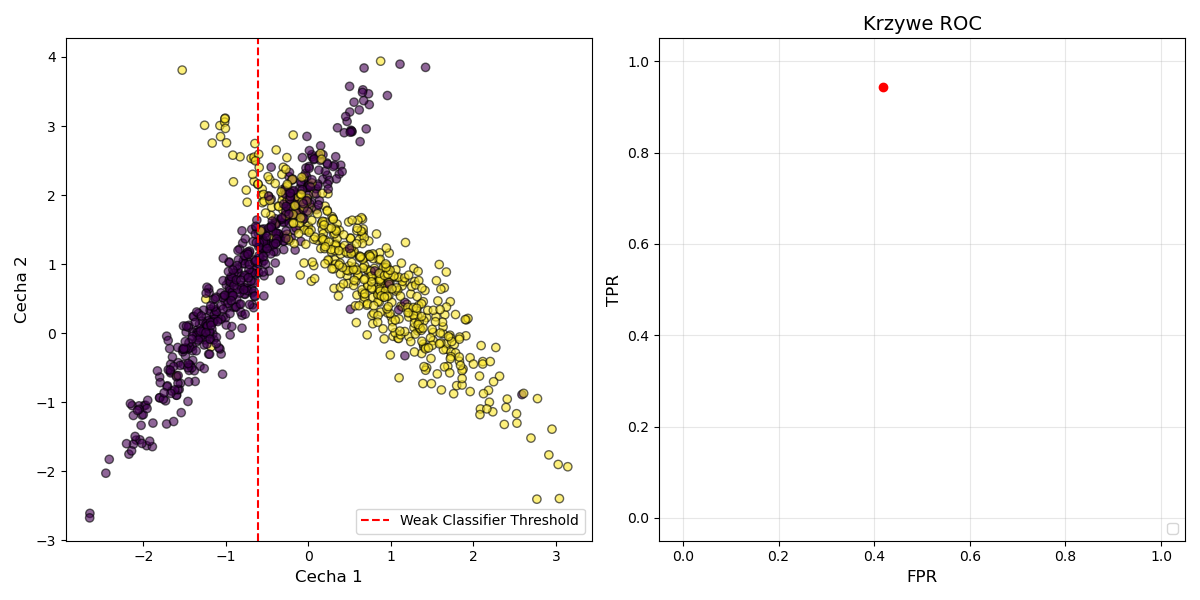
\includegraphics[width=0.8\textwidth]{images/roc1.png} \end{center}
\end{frame}
\begin{frame}
	Prosty klasyfikator (średnie klas), progowanie szacowanego prawopodobieństwa $T=0.5$
	\begin{center}	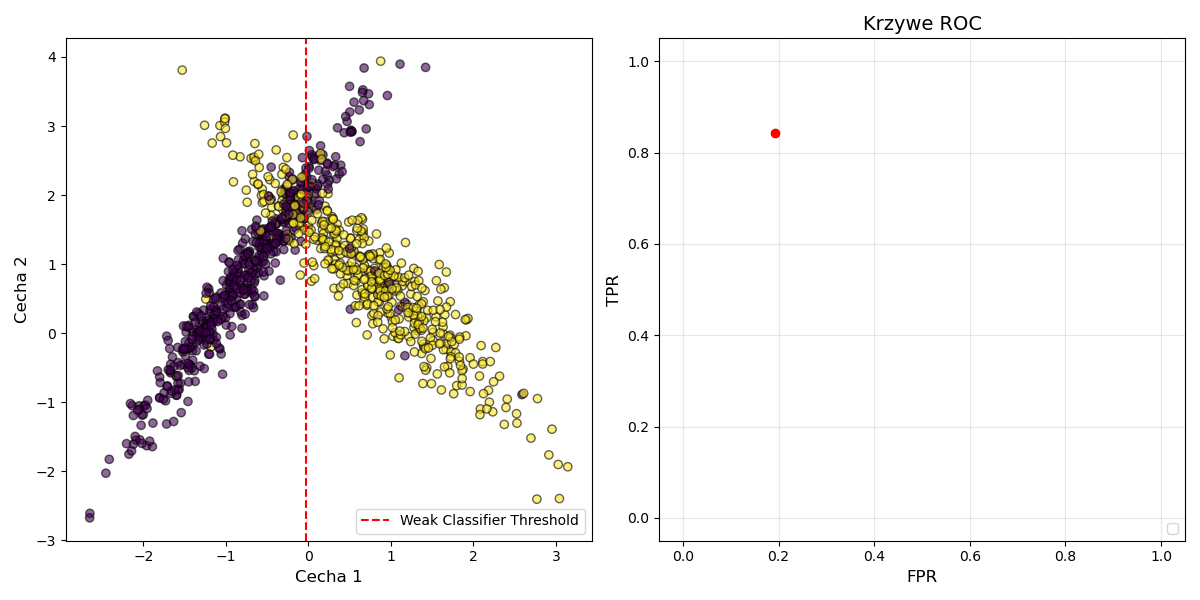
\includegraphics[width=0.8\textwidth]{images/roc2.png} \end{center}
\end{frame}
\begin{frame}
	Prosty klasyfikator (średnie klas), progowanie szacowanego prawopodobieństwa $T=0.9$
	\begin{center}	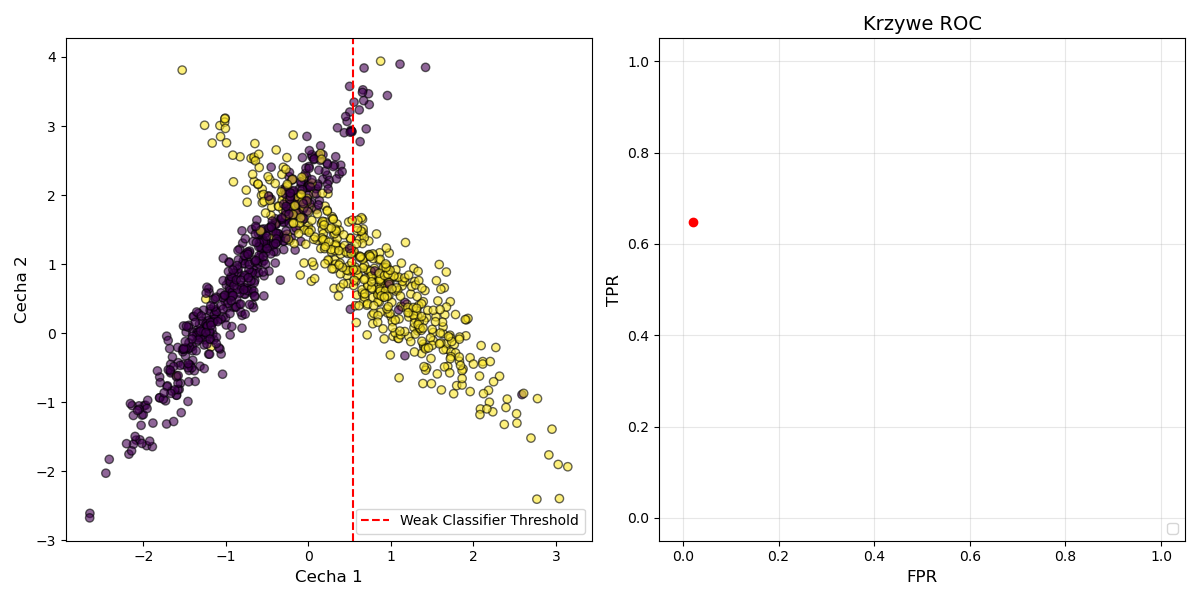
\includegraphics[width=0.8\textwidth]{images/roc3.png} \end{center}
\end{frame}
\begin{frame}
	Prosty klasyfikator (średnie klas), progowanie szacowanego prawopodobieństwa -- krzywa charakterystyki operatora (receiver operator characteristic, ROC)
	\begin{center}	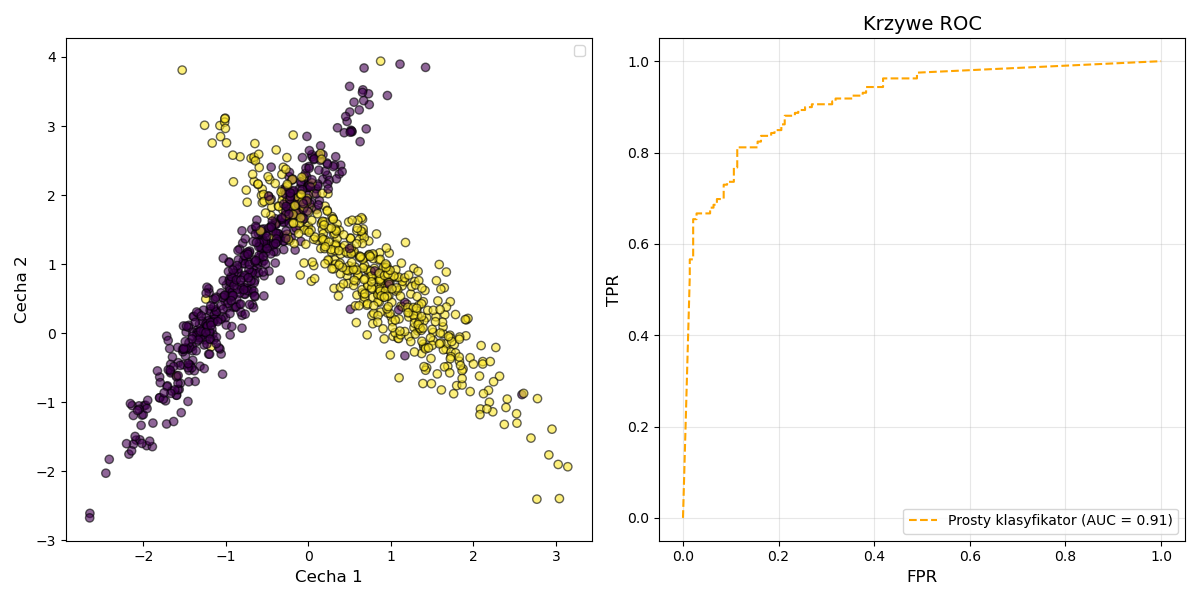
\includegraphics[width=0.8\textwidth]{images/roc4.png} \end{center}
\end{frame}
\begin{frame}
	Prosty klasyfikator vs SVM -- krzywe ROC
	\begin{center}	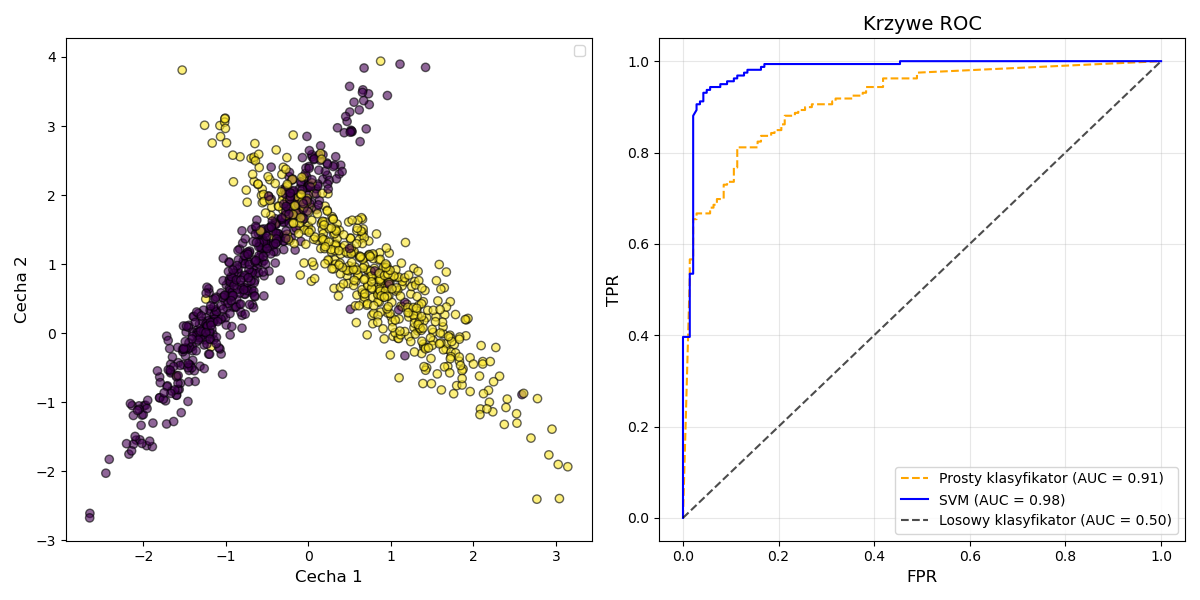
\includegraphics[width=0.8\textwidth]{images/roc5.png} \end{center}
\end{frame}

\begin{frame}
	Dwa klasyfikatory, wydajność, porównanie?\pause\vskip 0.3 cm
	Np. 88\% vs 89\%\pause\ - a co jeżeli to przypadek, i na innej części zbioru danych będzie 89\% vs 88\%?\pause\vskip 0.3 cm
	(alternatywnie -- który zestaw hiperparametrów wybrać?)\pause\vskip 0.3 cm
	\begin{enumerate}
		\item Testy statystyczne ($\rightarrow$ wykłady dr hab. Hanna Wojewódka-Ściążko)\pause
		\item Pary wyników (dla konkretnego punktu danych wyniki obu klasyfikatorów) -- różnice\pause
		\item Czy mają rozkład normalny (test Shapiro-Wilk)?\pause
		\item Jeżeli tak (r.n.) -- t-test dla par
			\begin{itemize}
				\item Hipoteza zerowa tego testu mówi o równych średnich, a alternatywna o
				różnych, zatem odrzucenie hipotezy zerowej świadczy o tym, że wyniki jednej
				z metod są istotnie statystycznie różne od drugiej
				\item Jednostronnie lub dwustronnie
			\end{itemize}
		\item Jeżeli nie (r.n.) -- Wilcoxon signed-rank test\pause
		\item Testy pozwalają określić szansę (przez p-wartość) odpowiedniości lub przewagi klasyfikatorów
	\end{enumerate}
	% comparing classifiers - statistical tests 
\end{frame}

\subsection{Walidacja krzyżowa}

\begin{frame}
	Klasyfikator, skuteczność 89\% \dots oczekiwania? \pause Spodziewany wynik ,,w działaniu'', najlepsze możliwe oszacowanie, prawdziwa skuteczność klasyfikacji, powtarzalność, uogólnianie\dots
	\begin{itemize}
		\item Zbiór danych -- reprezentatywny dla problemu\pause
		\item Wydzielenie zbioru testowego:
			\begin{itemize}
				\item Brak -- oszacowanie obciążone (skuteczność zawyżona)
				\item 50\% trening, 50\% test -- oszacowanie obciążone (skuteczność zaniżona)
				\item Wydzielenie pojedynczego przykładu (leave one out) + powtarzanie -- duża wariancja, złożone obliczeniowo
					\begin{itemize}
						\item Ale -- leave one patient out!
					\end{itemize}
				\item Wydzielenie części (np. 5, 10, 20\%) i powtórzenie -- walidacja krzyżowa, optymalne\pause
				\item Wydzielenie zbioru testowego -- niezależna weryfikacja wydajności
			\end{itemize}\pause
		\item Wydzielenie zbioru walidacyjnego\pause
			\begin{itemize}
				\item Skąd wiemy jakie hiperparametry ustawić?\pause
				\item Wewnętrzna pętla walidacji żeby ustalić wartości hiperparametrów
				\item Dwa poziomy walidacji (zewnętrzna -- zbiór testowy, wewnętrzna -- zbiór walidacyjny) -- niezależna weryfikacja wydajności uwzględniająca niepewność doboru hiperparametrów
					\begin{itemize}
						\item Testowanie metody vs testowanie metody z hiperparametrami dobranymi przez eksperta
					\end{itemize}
			\end{itemize}
	\end{itemize}
	
	
\end{frame}

\subsection{Analiza jakościowa (danych i wyników)}

\begin{frame}
	Klasyfikator, 89\% \pause zweryfikowana walidacją krzyżową, dobór parametrów OK -- co dalej?\pause\\
	Analiza ilościowa -- miary skuteczności\\
	Analiza jakościowa -- przegląd wyników pod kątem outlierów, regularności, wzorców itp.\pause
	\begin{itemize}
		\item Szukaj outlierów i anomalii\only<4>{
			\begin{center}	
			
\includegraphics[width=0.4\textwidth]{images/sphx_glr_plot_anomaly_comparison_001.png} 
			\end{center}
			\begin{flushright}
			{\tiny dokumentacja sklearn, BSD}\hskip 2 cm\mbox{ }
			\end{flushright}
			}\pause
		\item Zobacz jak się grupują przykłady (np. w obrębie klas)\only<5>{
			\begin{center}	
				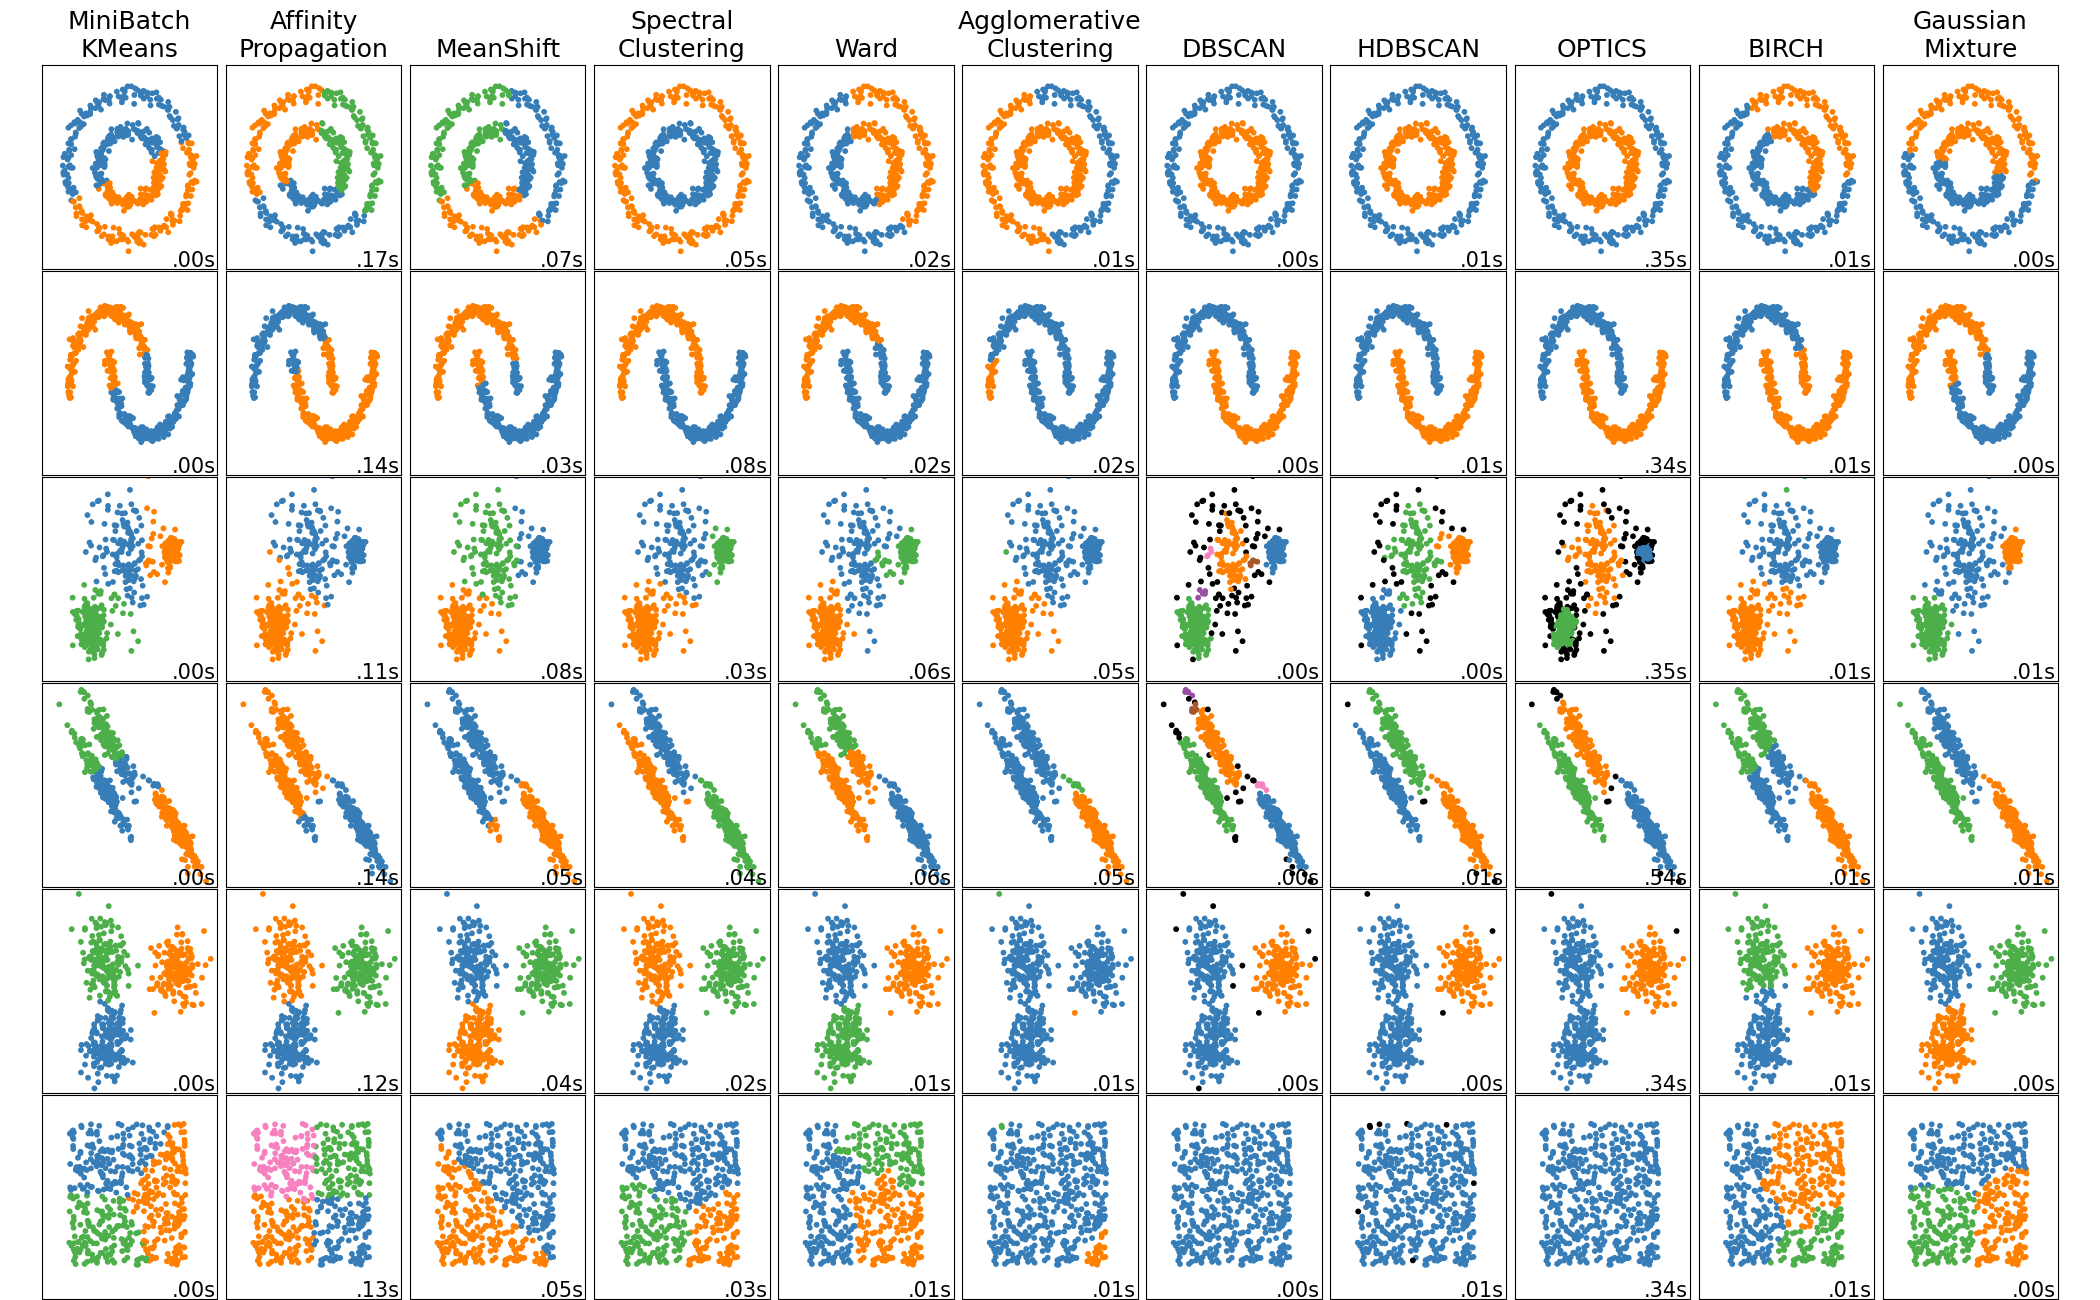
\includegraphics[width=0.5\textwidth]{images/sphx_glr_plot_cluster_comparison_001.png} 
			\end{center}
			\begin{flushright}
				{\tiny dokumentacja sklearn, BSD}\hskip 2 cm\mbox{ }
			\end{flushright}
		}\pause
		\item Stosuj redukcję wymiarowości (dla wizualizacji)\only<6>{
			\begin{itemize}
				\item PCA
				\item tSNE
				\item kernel PCA, ICA, NMF, \dots
			\end{itemize}
			}\pause	
		\item Próbuj prostych metod\only<7>{
			\begin{itemize}
				\item SVM, RF, MLP
				\item kNN, 1-NN
				\item Regresja liniowa
			\end{itemize}
		}\pause	
		\item Wizualizuj co tylko się da\only<8>{
		\begin{itemize}
				\item Histogramy/wykresy pudełkowe błędów
				\item Przykłady dobrze i źle sklasyfikowane
				\item Test wizualnej identyfikacji wzorców
				\item Zależność od zewnętrznych parametrów 
		\end{itemize}}\pause
		\vskip 1cm
		\item Powodzenia :)
	\end{itemize}
\end{frame}


% analiza ilościowa -- miary 

% na koniec podsumka tego co planowałem zrobić na dodatkowym wykładzie - toolbox analizy danych - będzie na zajęciach ale cotam
% grupowańsko i redukcja wymiarowości 

% kmeans, hierarchical, dbscan, MoG
% PCA, tsne, ica?nmf? kPCA
% outlier/anomaly detector 
% basic classifier tests, esp SVM, RF, MLP
% ..and plot everything. don't look too hard, when you see it, you see it. 
%  Przykłady:  (nie licząc znalezionych otulierów itp) ? just two classes problematic   ? wysypy o różnej strukturze, więc zależy co do zbioru testowego trafi -- hsi classification 
%   - hsi camera spatial error 
%   - not representing at all - spectral  reconstruction
%   - failed networks due to bad initalization 
%   - mislabels - randomowe zdjęcia ulicy złapało twarz na plakacie 

\end{document}

